\chapter{数据可视化}

本书第一部分的目标是让你尽快掌握数据探索的基本工具。数据分析的流程大致如下:

\begin{figure}[htbp]
  \centering
  
\includegraphics[width=\textwidth]{assets/数据分析流程.png}
  \caption{数据分析的基本流程}\label{fig:datawf}
\end{figure}

在这一部分你会学习到一些有用的工具:

\begin{enumerate}
\item  绘图是学习 Stata 的一个很好的开始,这是因为绘图能够最快地给使用者成就感。在数据可视化部分你讲学习到一些基本的绘图方法和一些有用的数据处理技巧。
\item  仅仅学习绘图是不够的,你还需要学习一些数据变换的方法,这样你才能根据自己的需要展示数据。
\item  最后,当你掌握了一些数据变换和绘图的方法之后,你就可以对一些实际案例进行分析了。
\end{enumerate}

接下来的三章将分别介绍数据可视化、数据整理和数据探索性分析。

\section{准备工作}

作者认为 Stata 的默认绘图主题不怎么好看,所以建议不要使用,推荐使用 plotplain 主题,安装方法如下:

\begin{lstlisting}
* 安装主题包
net install gr0070, from("http://www.stata-journal.com/software/sj17-3") replace
* 设置 plotplain 会默认绘图主题
set scheme plotplain, permanently
\end{lstlisting}

关于 Stata 绘图主题的选择,可以参考 \href{https://blog.stata.com/2018/10/02/scheming-your-way-to-your-favorite-graph-style/}{Scheming your way to your favorite graph style} 和 \href{https://www.czxa.top/posts/24695/}{Stata的绘图主题}。

\section{第一步}

\begin{problem}
  让我们用图表回答这么一个问题:大排量的汽车是否比小排量的汽车使用更多的燃料?你可能已经有了答案,但是图表可以让你的答案更有说服力,发动机的功率和燃油效率之间的关系是怎样的,是正相关么?是线性的么?
\end{problem}

\subsection{读入 mpg 数据}

这个数据集来源于 R 的 ggplot2 包,mpg 数据集包含了美国环保局收集的 38 种型号的汽车的数据:

\begin{lstlisting}
cd ~/Documents/我的项目/stata4ds/
sysuse mpg, clear
\end{lstlisting}

表 \ref{tab:mpg} 展示了 mpg 数据集的一部分。

\begin{table}[htbp]
\caption{\label{tab:mpg}mpg 数据概览}
\centering
\begin{tabular}{ccccccccccc}
\toprule
manufacturer & model & displ & year & cyl & trans & drv & cty & hwy & fl & class\\
\midrule
audi & a4 & 1.8 & 1999 & 4 & auto(l5) & f & 18 & 29 & p & compact\\
audi & a4 & 1.8 & 1999 & 4 & manual(m5) & f & 21 & 29 & p & compact\\
audi & a4 & 2.0 & 2008 & 4 & manual(m6) & f & 20 & 31 & p & compact\\
audi & a4 & 2.0 & 2008 & 4 & auto(av) & f & 21 & 30 & p & compact\\
audi & a4 & 2.8 & 1999 & 6 & auto(l5) & f & 16 & 26 & p & compact\\
\addlinespace
audi & a4 & 2.8 & 1999 & 6 & manual(m5) & f & 18 & 26 & p & compact\\
audi & a4 & 3.1 & 2008 & 6 & auto(av) & f & 18 & 27 & p & compact\\
audi & a4 quattro & 1.8 & 1999 & 4 & manual(m5) & 4 & 18 & 26 & p & compact\\
audi & a4 quattro & 1.8 & 1999 & 4 & auto(l5) & 4 & 16 & 25 & p & compact\\
audi & a4 quattro & 2.0 & 2008 & 4 & manual(m6) & 4 & 20 & 28 & p & compact\\
\bottomrule
\end{tabular}
\end{table}

其中:
1. dipl 变量为发动机的排量,单位为升;
2. hwy 变量是汽车在高速公路上的燃油效率,以每加仑汽油前进英里数(mpg)计算。当行驶相同距离时,具有低燃油效率的汽车消耗更多的燃料。

\subsection{创建散点图}

\texttt{scatter} 命令的基本用法是 \texttt{scatter\ y\ x},如图 \ref{fig:hwydispl}:

\begin{lstlisting}
twoway scatter hwy displ
\end{lstlisting}

\begin{figure}[htbp]
  \centering
  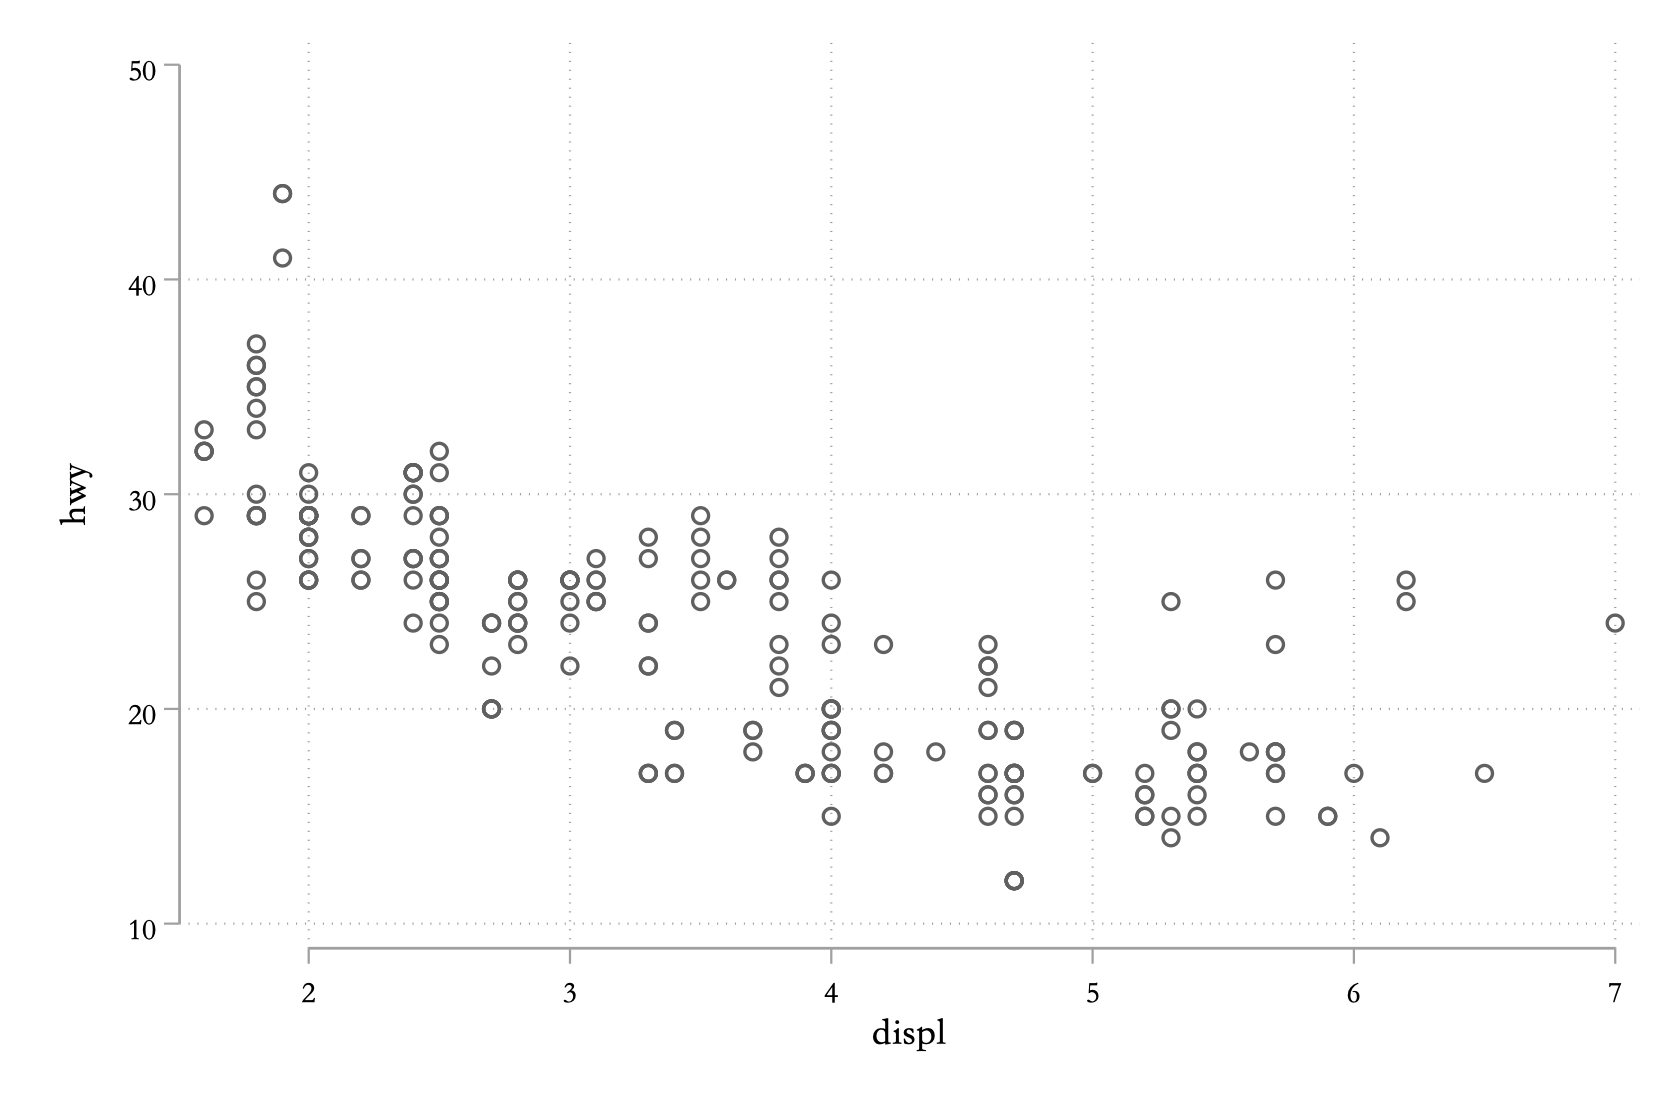
\includegraphics[width=\textwidth]{assets/hwydispl.png}
  \caption{汽车排量与燃油效率}
  \label{fig:hwydispl}
\end{figure}

图 \ref{fig:hwydispl} 显示了发动机排量和燃油效率之间的负相关关系,换句话来说,汽车的排量越高,燃油效率越低。

\subsection{练习}

\begin{exercise}
  运行 \lstinline{sc hwy displ},你看到了什么?
\end{exercise}

\begin{solution}
  scatter 命令可以被简写为 sc, 当要绘制的图层只有一个时,twoway(可以简写为 tw)是可以省略的。
\end{solution}

\begin{exercise}
  \texttt{mpg} 数据有多少行?多少列?
\end{exercise}

\begin{solution}
  \begin{lstlisting}
  sum
  *>     Variable |        Obs        Mean    Std. Dev.       Min        Max
  *> -------------+---------------------------------------------------------
  *> manufacturer |          0
  *>        model |          0
  *>        displ |        234    3.471795    1.291959        1.6          7
  *>         year |        234      2003.5    4.509646       1999       2008
  *>          cyl |        234    5.888889    1.611534          4          8
  *> -------------+---------------------------------------------------------
  *>        trans |          0
  *>          drv |          0
  *>          cty |        234    16.85897    4.255946          9         35
  *>          hwy |        234    23.44017    5.954643         12         44
  *>           fl |          0
  *> -------------+---------------------------------------------------------
  *>        class |          0
  \end{lstlisting}

  可以看出 mpg 数据集有 11 个变量和 234 个观测值。除此之外,\texttt{count} 命令可以用于观测值计数:

  \begin{lstlisting}
  count
  *> 234
  \end{lstlisting}

  \texttt{ds} 变量可以列示出符合条件的变量,默认列示出所有变量:

  \begin{lstlisting}
  ds
  *> manufacturer  displ         cyl           drv           hwy           class
  *> model         year          trans         cty           fl

  * 查看上面命令运行产生的返回值
  return list
  *> macros:
  *>     r(varlist) : "manufacturer model displ year cyl trans drv cty hwy fl c.."

  * 返回值可以被后续的程序使用
  di "`r(varlist)'"
  *> manufacturer model displ year cyl trans drv cty hwy fl class

  * `r(varlist)' 是一个字符串,wordcount() 函数可以用于计算字符串的中包含的单词个数
  di wordcount("`r(varlist)'")
  *> 11
  \end{lstlisting}

  关于 \texttt{ds} 命令的使用可以参考其帮助文档(help ds) 或者我的博客文章: \href{https://www.czxa.top/posts/44612/\#ds\%E5\%91\%BD\%E4\%BB\%A4\%EF\%BC\%9A\%E5\%88\%97\%E5\%87\%BA\%E7\%AC\%A6\%E5\%90\%88\%E6\%9D\%A1\%E4\%BB\%B6\%E7\%9A\%84\%E5\%8F\%98\%E9\%87\%8F\%E5\%90\%8D\%E7\%A7\%B0}{Stata中的变量名与标签\#ds命令:列出符合条件的变量名称}

  最后你还可以使用 c 类返回值 c(N) 和 c(k) 查看当前数据集的观测值个数和变量的个数。关于 c 类返回值的更多内容将会在下一章介绍。

  \begin{lstlisting}
  di c(N)
  *> 74

  di c(k)
  *> 11
  \end{lstlisting}
\end{solution}

\begin{exercise}
  如何查看变量 drv 的描述性统计?
\end{exercise}

\begin{solution}
  \begin{lstlisting}
  sum drv
  *>     Variable |        Obs        Mean    Std. Dev.       Min        Max
  *> -------------+---------------------------------------------------------
  *>          drv |          0
  \end{lstlisting}

  这是因为 drv 是一个字符串变量,我们无法使用 summarize 变量对其进行描述性统计。不过 codeook 命令也能对变量进行描述:

  \begin{lstlisting}
  codebook drv
  *> ---------------------------------------------------------------------
  *> drv                                                       (unlabeled)
  *> ---------------------------------------------------------------------
  *>
  *>                   type:  string (str1)
  *>
  *>          unique values:  3                        missing "":  0/234
  *>
  *>             tabulation:  Freq.  Value
  *>                            103  "4"
  *>                            106  "f"
  *>                             25  "r"
  \end{lstlisting}

  从上面的结果可以看出,drv 变量是字符串变量、只有3种值,没有缺失值。\texttt{unlabeled} 表示该变量没有数值标签(help label)。
\end{solution}

\begin{exercise}
  绘制 hwy 对 cyl 的散点图。
\end{exercise}

\begin{solution}
  \begin{lstlisting}
  sc hwy cyl
  \end{lstlisting}

  \begin{figure}[htbp]
    \centering
    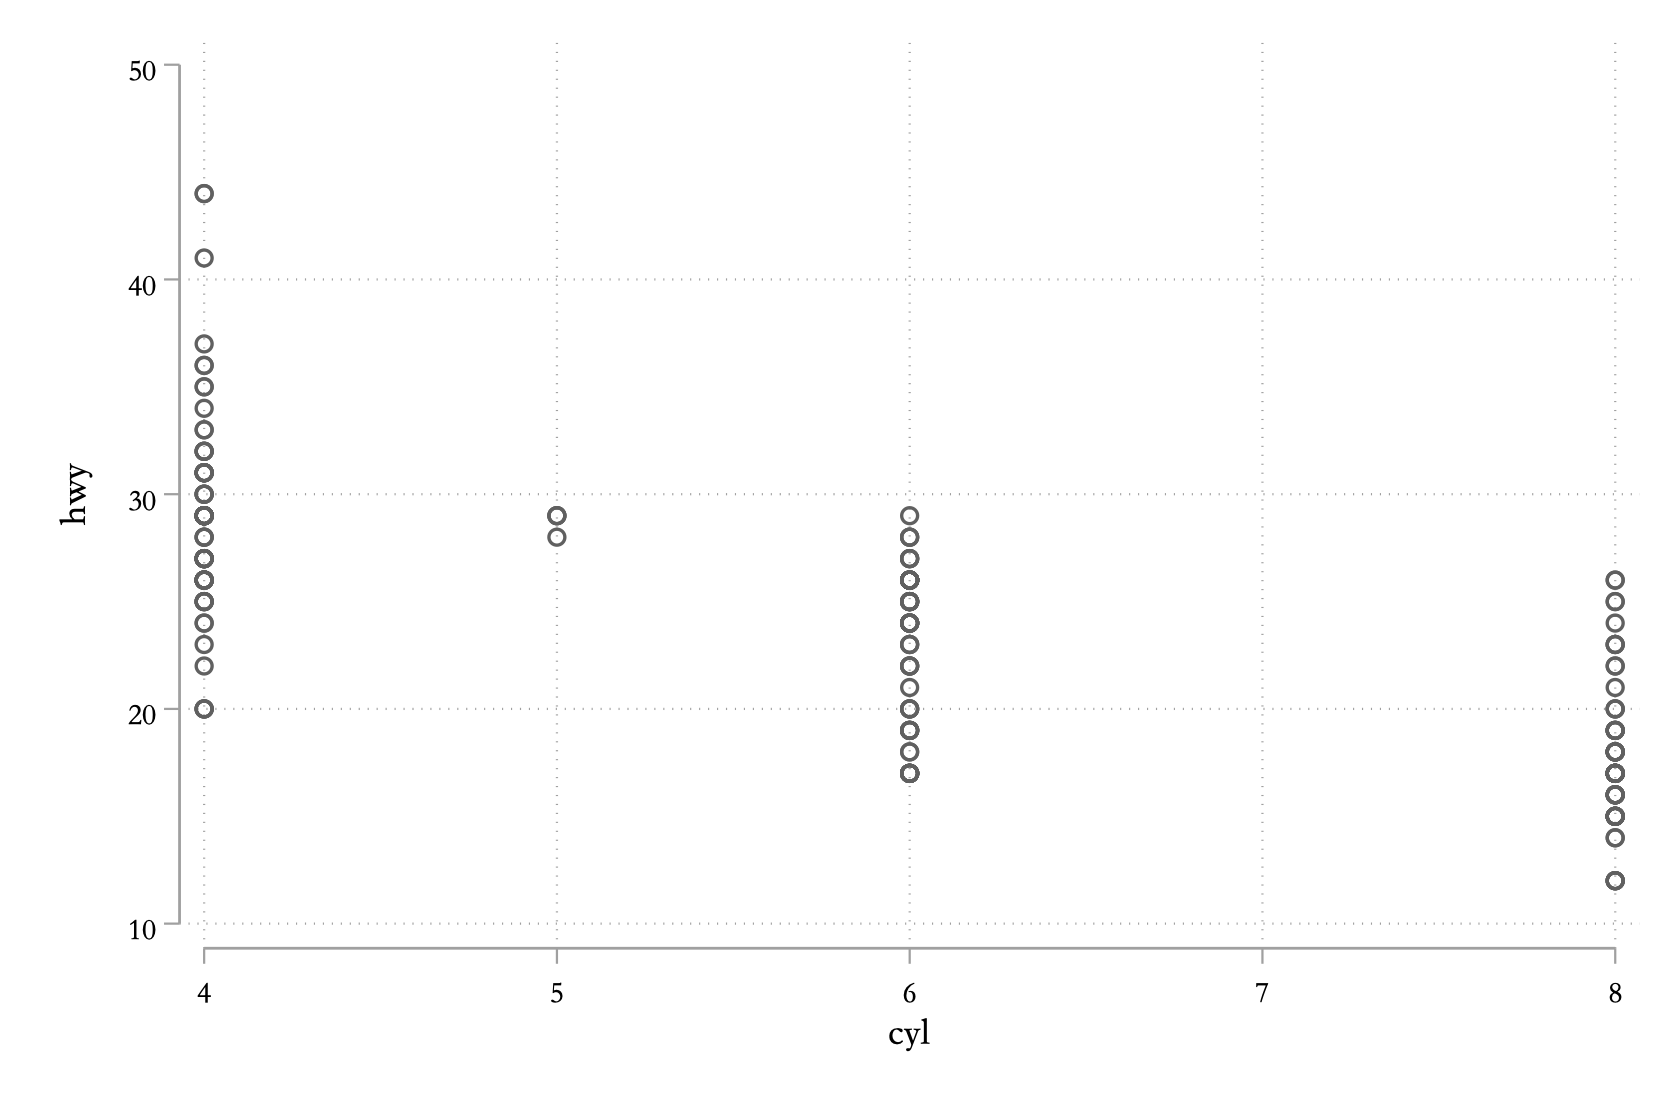
\includegraphics[width=\textwidth]{assets/hwycyl.png}
    \caption{hwy 和 cyl 的关系}
    \label{fig:hwycyl}
  \end{figure}
\end{solution}

\begin{exercise}
  如果你绘制 class 变量和 drv 变量的散点图会发生什么?为什么?
\end{exercise}

\begin{solution}
  \begin{lstlisting}
  sc class drv
  *> string variables not allowed in varlist;
  *> class is a string variable
  *> r(109);
  \end{lstlisting}

  这是因为 Stata 绘图中,字符串变量无法直接被转换成数值变量,所以不能直接用于绘图,所以我们需要首先把字符串变量转换成数值变量再进行绘图,如图 \ref{fig:classnumdrvnum}:

  \begin{lstlisting}
  encode class, gen(classnum) label(class)
  encode drv, gen(drvnum) label(drv)
  sc classnum drvnum
  \end{lstlisting}

  \begin{figure}[htbp]
    \centering
    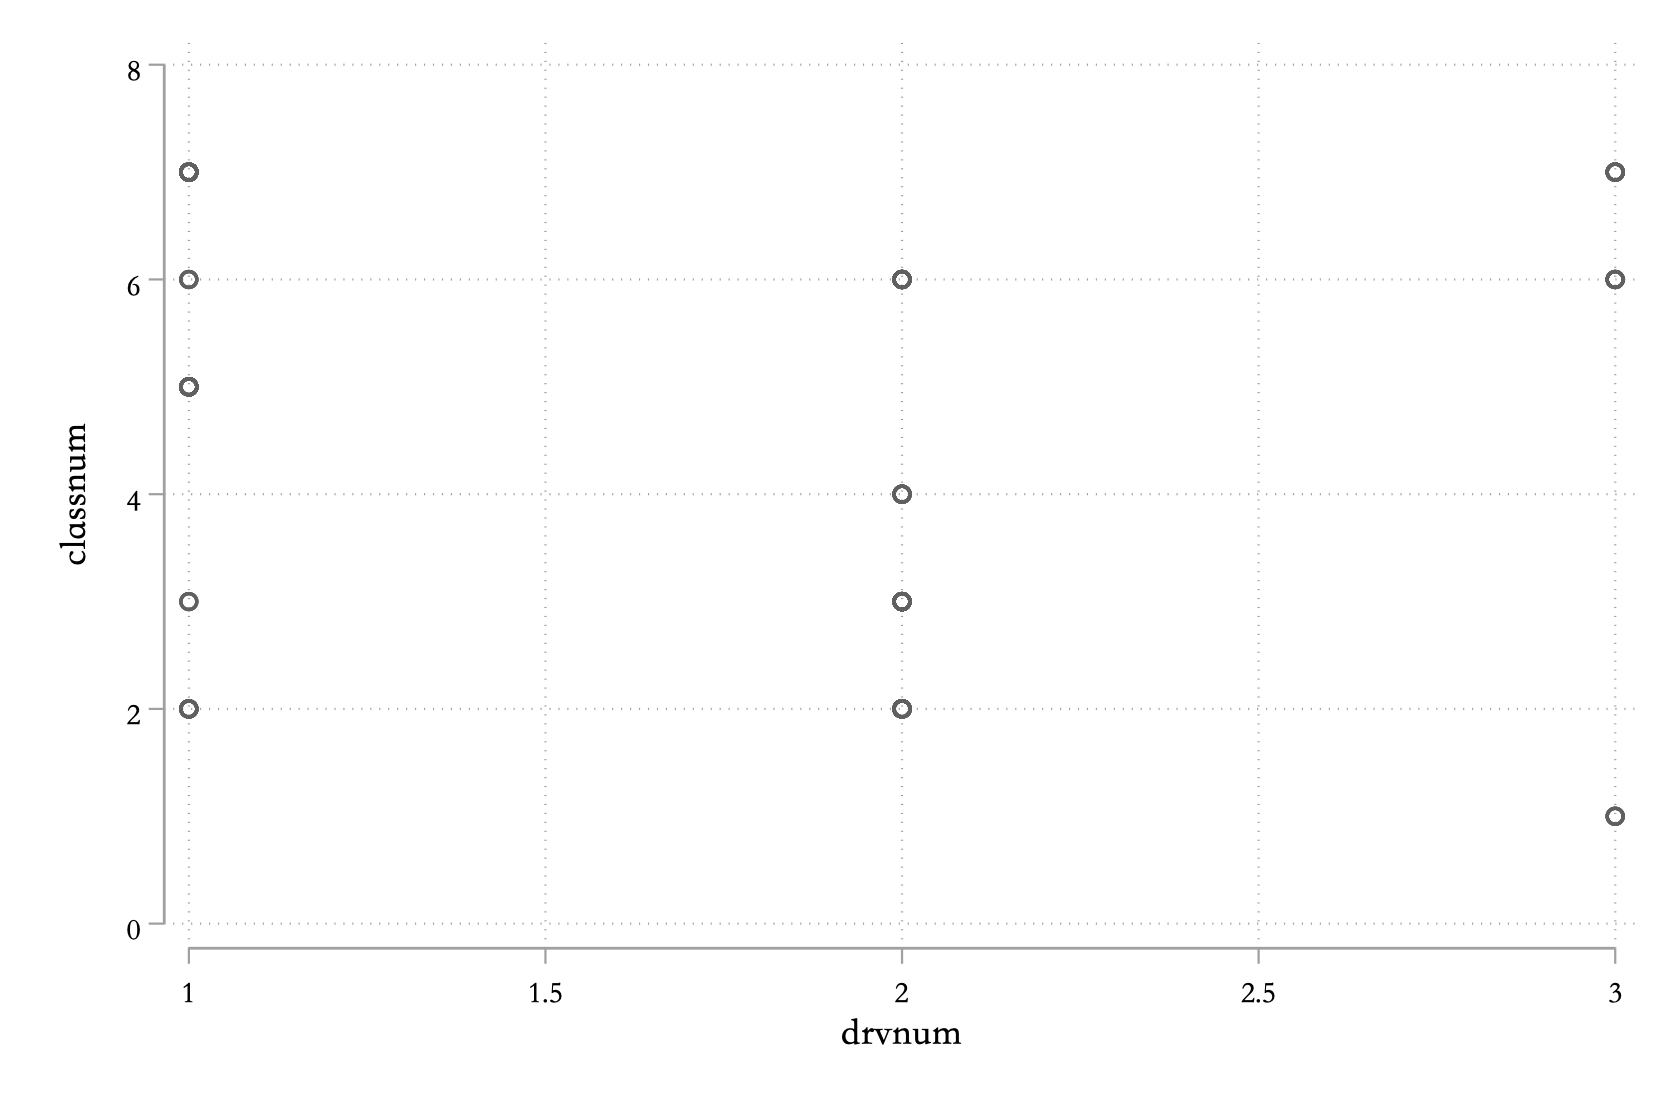
\includegraphics[width=\textwidth]{assets/classnumdrvnum.png}
    \caption{class 和 drv 的关系}
    \label{fig:classnumdrvnum}
  \end{figure}

  我们还可以使用变量的赋值标签作为轴标签,如图 \ref{fig:classnumdrvnum2}:

  \begin{lstlisting}
  sc classnum drvnum, xlab(1 2 3, val) ylab(, val)
  \end{lstlisting}

  \begin{figure}[htbp]
    \centering
    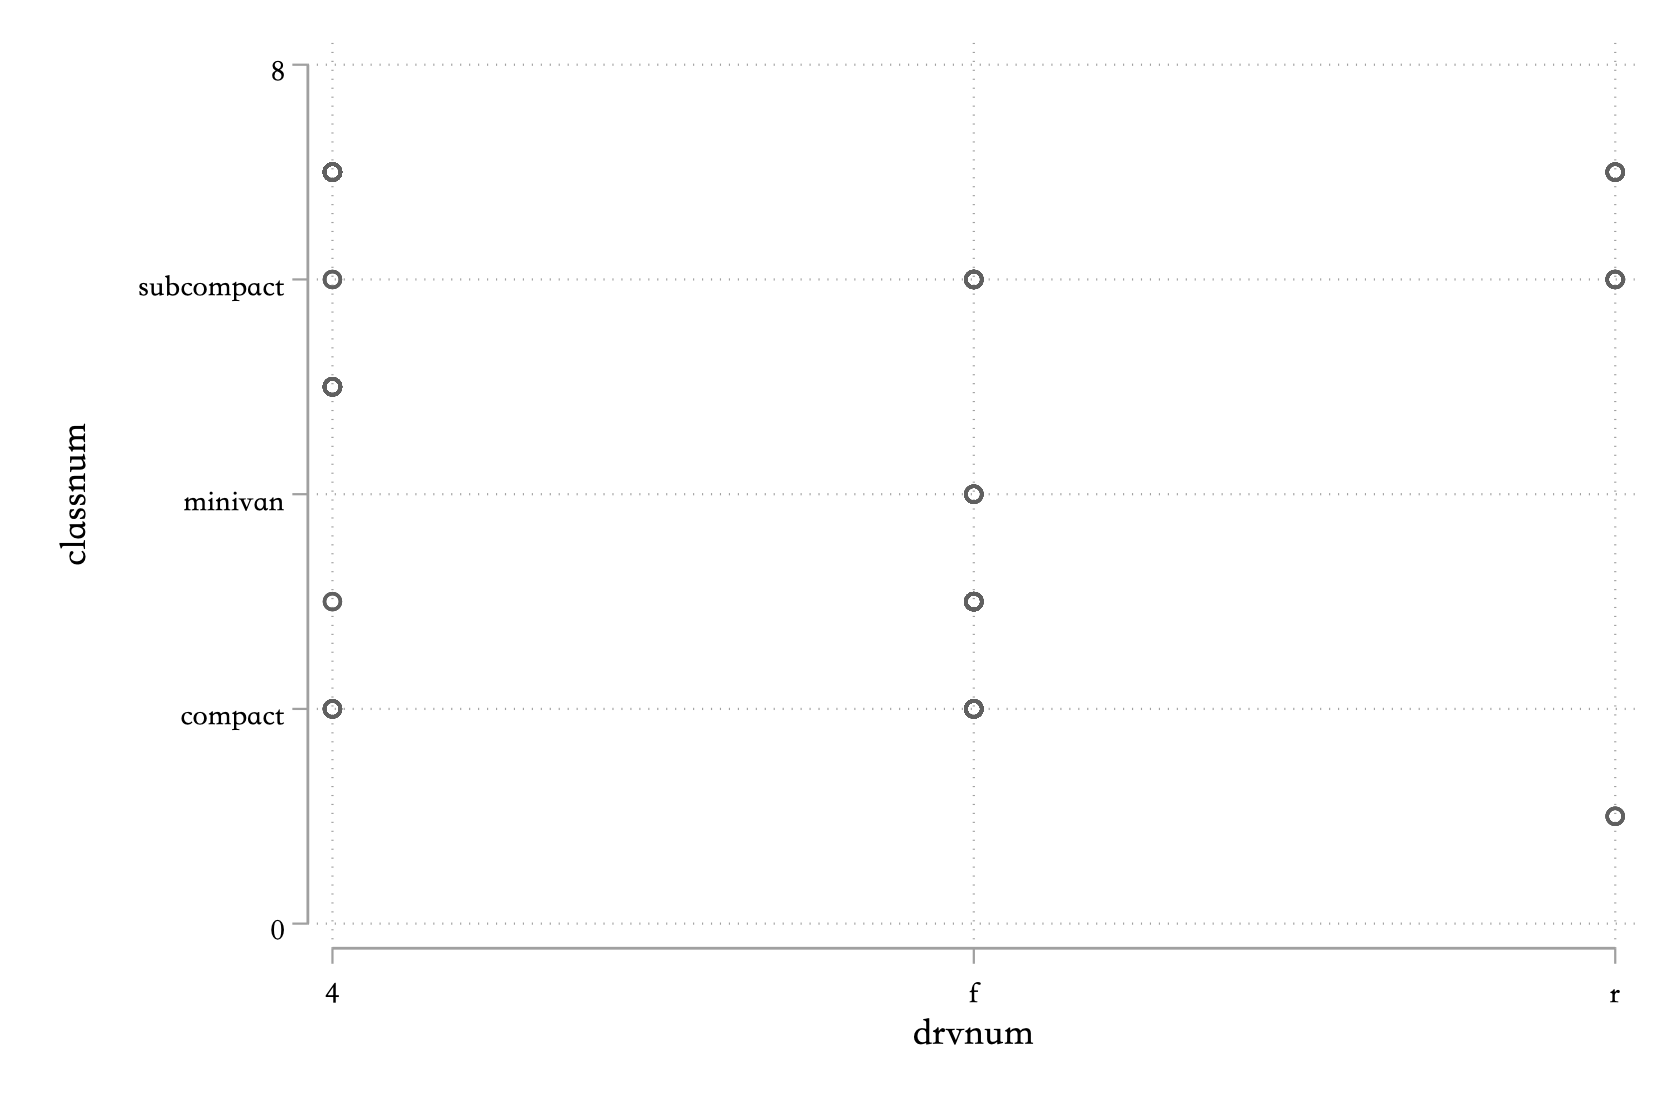
\includegraphics[width=\textwidth]{assets/classnumdrvnum2.png}
    \caption{class 和 drv 的关系}
    \label{fig:classnumdrvnum2}
  \end{figure}

  这里使用了两个选项,xlab() 选项用于控制 x 轴的标签,\texttt{1 2 3} 表示 x 轴上只显示 \texttt{1 2 3} 三个标签,对应的赋值标签正好是 \texttt{4 f r}。val 是 xlab() 选项的选项,所以它的前面用逗号隔开,表示使用赋值标签作为轴标签。
\end{solution}

\section{散点图进阶}
\begin{quote}
``The greatest value of a picture is when it forces us to notice what we never expected to see.'' --- John Tukey
\end{quote}

在图 \ref{fig:hwydispl2} 中,用红色突出的点似乎超过了线性趋势,这些车的里程数高于我们的预期,这是为什么?

\begin{lstlisting}
tw ///
sc hwy displ if displ < 5 | hwy < 22 || ///
sc hwy displ if displ > 5 & hwy > 22, mc(red) ||, ///
leg(off)
\end{lstlisting}

\begin{figure}[htbp]
  \centering
  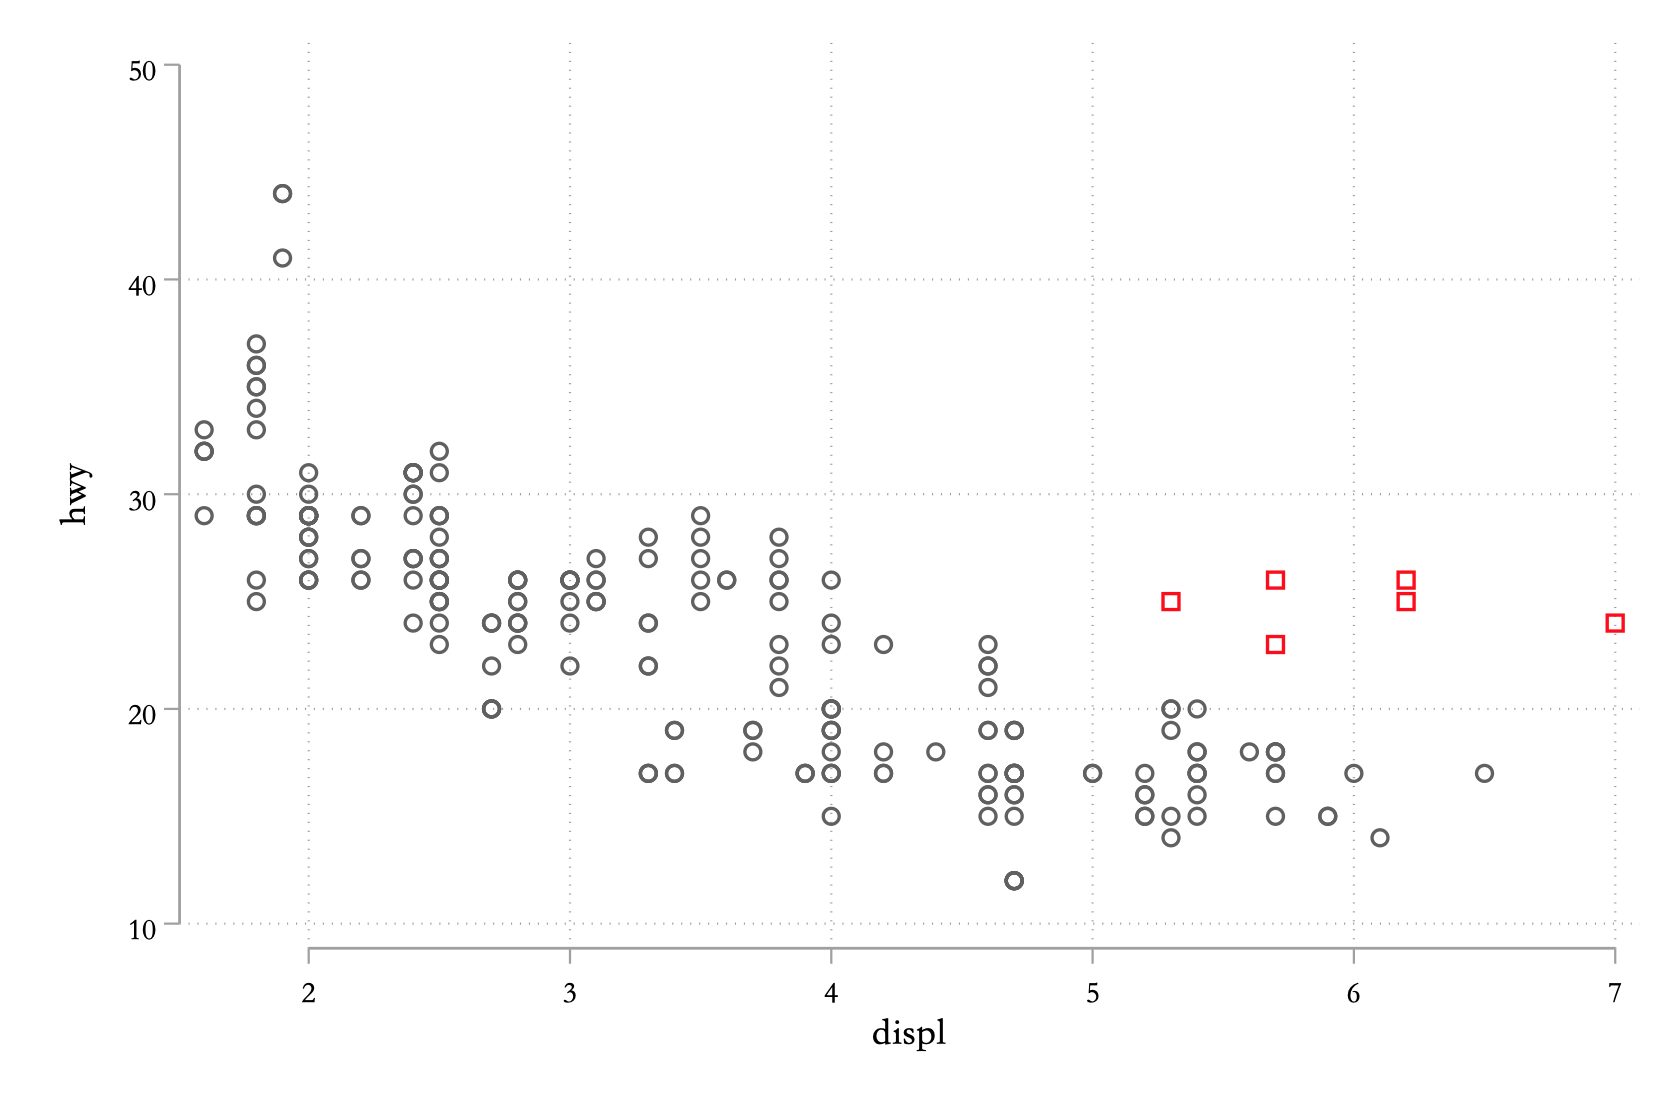
\includegraphics[width=\textwidth]{assets/hwydispl2.png}
  \caption{排量与燃油效率关系中的一些异常值}
  \label{fig:hwydispl2}
\end{figure}

这些异常值出现的一个可能的原因就是这些车中有混合动力车,检验这一猜想的办法就是查看每个 class 的 hwy,如图 \ref{fig:hwydispl3}:

\begin{lstlisting}
* 查看 class 有哪些值
levelsof class
* 可以使用 local() 选项将这些值存储为一个 local 变量
levelsof class, local(class)
* 我们可以针对 class 的每一个值绘制一个图层:
tw ///
sc hwy displ if class == "2seater" || ///
sc hwy displ if class == "compact" || ///
sc hwy displ if class == "midsize" || ///
sc hwy displ if class == "minivan" || ///
sc hwy displ if class == "pickup" || ///
sc hwy displ if class == "subcompact" || ///
sc hwy displ if class == "suv" ||, ///
leg(order(1 "2seater" ///
          2 "compact" ///
          3 "midsize" ///
          4 "minivan" ///
          5 "pickup" ///
          6 "subcompact" ///
          7 "suv") title(class))
\end{lstlisting}

\begin{figure}[htbp]
  \centering
  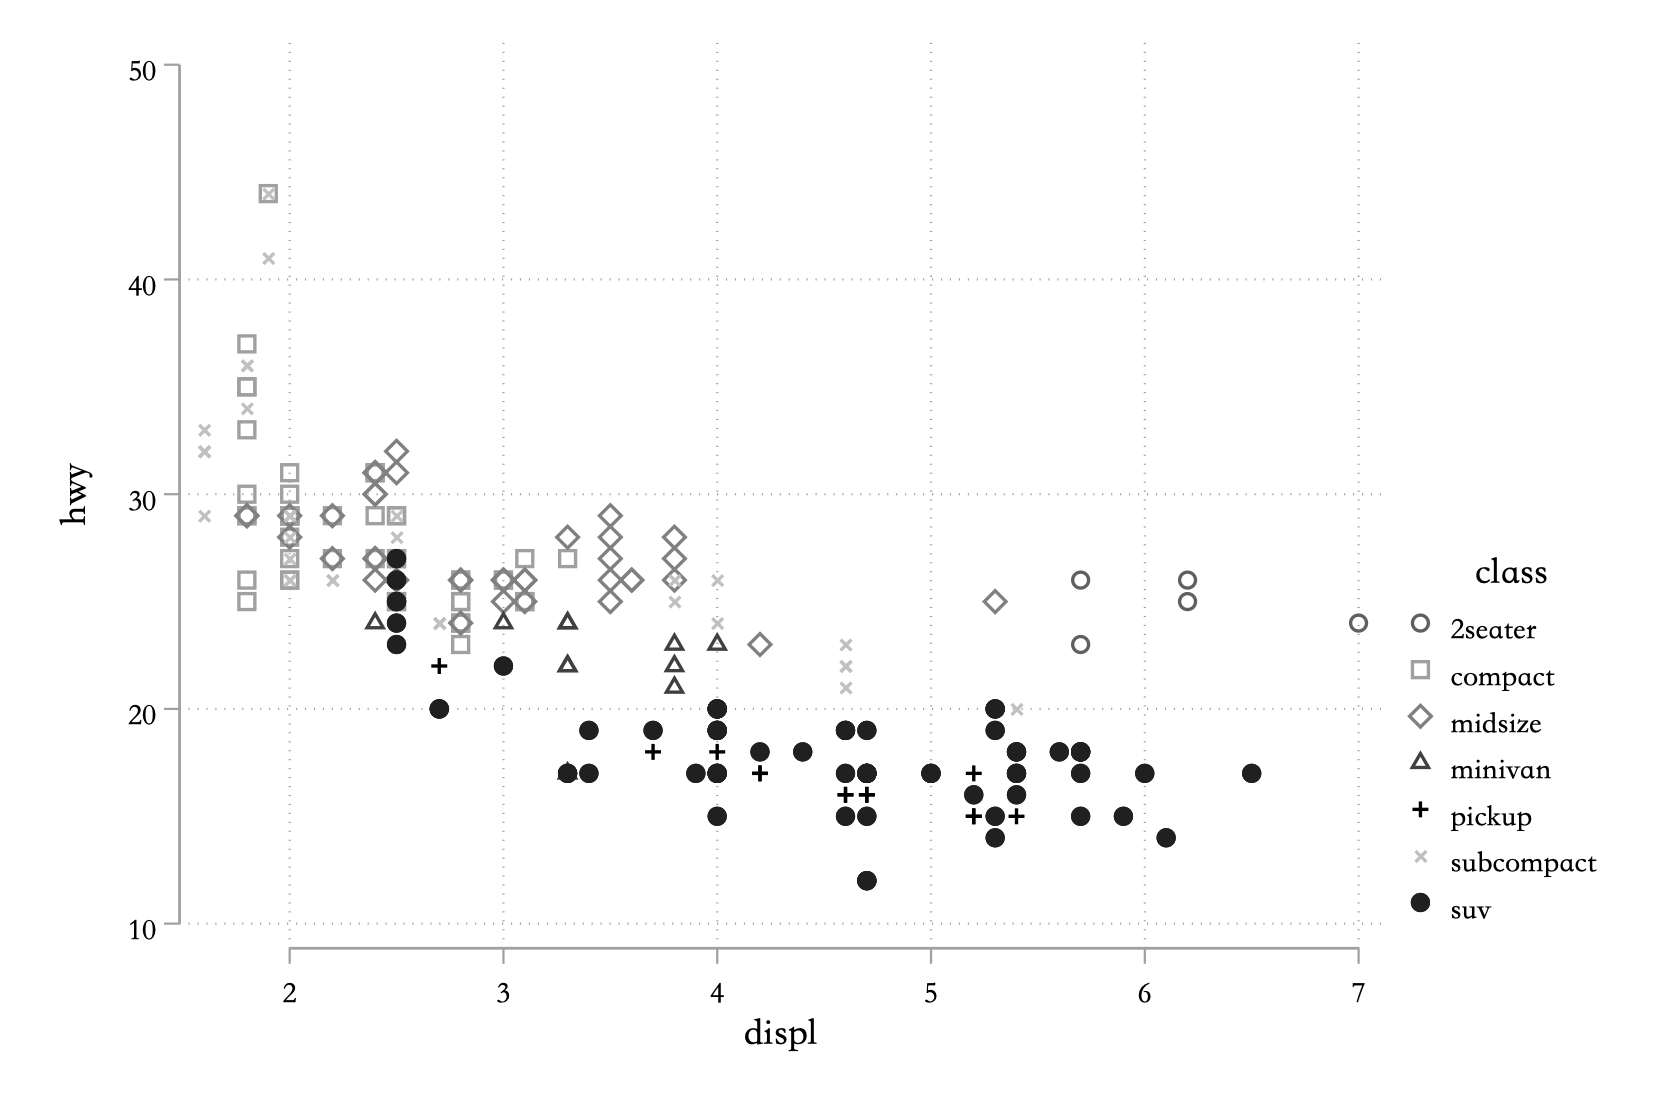
\includegraphics[width=\textwidth]{assets/hwydispl3.png}
  \caption{不同类型汽车排量与燃油效率的关系}
  \label{fig:hwydispl3}
\end{figure}

这里使用不同的散点样式表示不同图层,当然我们也可以使用不同的颜色表示,\lstinline{colorscheme} 命令是个非常好用的调色选色命令,其调色板来源于: \href{http://colorbrewer2.org/}{ColorBrewer: Color Advice for Maps},安装方式如下:

\begin{lstlisting}
net install colorscheme.pkg, from("https://github.com/matthieugomez/stata-colorscheme/raw/master/")
\end{lstlisting}

关于这个命令的使用,你可以参考其帮助文档(help colorscheme)或者我的博客文章: \href{https://www.czxa.top/posts/16049/}{colorscheme——调色选色命令}。

我最喜欢的是 \texttt{Paired} 配色方案,如图 \ref{fig:Paired}:

\begin{lstlisting}
colorscheme 12, palette(Paired) display
return list
*> macros:
*>     r(color1) : "166 206 227"
*>     r(color2) : "031 120 180"
*>     r(color3) : "178 223 138"
*>     r(color4) : "051 160 044"
*>     r(color5) : "251 154 153"
*>     r(color6) : "227 026 028"
*>     r(color7) : "253 191 111"
*>     r(color8) : "255 127 000"
*>     r(color9) : "202 178 214"
*>    r(color10) : "106 061 154"
*>    r(color11) : "255 255 153"
*>    r(color12) : "177 089 040"
*>     r(colors) : ""166 206 227" "031 120 180"  "178 223 138"  "051 160 044.."
\end{lstlisting}

\begin{figure}[htbp]
  \centering
  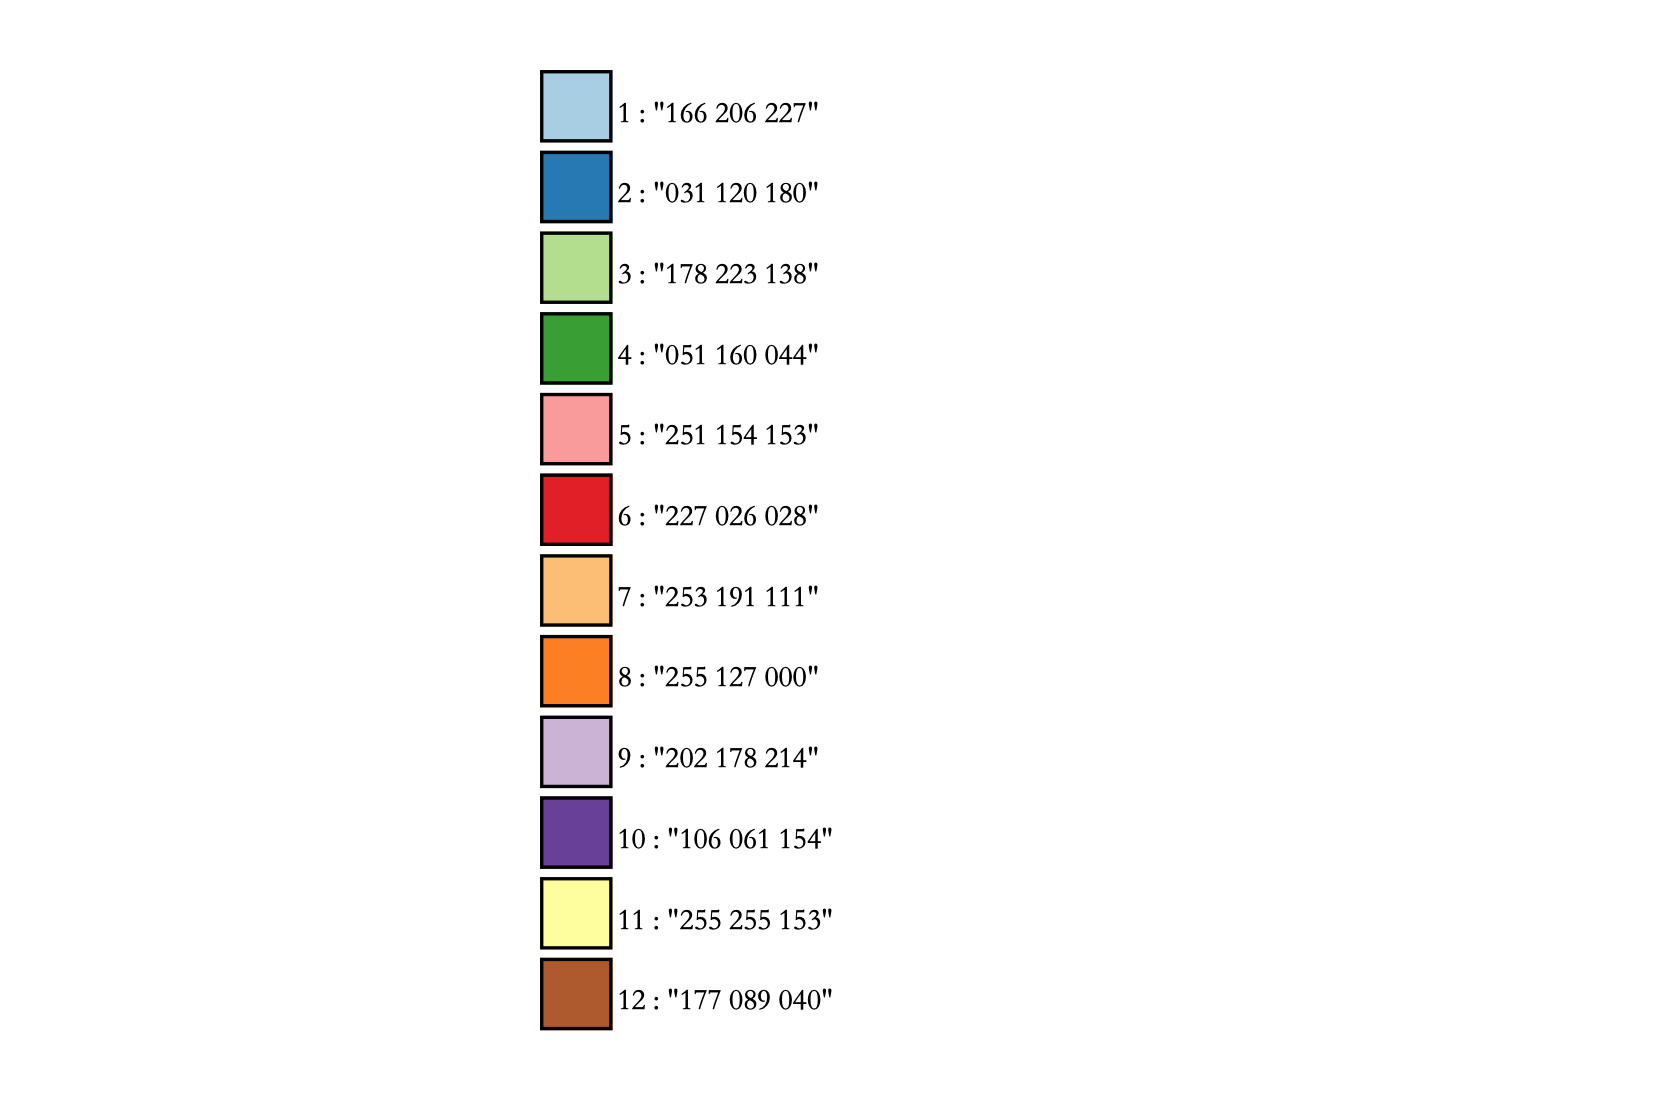
\includegraphics[width=\textwidth]{assets/Paired.png}
  \caption{Paired 配色方案}
  \label{fig:Paired}
\end{figure}

这里我们需要 7 种颜色,如图 \ref{fig:hwydispl4}:

\begin{lstlisting}
colorscheme 7, palette(Paired)
tw ///
sc hwy displ if class == "2seater", mc("`r(color1)'") ms(o) || ///
sc hwy displ if class == "compact", mc("`r(color2)'") ms(o) || ///
sc hwy displ if class == "midsize", mc("`r(color3)'") ms(o) || ///
sc hwy displ if class == "minivan", mc("`r(color4)'") ms(o) || ///
sc hwy displ if class == "pickup", mc("`r(color5)'") ms(o) || ///
sc hwy displ if class == "subcompact", mc("`r(color6)'") ms(o) || ///
sc hwy displ if class == "suv", mc("`r(color7)'") ms(o) ||, ///
leg(order(1 "2seater" ///
          2 "compact" ///
          3 "midsize" ///
          4 "minivan" ///
          5 "pickup" ///
          6 "subcompact" ///
          7 "suv") title(class))
\end{lstlisting}

\begin{figure}[htbp]
  \centering
  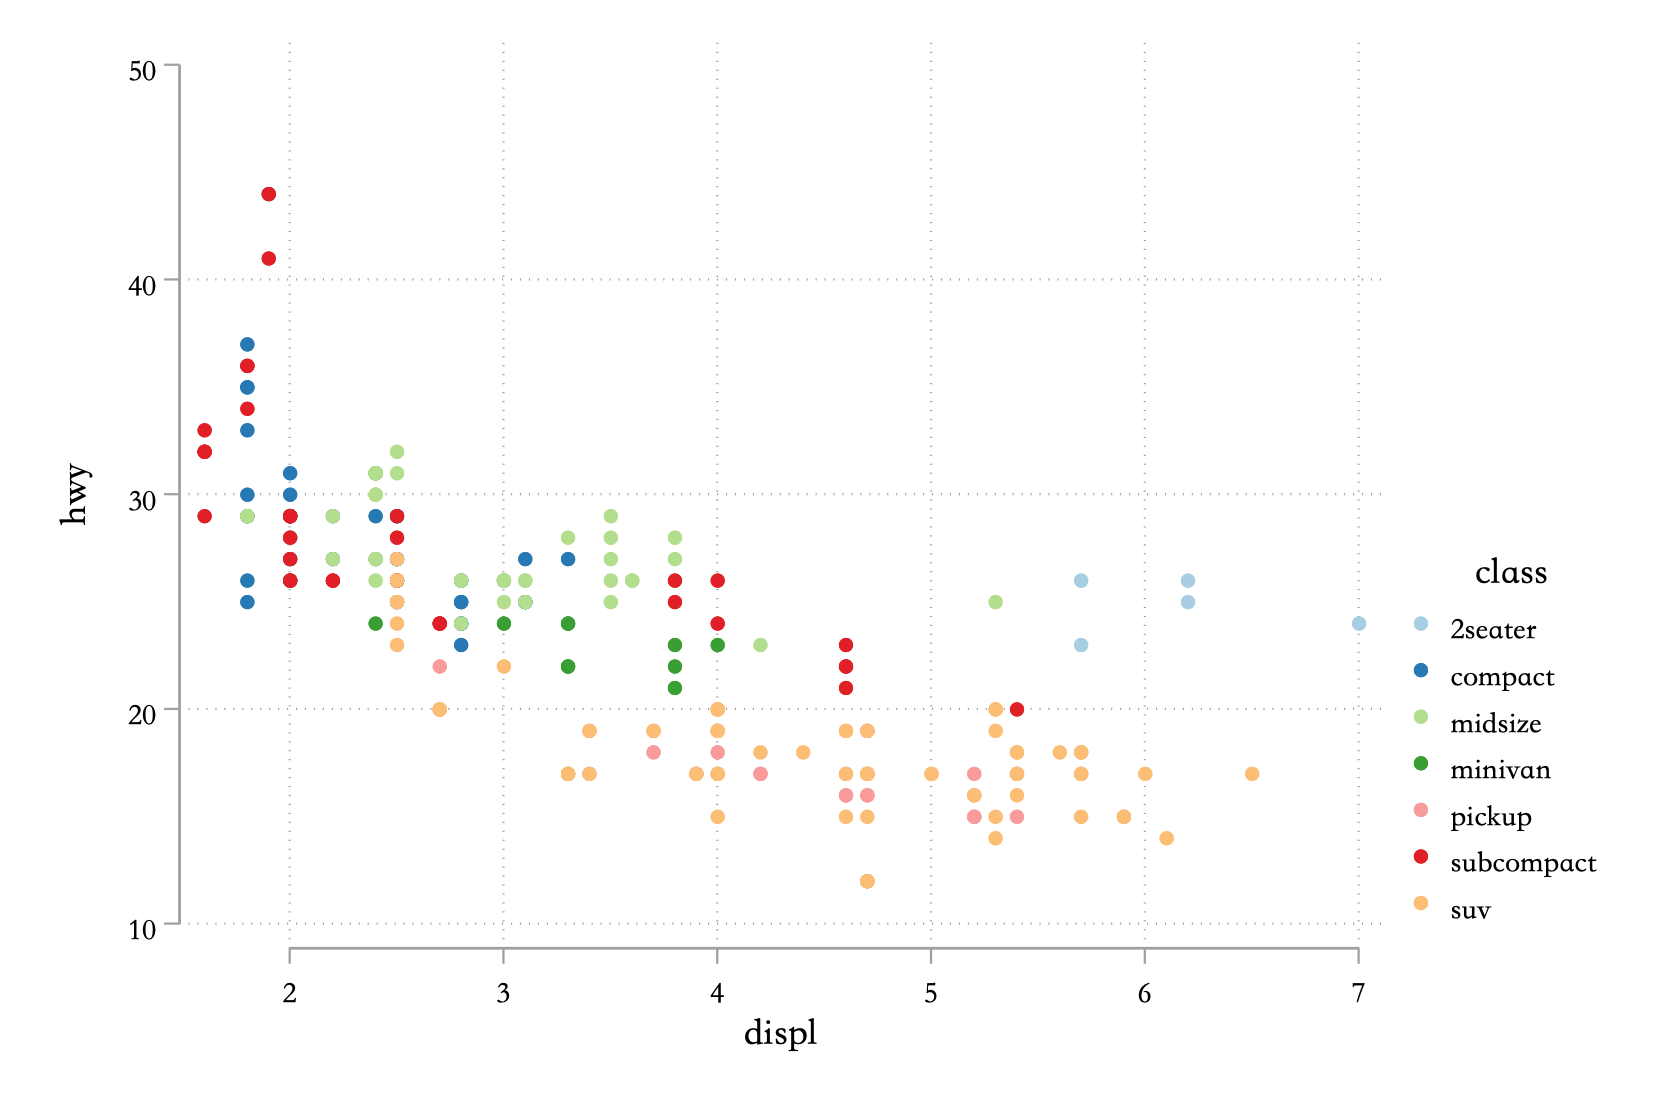
\includegraphics[width=\textwidth]{assets/hwydispl4.png}
  \caption{不同类型汽车排量与燃油效率的关系}
  \label{fig:hwydispl4}
\end{figure}

当然你也可以用散点的大小表示不同的图层,如图 \ref{fig:hwydispl5}:

\begin{lstlisting}
colorscheme 7, palette(Set2)
tw ///
sc hwy displ if class == "2seater", mc("`r(color1)'") ms(o) msize(*1) || ///
sc hwy displ if class == "compact", mc("`r(color2)'") ms(o) msize(*1.5) || ///
sc hwy displ if class == "midsize", mc("`r(color3)'") ms(o) msize(*2) || ///
sc hwy displ if class == "minivan", mc("`r(color4)'") ms(o) msize(*2.5) || ///
sc hwy displ if class == "pickup", mc("`r(color5)'") ms(o) msize(*3) || ///
sc hwy displ if class == "subcompact", mc("`r(color6)'") ms(o) msize(*3.5) || ///
sc hwy displ if class == "suv", mc("`r(color7)'") ms(o) msize(*4) ||, ///
leg(order(1 "2seater" ///
          2 "compact" ///
          3 "midsize" ///
          4 "minivan" ///
          5 "pickup" ///
          6 "subcompact" ///
          7 "suv") title(class))
\end{lstlisting}

\begin{figure}[htbp]
  \centering
  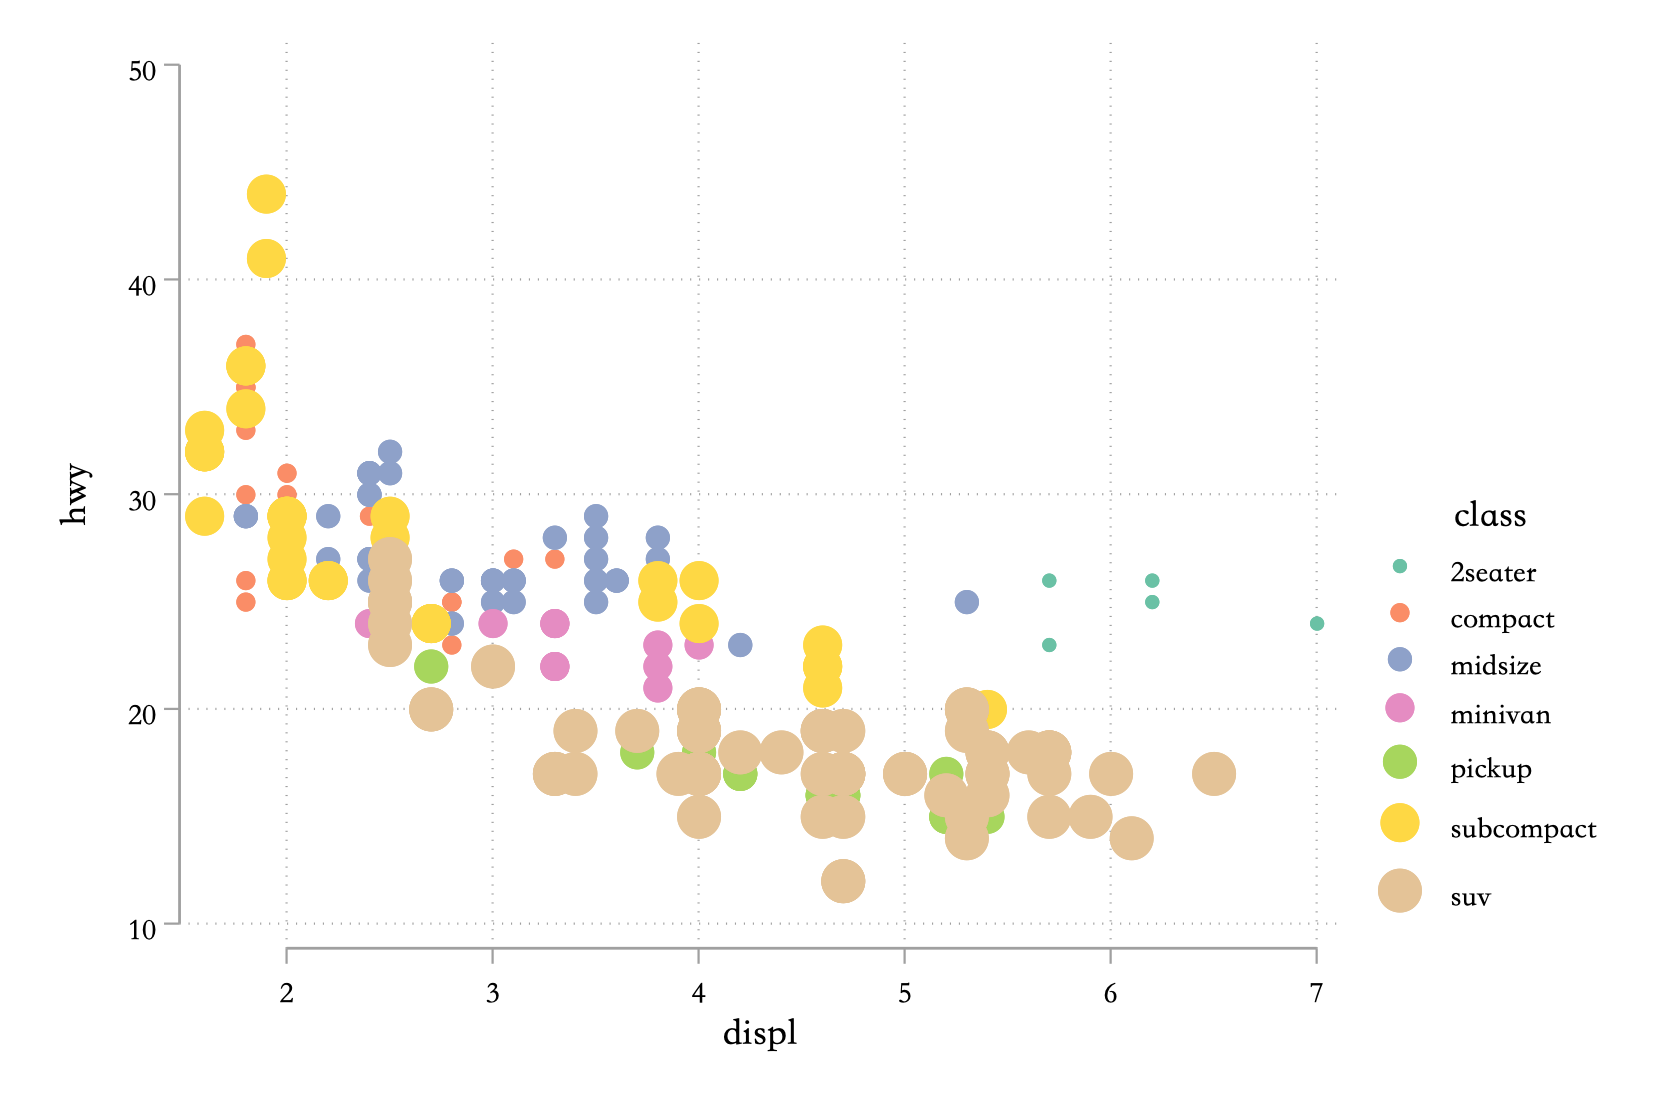
\includegraphics[width=\textwidth]{assets/hwydispl5.png}
  \caption{不同类型汽车排量与燃油效率的关系}\label{fig:hwydispl5}
\end{figure}

最后 Stata15 在绘图方面引入了一个新特性就是可以为图层设置透明度了!关于透明度的使用可以参考 Stata 官网上的相关介绍和我的博客文章: \href{https://www.czxa.top/posts/44086/}{Stata15绘图的新功能:设置图形的透明度},图 \ref{fig:hwydispl6}展示了使用透明度的效果:

\begin{lstlisting}
/* 左图 */
tw ///
sc hwy displ if class == "2seater" || ///
sc hwy displ if class == "compact" || ///
sc hwy displ if class == "midsize" || ///
sc hwy displ if class == "minivan" || ///
sc hwy displ if class == "pickup" || ///
sc hwy displ if class == "subcompact" || ///
sc hwy displ if class == "suv" ||, ///
leg(order(1 "2seater" ///
          2 "compact" ///
          3 "midsize" ///
          4 "minivan" ///
          5 "pickup" ///
          6 "subcompact" ///
          7 "suv") title(class)) name(p1) nodraw
/* 右图 */
tw ///
sc hwy displ if class == "2seater", mc(%90) ms(o) || ///
sc hwy displ if class == "compact", mc(%80) ms(o) || ///
sc hwy displ if class == "midsize", mc(%70) ms(o) || ///
sc hwy displ if class == "minivan", mc(%60) ms(o) || ///
sc hwy displ if class == "pickup", mc(%50) ms(o) || ///
sc hwy displ if class == "subcompact", mc(%40) ms(o) || ///
sc hwy displ if class == "suv", mc(%30) ms(o) ||, ///
leg(order(1 "2seater" ///
          2 "compact" ///
          3 "midsize" ///
          4 "minivan" ///
          5 "pickup" ///
          6 "subcompact" ///
          7 "suv") title(class)) name(p2) nodraw
/* 合并 */
gr combine p1 p2
\end{lstlisting}

\begin{figure}[htbp]
  \centering
  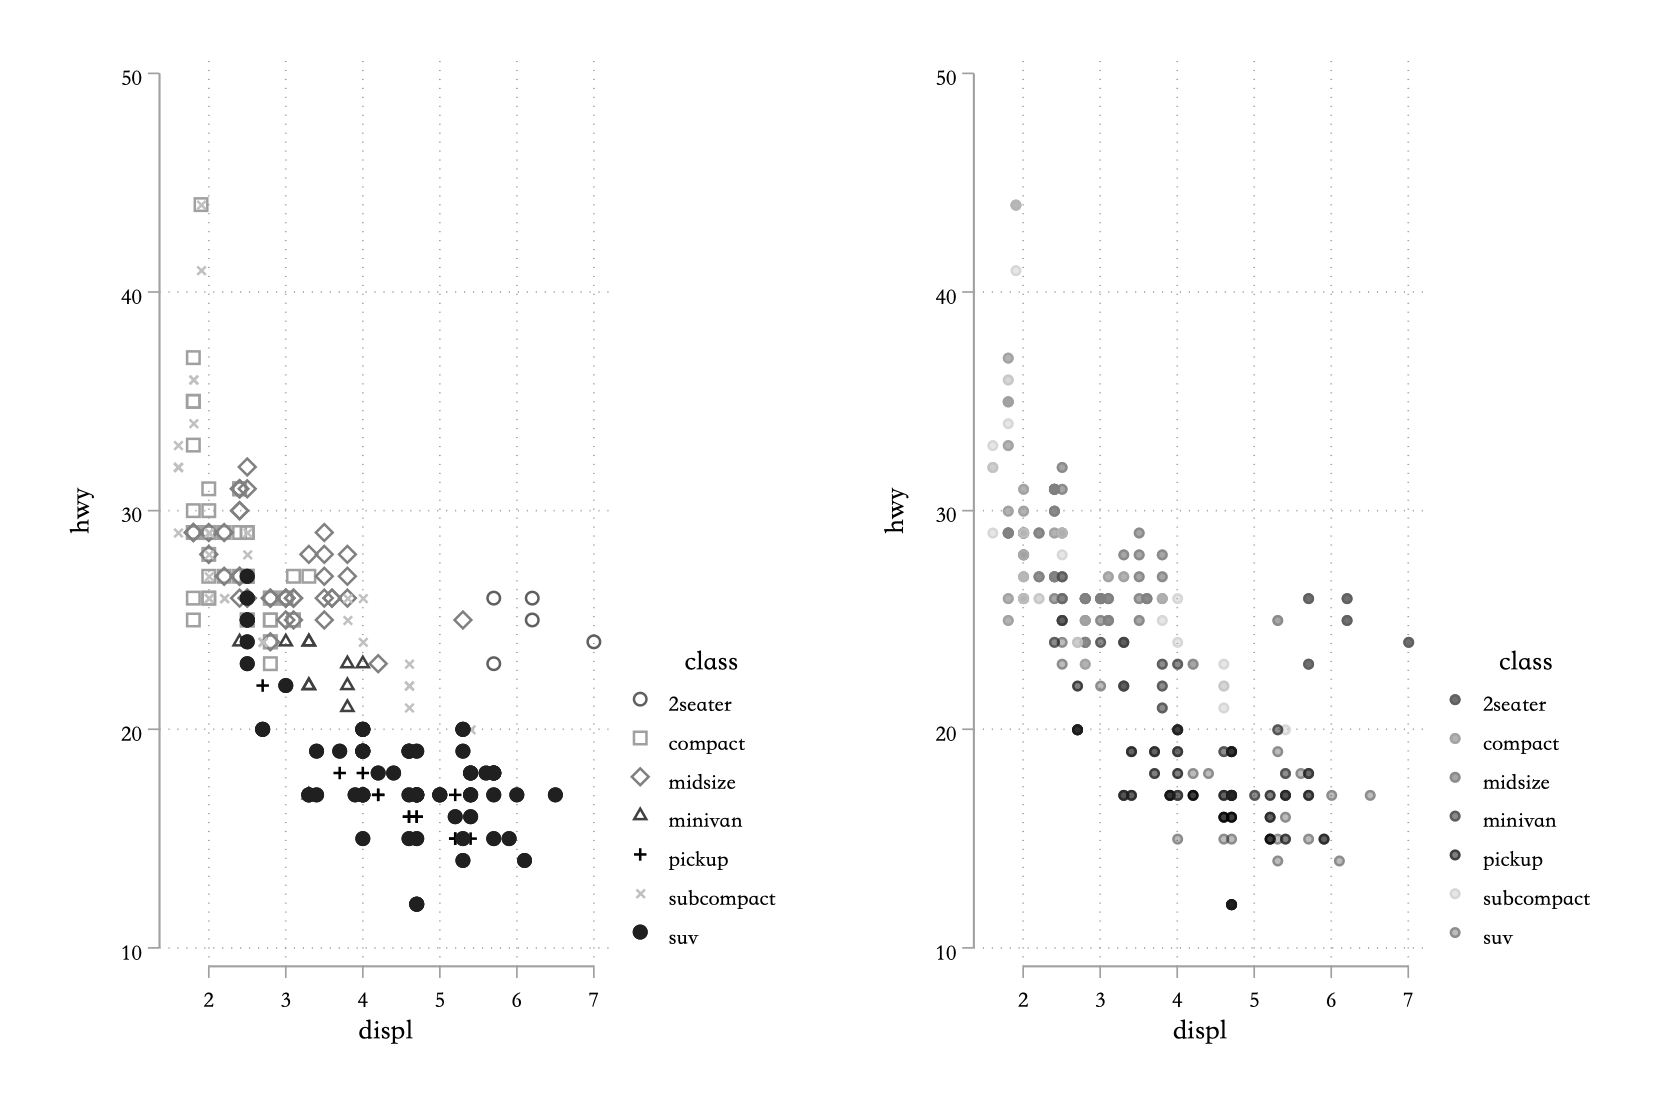
\includegraphics[width=\textwidth]{assets/hwydispl6.png}
  \caption{不同类型汽车排量与燃油效率的关系}
  \label{fig:hwydispl6}
\end{figure}

Stata 绘图中的散点样式如图 \ref{fig:symbolpalette}:

\begin{lstlisting}
palette symbolpalette
\end{lstlisting}

\begin{figure}[htbp]
  \centering
  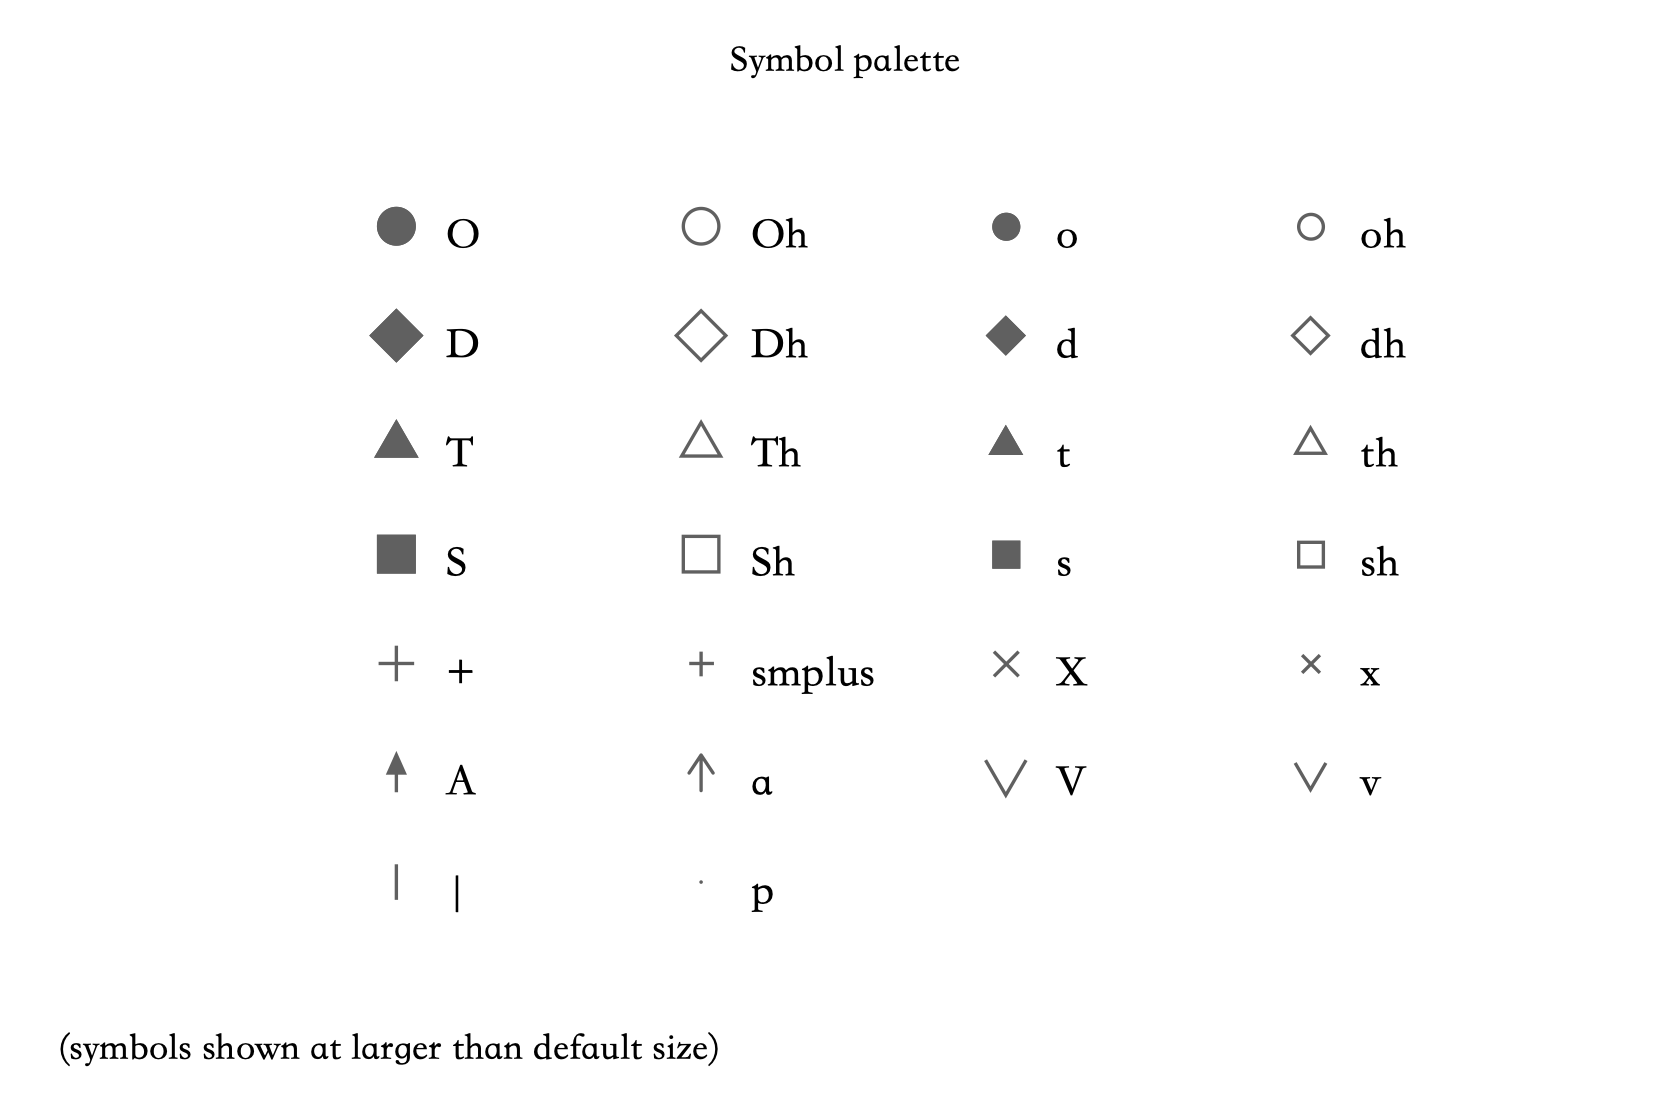
\includegraphics[width=\textwidth]{assets/symbolpalette.png}
  \caption{Stata 绘图中的散点样式}
  \label{fig:symbolpalette}
\end{figure}

\section{分面}

把多个图层叠加在一起就会产生相互重叠的问题,因此我们有时候会选择将不同的图层分开绘制,也就是分面,如图 \ref{fig:hwydisplbyclass}:

\begin{lstlisting}
sc hwy displ, by(class)
\end{lstlisting}

\begin{figure}[htbp]
  \centering
  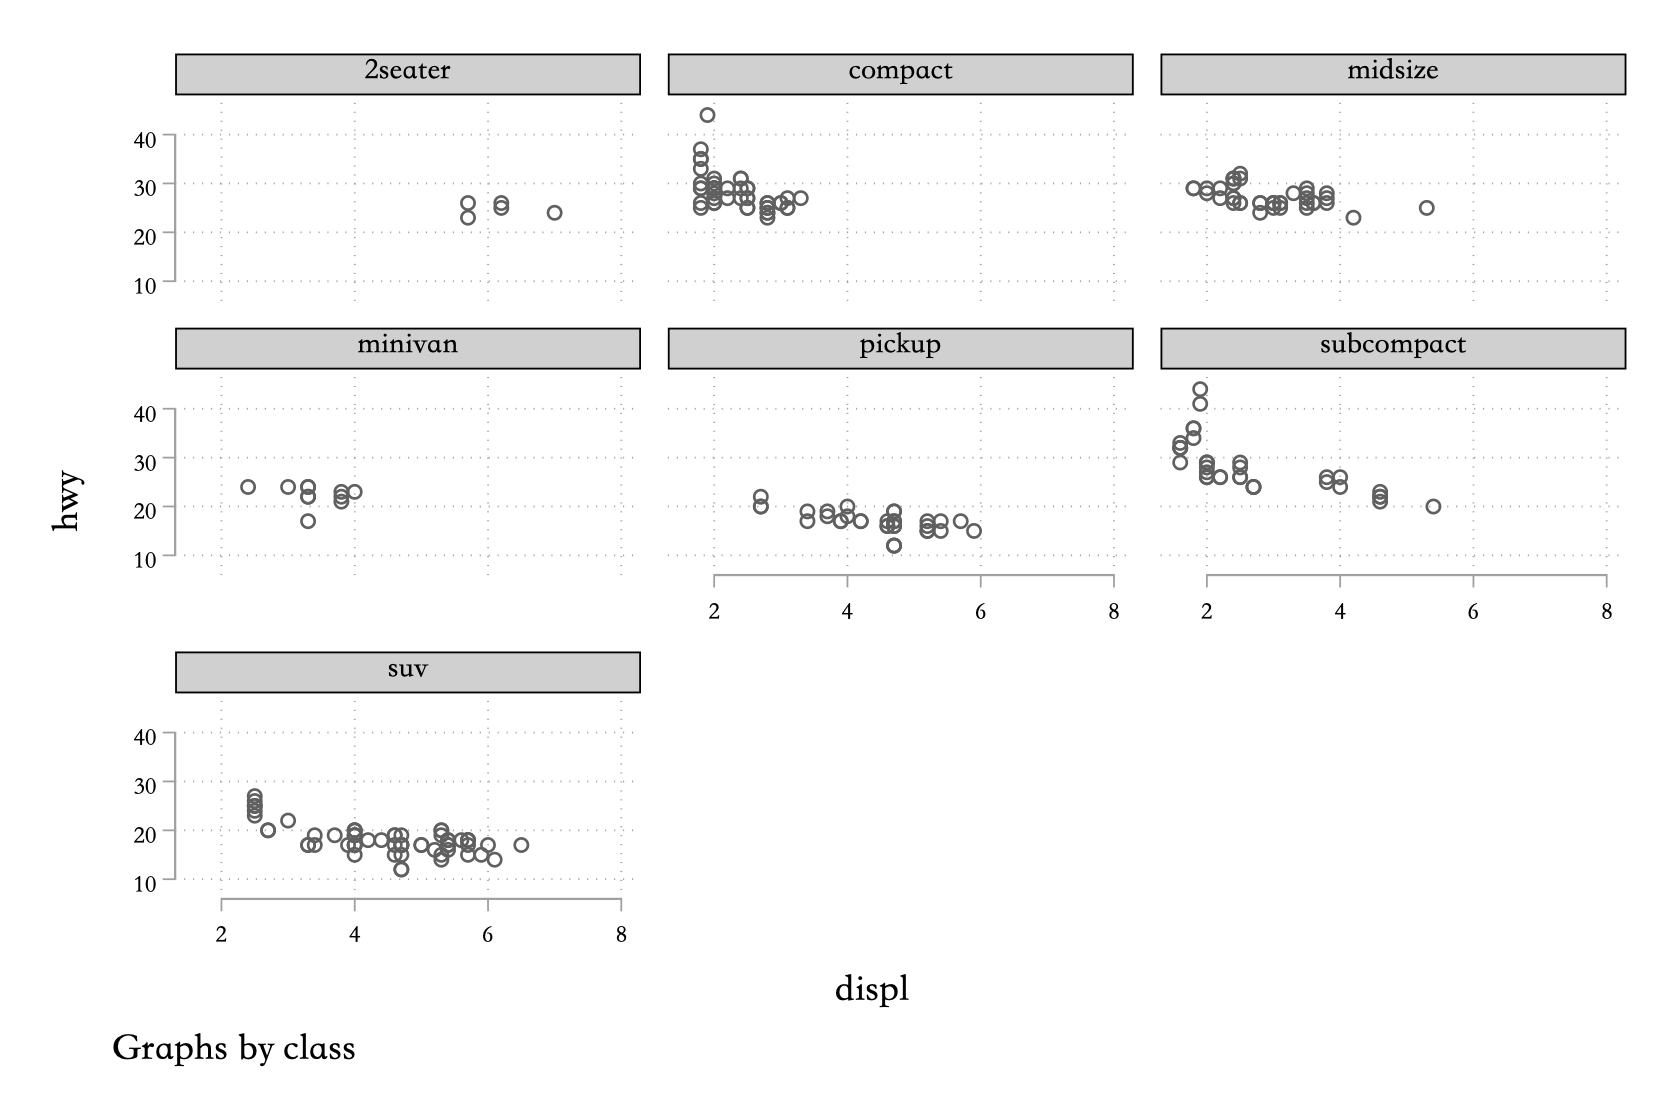
\includegraphics[width=1\textwidth]{assets/hwydisplbyclass.png}
  \caption{不同型号汽车排量与燃油效率的关系}
  \label{fig:hwydisplbyclass}
\end{figure}

我们也可以使用两个变量的组合进行分面,如图 \ref{fig:hwydisplbyfrvcyl}:

\begin{lstlisting}
sc hwy displ, by(drv cyl)
\end{lstlisting}

\begin{figure}[htbp]
  \centering
  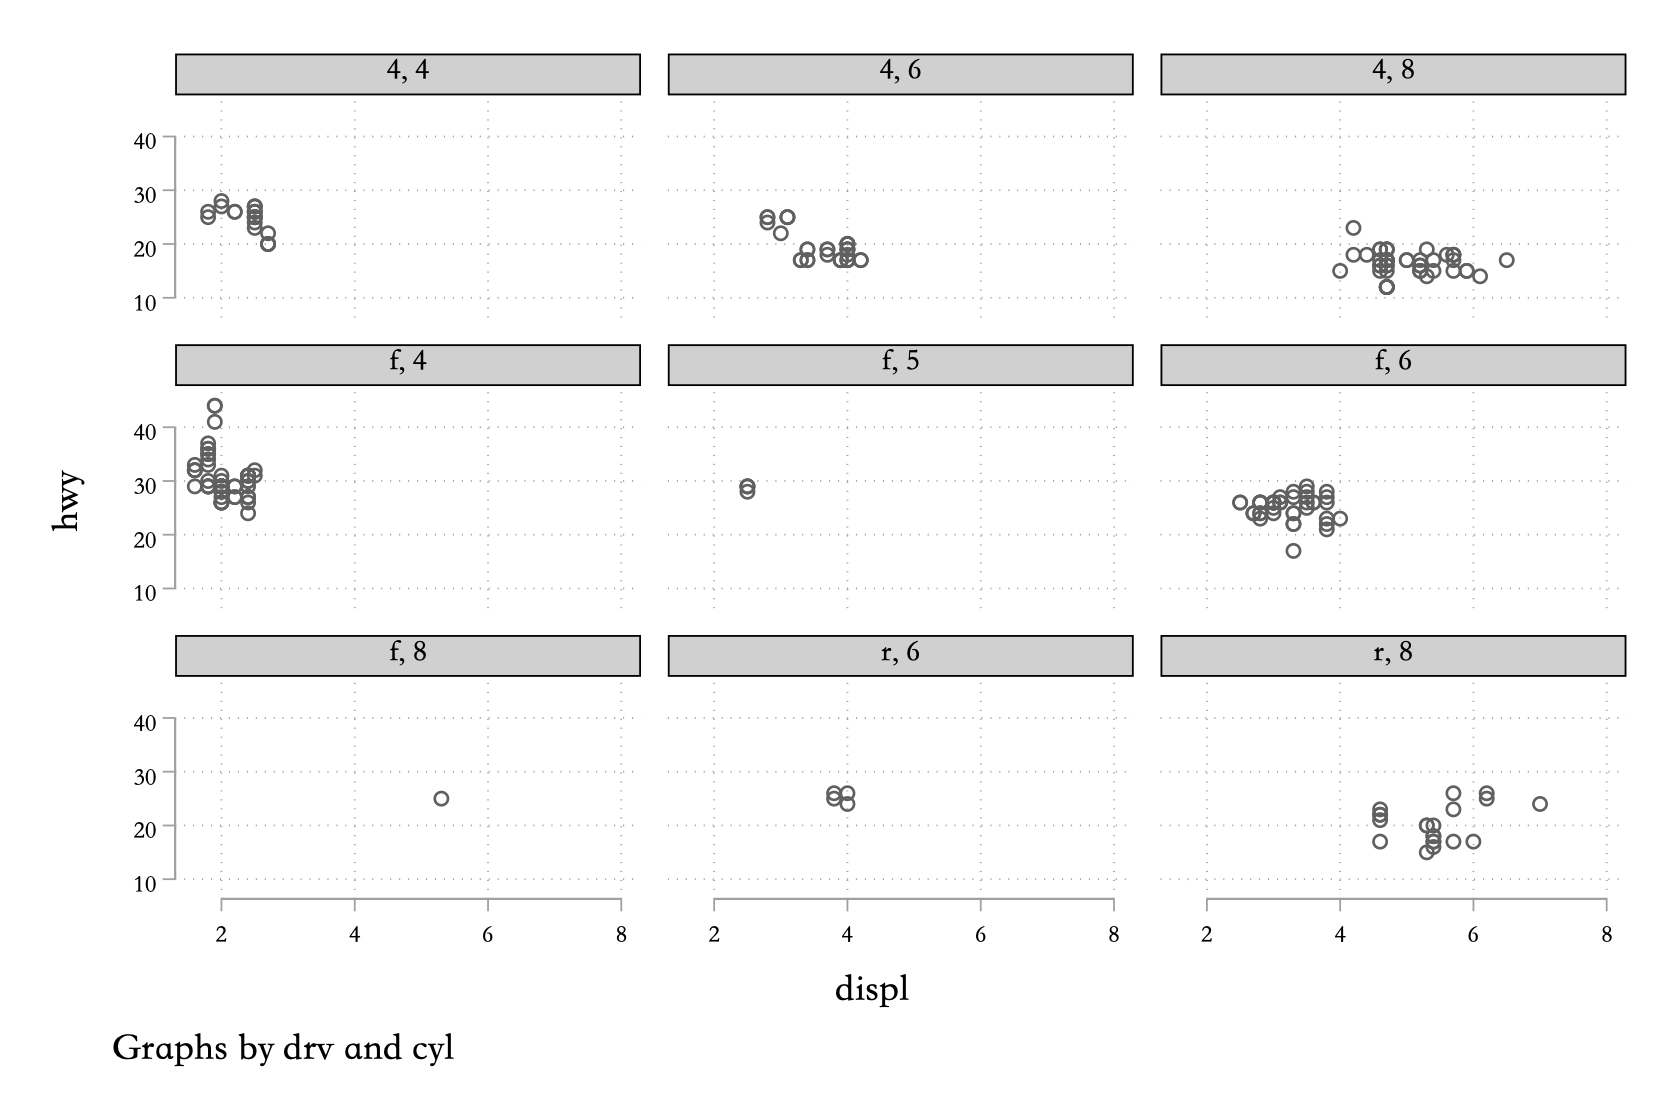
\includegraphics[width=1\textwidth]{assets/hwydisplbyfrvcyl.png}
  \caption{不同drv和cyl的汽车排量与燃油效率的关系}
  \label{fig:hwydisplbyfrvcyl}
\end{figure}

我们还可以自定义分面图的排列,例如全部排列在一行,如图 \ref{fig:hwydisplbyclass2}:

\begin{lstlisting}
sc hwy displ, by(class, row(1))
\end{lstlisting}

\begin{figure}[htbp]
  \centering
  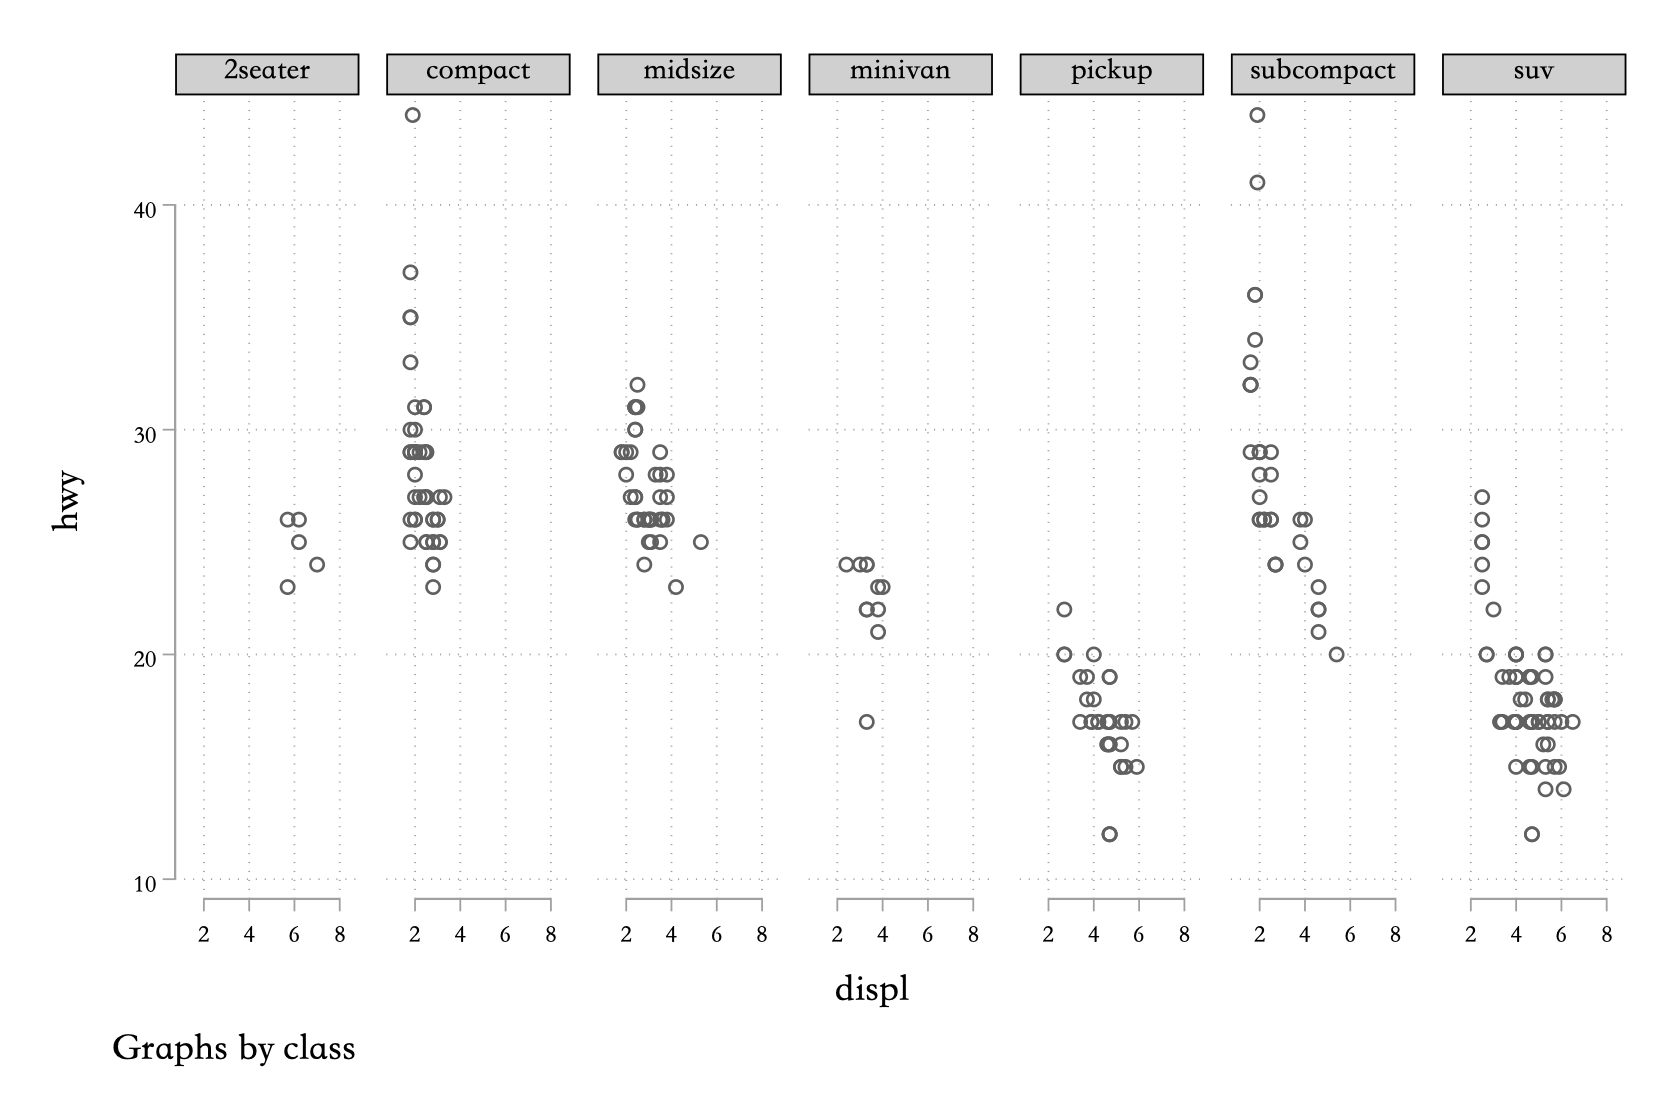
\includegraphics[width=1\textwidth]{assets/hwydisplbyclass2.png}
  \caption{不同型号汽车排量与燃油效率的关系}\label{fig:hwydisplbyclass2}
\end{figure}

经常有小伙伴在绘制分面图的时候想把左下角的 \texttt{Graphs\ by\ xx} 去掉,这个可以通过 \texttt{by()} 的子选项去除:

\begin{lstlisting}
sc hwy displ, by(class, note(""))
\end{lstlisting}

\begin{figure}[htbp]
  \centering
  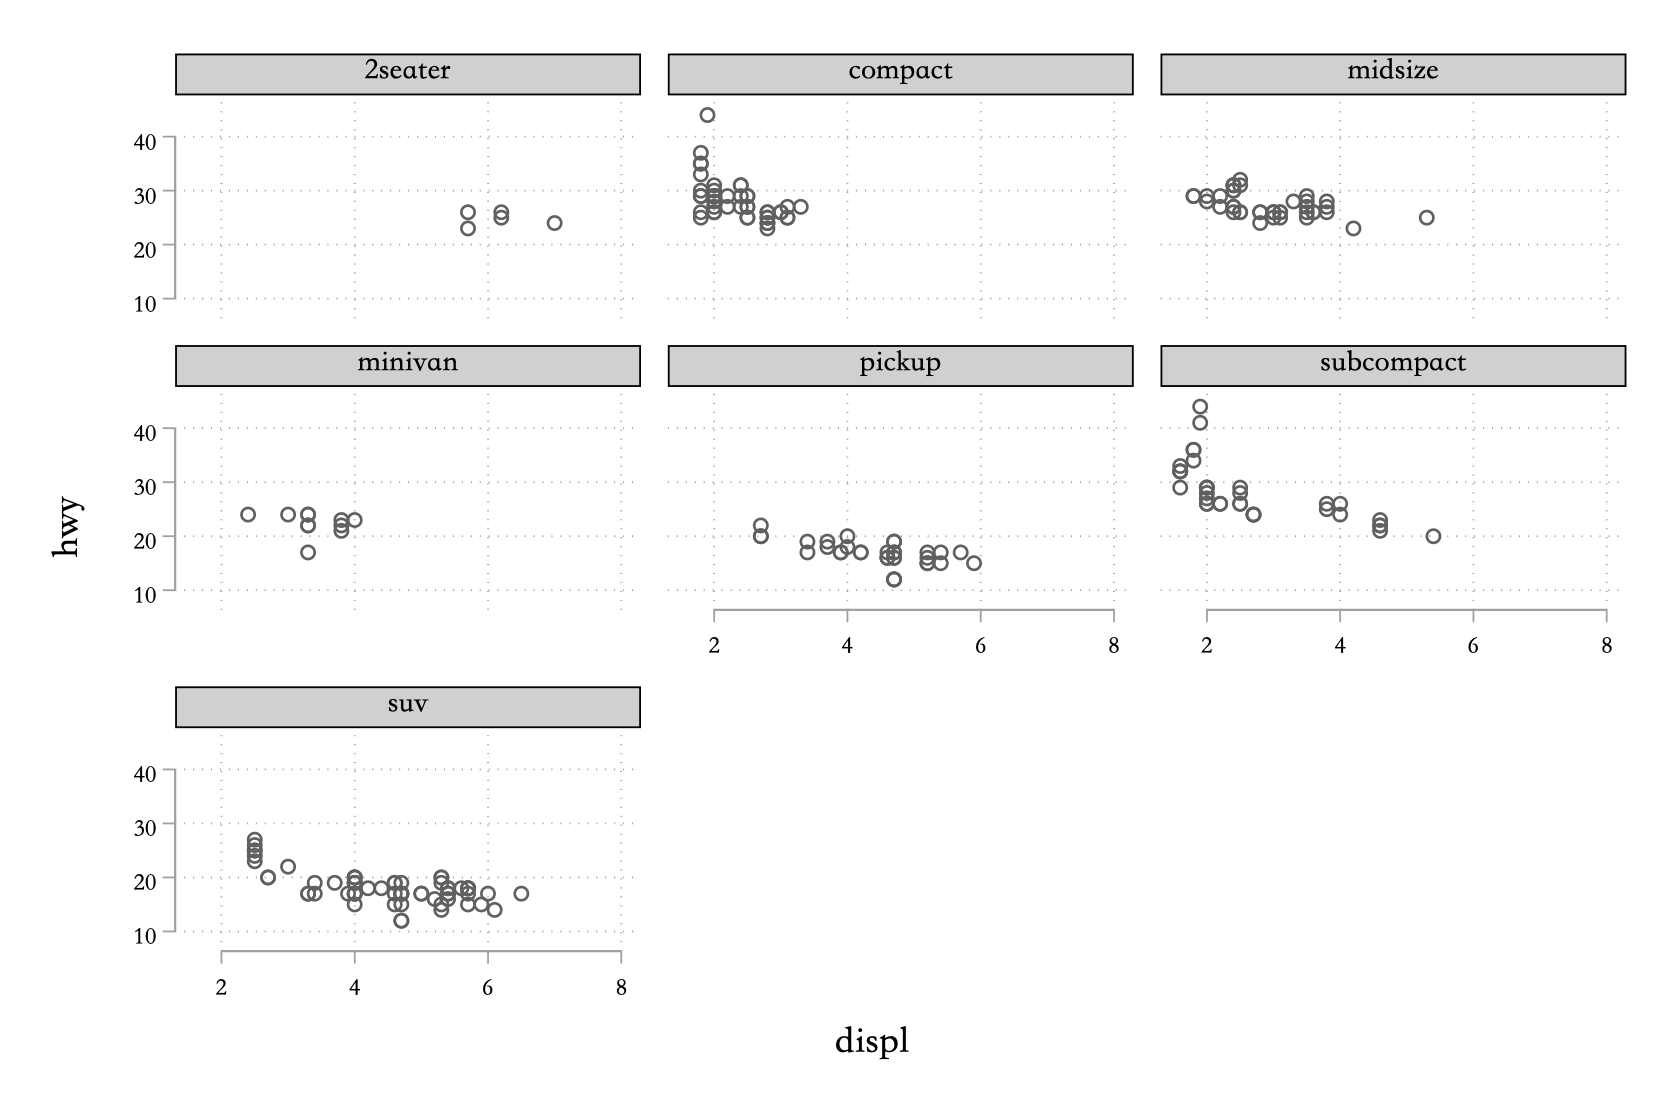
\includegraphics[width=1\textwidth]{assets/hwydisplbyclass3.png}
  \caption{不同型号汽车排量与燃油效率的关系}
  \label{fig:hwydisplbyclass3}
\end{figure}

\section{几何对象}

\begin{problem}
  观察图 \ref{fig:lpolychwydisp} 中的两个图层,什么相似的地方?

  \begin{lstlisting}
  tw ///
  sc hwy displ || ///
  lpolyci hwy disp
  \end{lstlisting}

  \begin{figure}[htbp]
    \centering
    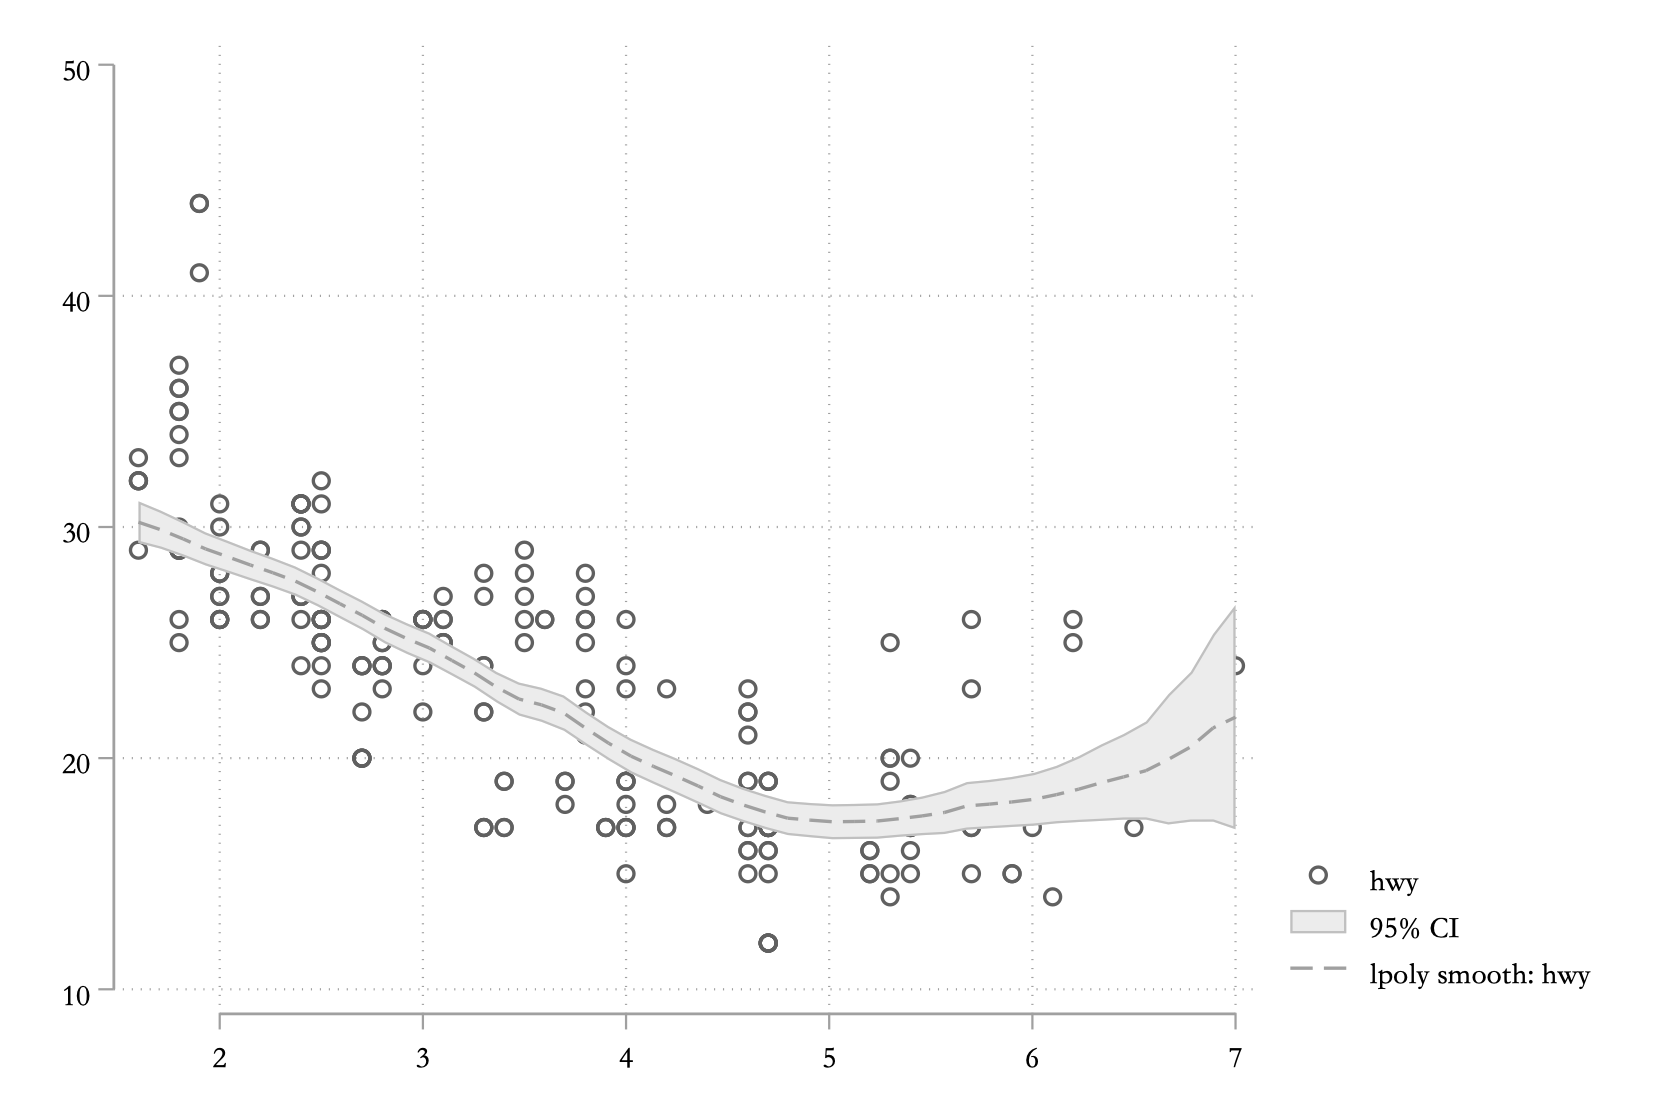
\includegraphics[width=\textwidth]{assets/lpolychwydisp.png}
    \caption{汽车排量与燃油效率的关系散点图与多项式拟合}
    \label{fig:lpolychwydisp}
  \end{figure}
\end{problem}

可以看出两个图层有着相同的x和y变量,也正是因此我们才能把这两个图层叠加在一起。但是一个是用散点表示两者的关系,一个是用多项式拟合线表示两者的关系,也就是说,两个图层使用了不同的几何对象。

人们经常会根据实际需要使用不同的几何对象表示数据,例如展示数据分布常使用直方图、箱线图,展示走势常使用线图等等。

图 \ref{fig:lpolycibydrv} 展示了针对不同的 drv 值绘制不同的曲线拟合:

\begin{lstlisting}
tw ///
lpolyci hwy displ if drv == "4", lp(solid) || ///
lpolyci hwy displ if drv == "f", lp(dash) || ///
lpolyci hwy displ if drv == "r", lp(shortdash) ||, ///
leg(order(2 "4" 4 "f" 6 "r") title(drv))
\end{lstlisting}

\begin{figure}[htbp]
  \centering
  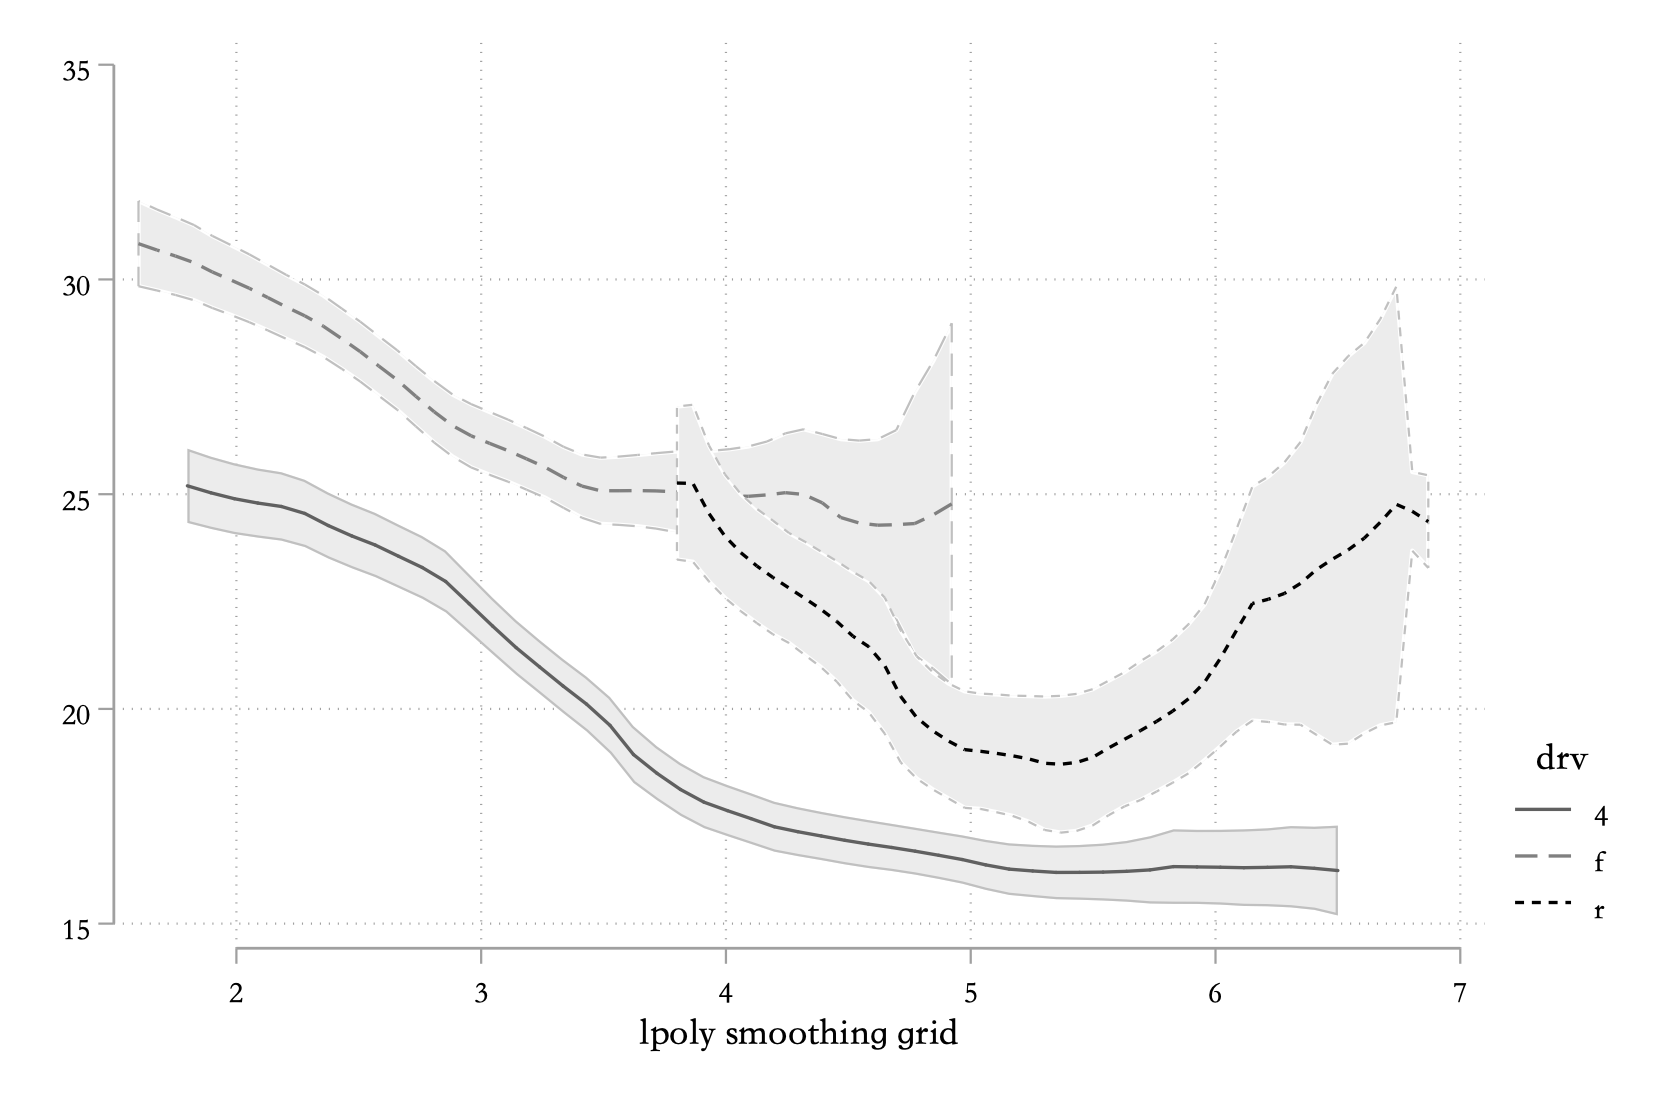
\includegraphics[width=\textwidth]{assets/lpolycibydrv.png}
  \caption{不同 drv 的汽车排量与燃油效率的关系}
  \label{fig:lpolycibydrv}
\end{figure}

这里需要补充的是,Stata中的线型有以下几种,如图 \ref{fig:linepalette}:

\begin{lstlisting}
palette linepalette
\end{lstlisting}

\begin{figure}[htbp]
  \centering 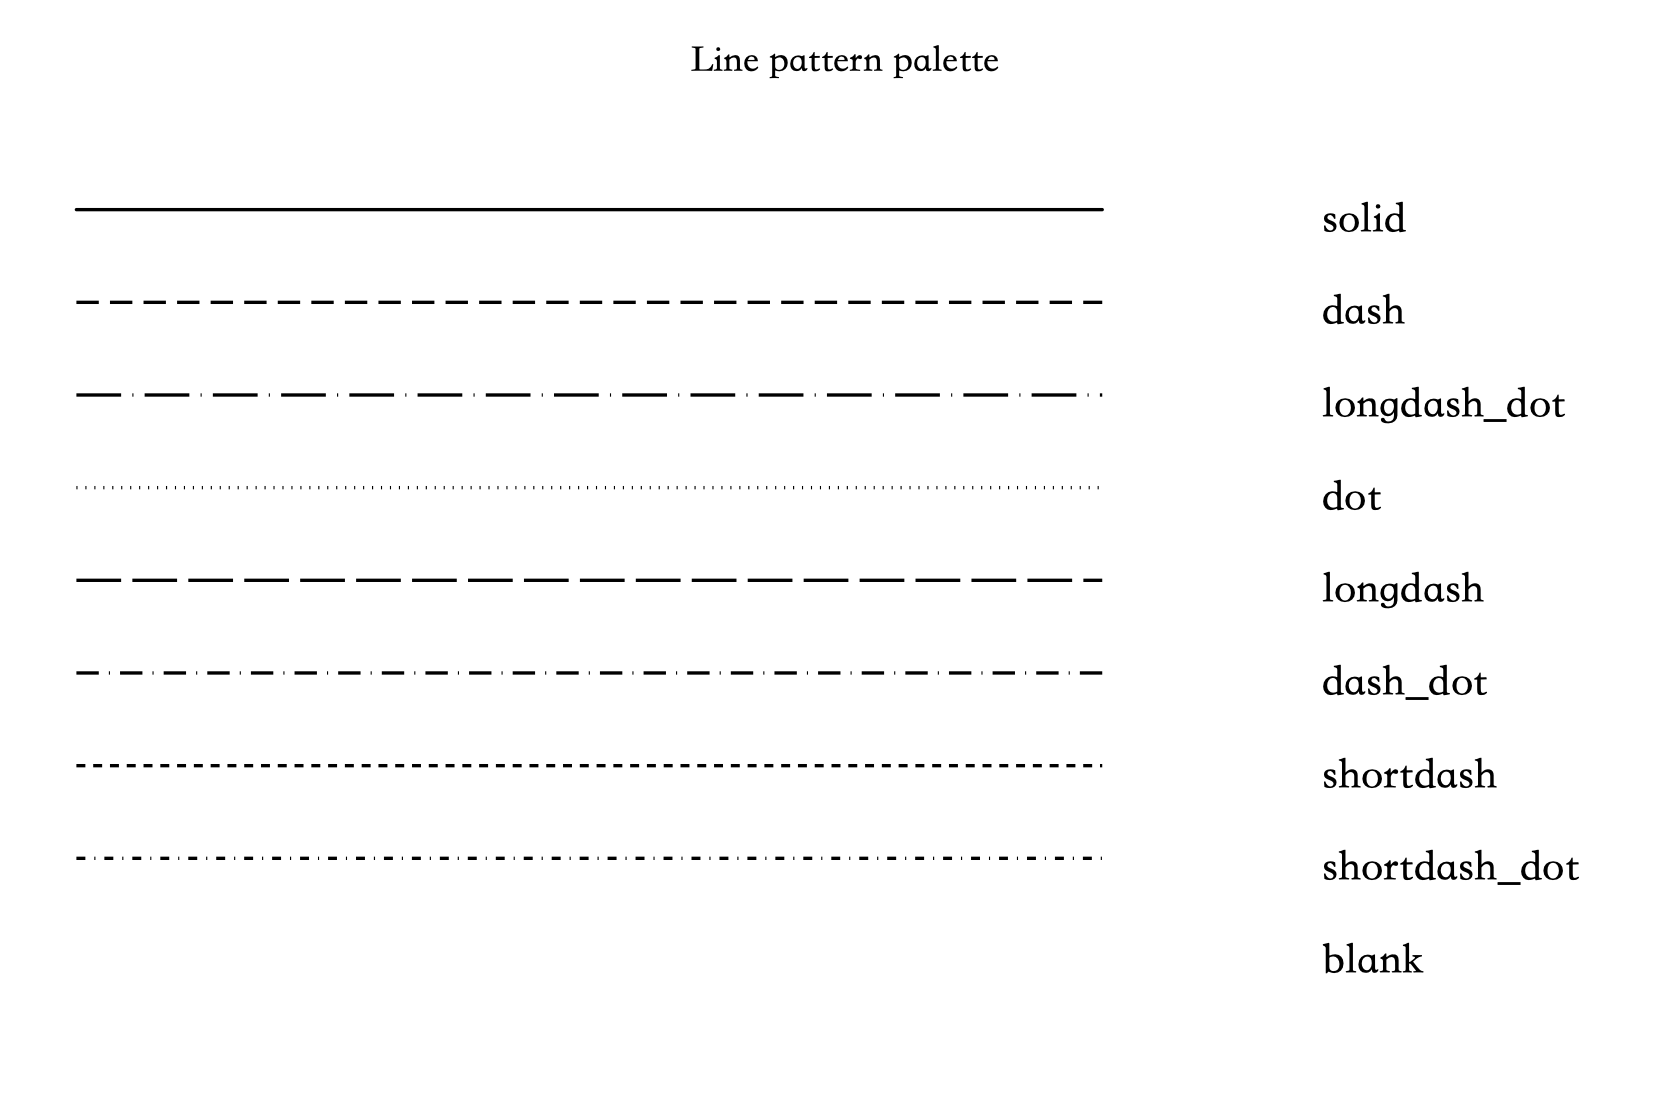
\includegraphics[width=\textwidth]{assets/linepalette.png}
  \caption{Stata 中的线型}\label{fig:linepalette}
\end{figure}

为了更容易区分,我们再对不同的图层使用不同的颜色,如图 \ref{fig:lpolycibydrv2}:

\begin{lstlisting}
colorscheme 3, palette("Set2")
return list
tw ///
lpolyci hwy displ if drv == "4", lc("`r(color1)'") || ///
lpolyci hwy displ if drv == "f", lc("`r(color2)'") || ///
lpolyci hwy displ if drv == "r", lc("`r(color3)'") || ///
sc hwy displ if drv == "4", mc("`r(color1)'") || ///
sc hwy displ if drv == "f", mc("`r(color2)'") || ///
sc hwy displ if drv == "r", mc("`r(color3)'") ||, ///
leg(order(2 "4" 4 "f" 6 "r") title(drv))
\end{lstlisting}

\begin{figure}[htbp]
  \centering 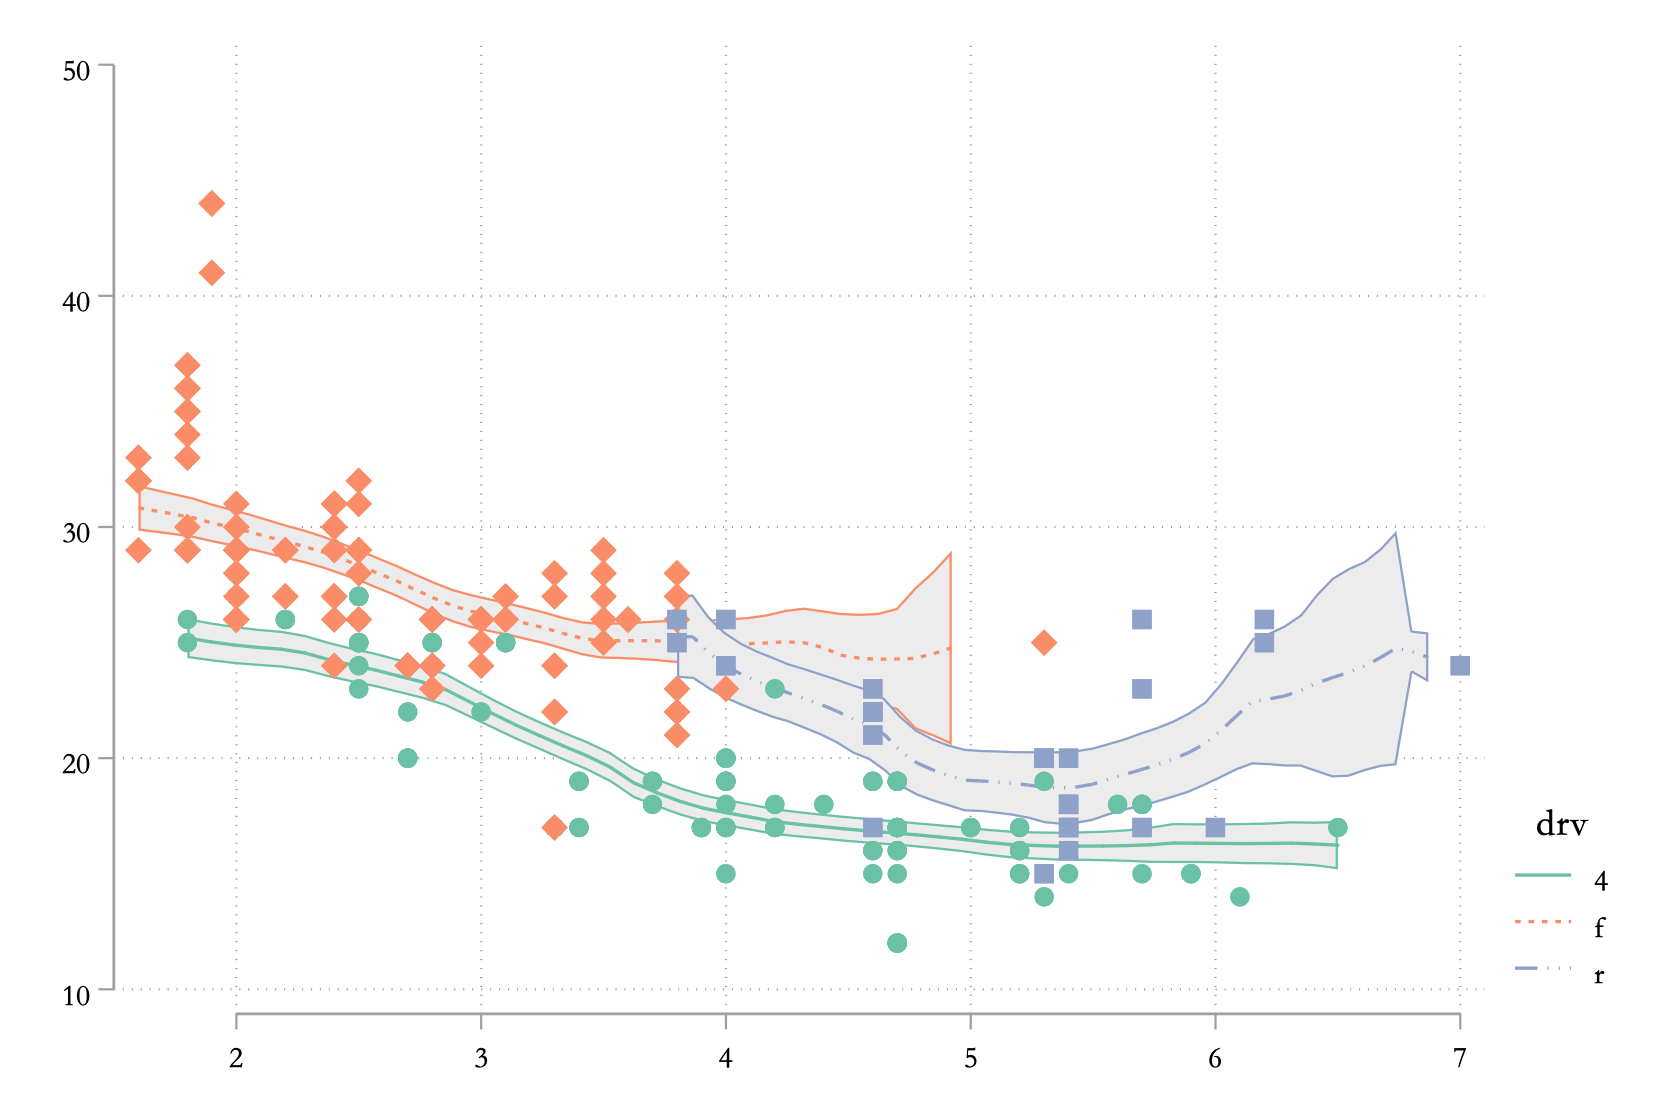
\includegraphics[width=\textwidth]{assets/lpolycibydrv2.png}
  \caption{不同 drv 的汽车排量与燃油效率的关系}
  \label{fig:lpolycibydrv2}
\end{figure}

Stata 的绘图功能是比较强大的,事实上我觉得如果一个绘图系统能够绘制不同颜色的点、线和区域,那么它就能够绘制任何图,而绘图的难易程度取决于绘图函数的设计。

图 \ref{fig:lpolycihwydispl} 展示了不同 class 的汽车排量与燃油效率的关系:

\begin{lstlisting}
colorscheme 8, palette(Set2)
tw ///
sc hwy displ if class == "2seater", mc("`r(color1)'") ms(o) || ///
sc hwy displ if class == "compact", mc("`r(color2)'") ms(o) || ///
sc hwy displ if class == "midsize", mc("`r(color3)'") ms(o) || ///
sc hwy displ if class == "minivan", mc("`r(color4)'") ms(o) || ///
sc hwy displ if class == "pickup", mc("`r(color5)'") ms(o) || ///
sc hwy displ if class == "subcompact", mc("`r(color6)'") ms(o) || ///
sc hwy displ if class == "suv", mc("`r(color7)'") ms(o) || ///
lpolyci hwy displ, lc("`r(color8)'") ||, ///
leg(order(1 "2seater" ///
          2 "compact" ///
          3 "midsize" ///
          4 "minivan" ///
          5 "pickup" ///
          6 "subcompact" ///
          7 "suv") title(class))
\end{lstlisting}

\begin{figure}[htbp]
  \centering
  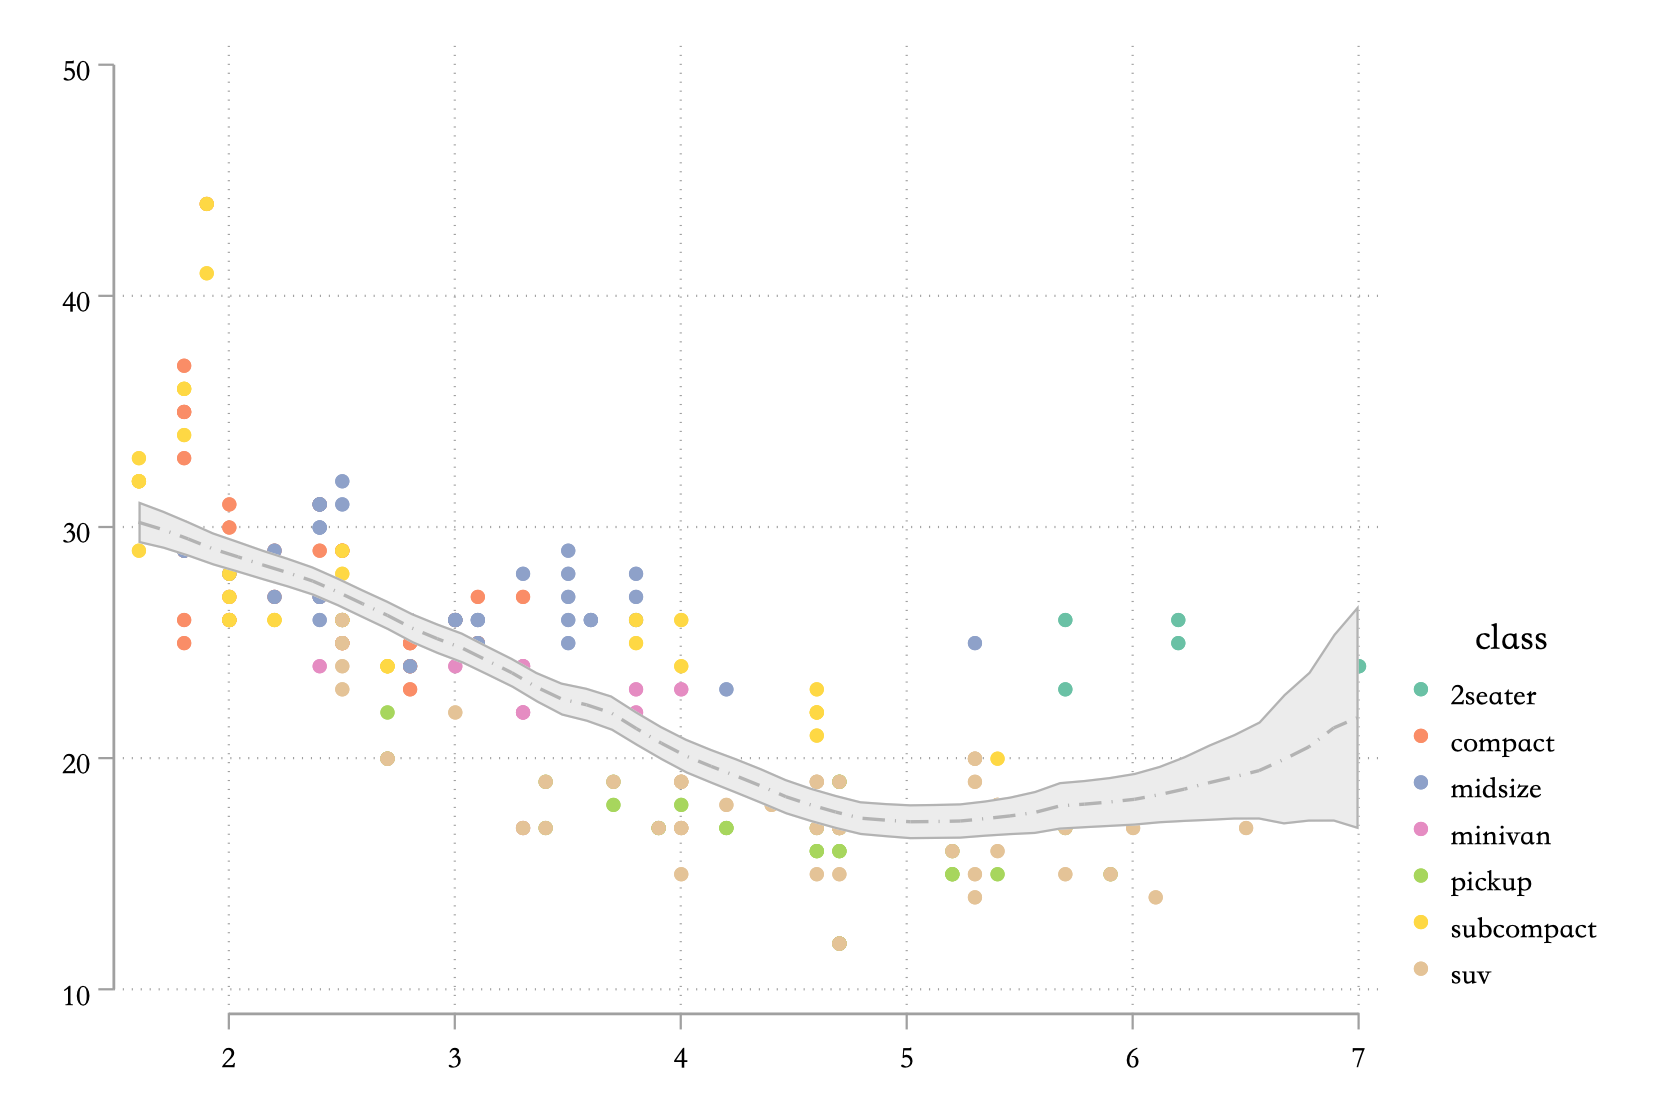
\includegraphics[width=\textwidth]{assets/lpolycihwydispl.png}
  \caption{不同 class 的汽车排量与燃油效率的关系}\label{fig:lpolycihwydispl}
\end{figure}

当然也可以对 class 的一个子集进行多项式拟合,如图 \ref{fig:lpolycihwydispl2}:

\begin{lstlisting}
colorscheme 8, palette(Set2)
tw ///
sc hwy displ if class == "2seater", mc("`r(color1)'") ms(o) || ///
sc hwy displ if class == "compact", mc("`r(color2)'") ms(o) || ///
sc hwy displ if class == "midsize", mc("`r(color3)'") ms(o) || ///
sc hwy displ if class == "minivan", mc("`r(color4)'") ms(o) || ///
sc hwy displ if class == "pickup", mc("`r(color5)'") ms(o) || ///
sc hwy displ if class == "subcompact", mc("`r(color6)'") ms(o) || ///
sc hwy displ if class == "suv", mc("`r(color7)'") ms(o) || ///
lpolyci hwy displ if class == "subcompact", lc("`r(color8)'") ||, ///
leg(order(1 "2seater" ///
          2 "compact" ///
          3 "midsize" ///
          4 "minivan" ///
          5 "pickup" ///
          6 "subcompact" ///
          7 "suv") title(class))
\end{lstlisting}

\begin{figure}[htbp]
  \centering
  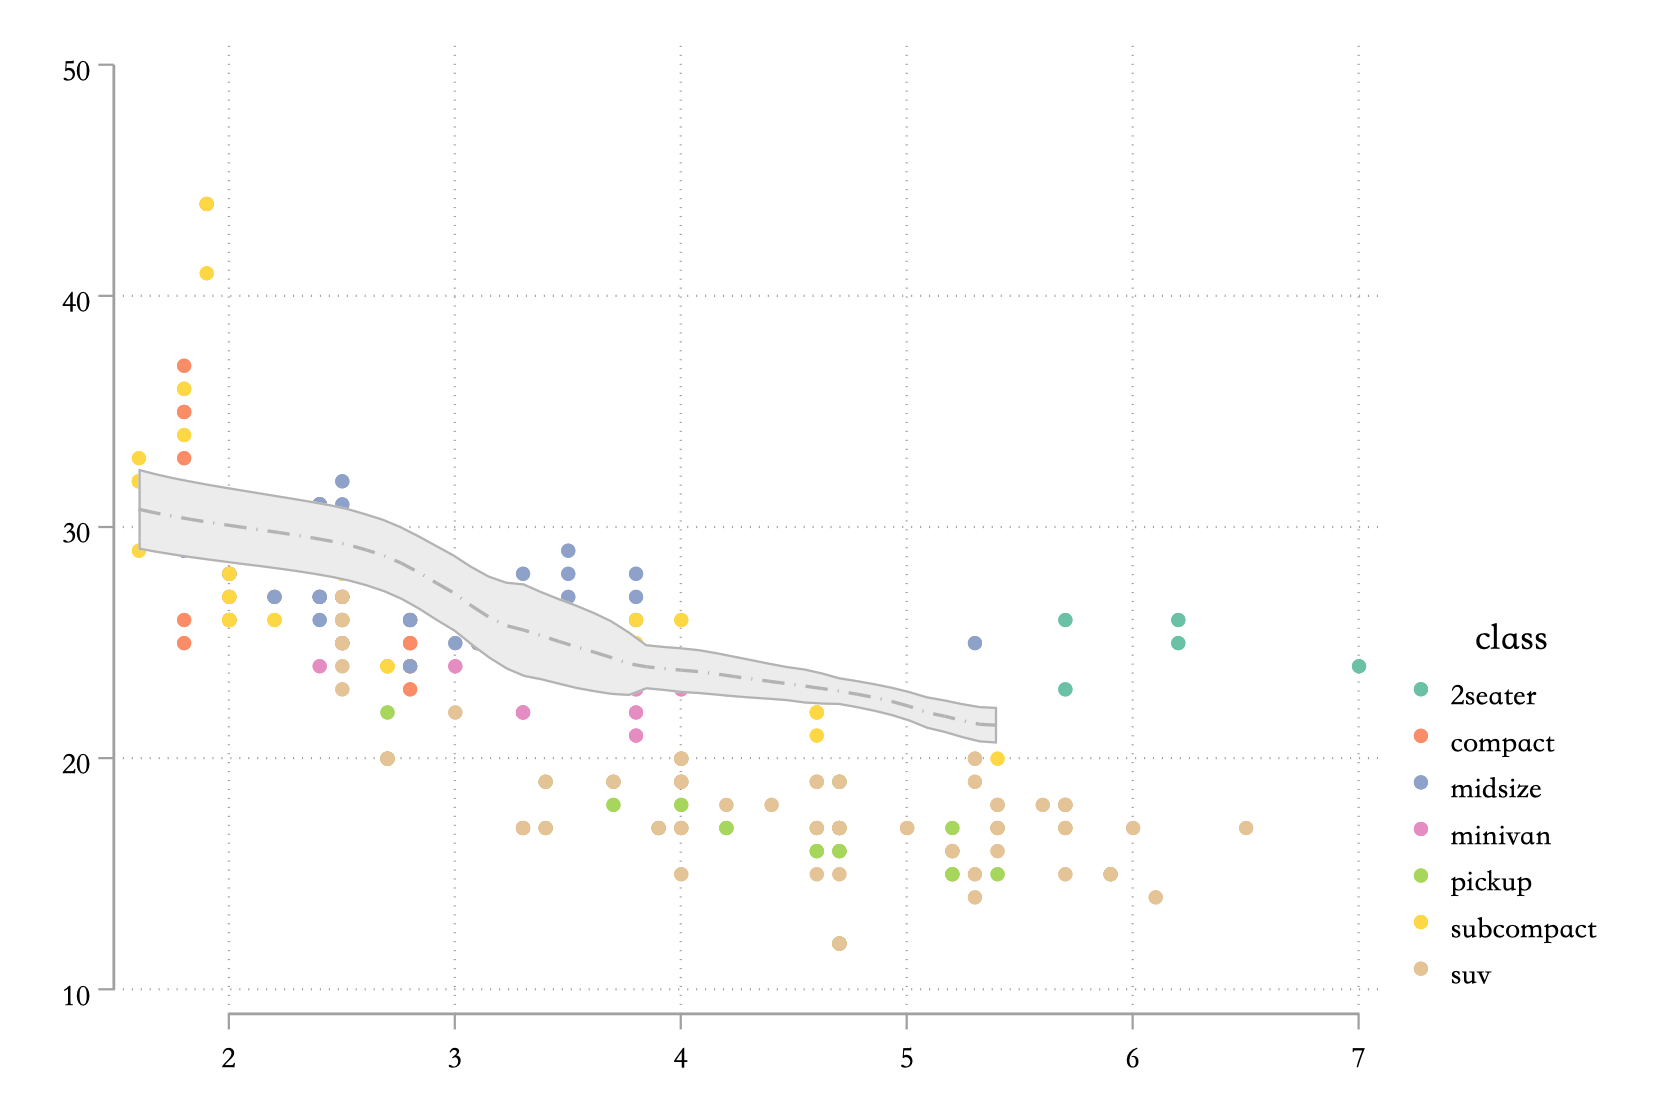
\includegraphics[width=\textwidth]{assets/lpolycihwydispl2.png}
  \caption{不同 class 的汽车排量与燃油效率的关系}
  \label{fig:lpolycihwydispl2}
\end{figure}

\section{统计变换}

Stata 绘制直方图的命令是 \texttt{histogram} ,简写为 \texttt{hist},如图 \ref{fig:histcut}:

\begin{lstlisting}
sysuse diamonds, clear
hist cut, barwidth(0.8) xlab(, val) freq
\end{lstlisting}

\begin{figure}[htbp]
  \centering
  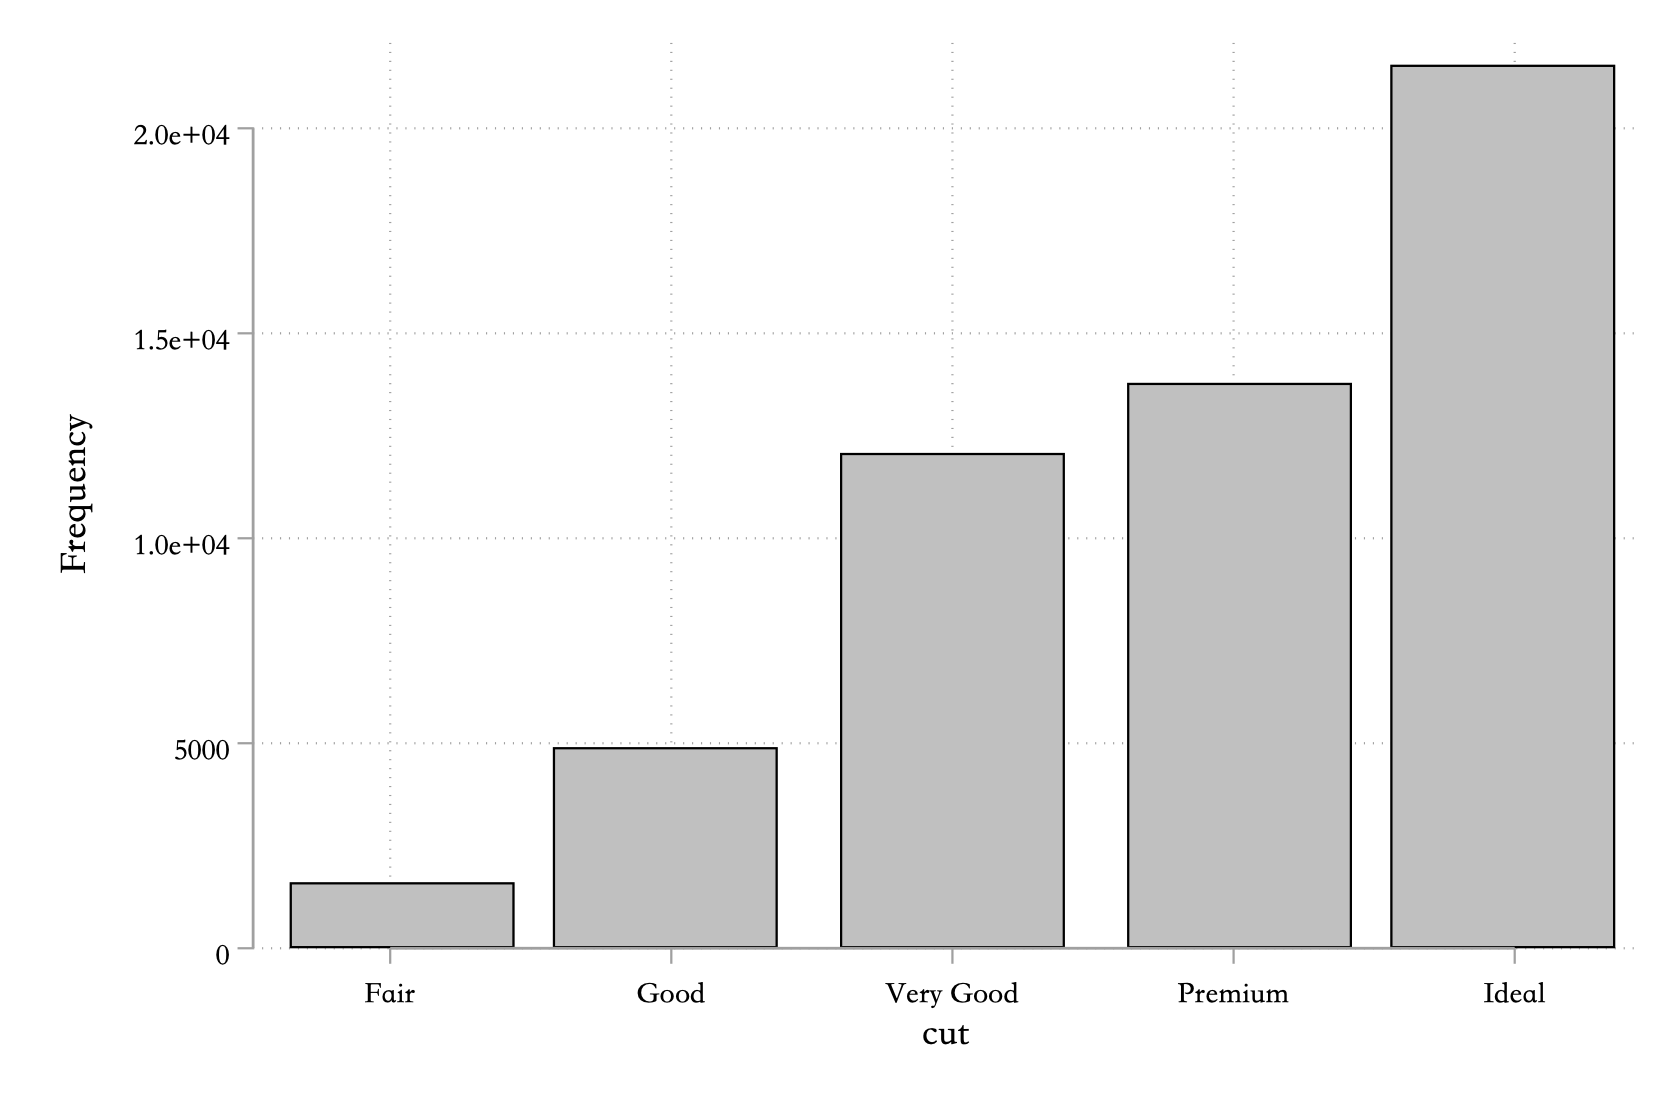
\includegraphics[width=0.8\textwidth]{assets/histcut.png}
  \caption{钻石切工分布直方图}\label{fig:histcut}
\end{figure}

我们可以注意到,图 \ref{fig:histcut} 中的横轴是 cut 变量,纵轴是 cut 变量各个取值的分布,而我们主要到数据集中是没有这个变量的,显然这个变量是 hist 命令计算过程中生成的,下面的语句展示了如何对 cut 变量的各个取值进行计数然后绘制直方图,如图 \ref{fig:barcut}:

\begin{lstlisting}
contract cut
tw bar _freq cut, barwidth(0.8) xlab(, val)
\end{lstlisting}

\begin{figure}[htbp]
  \centering
  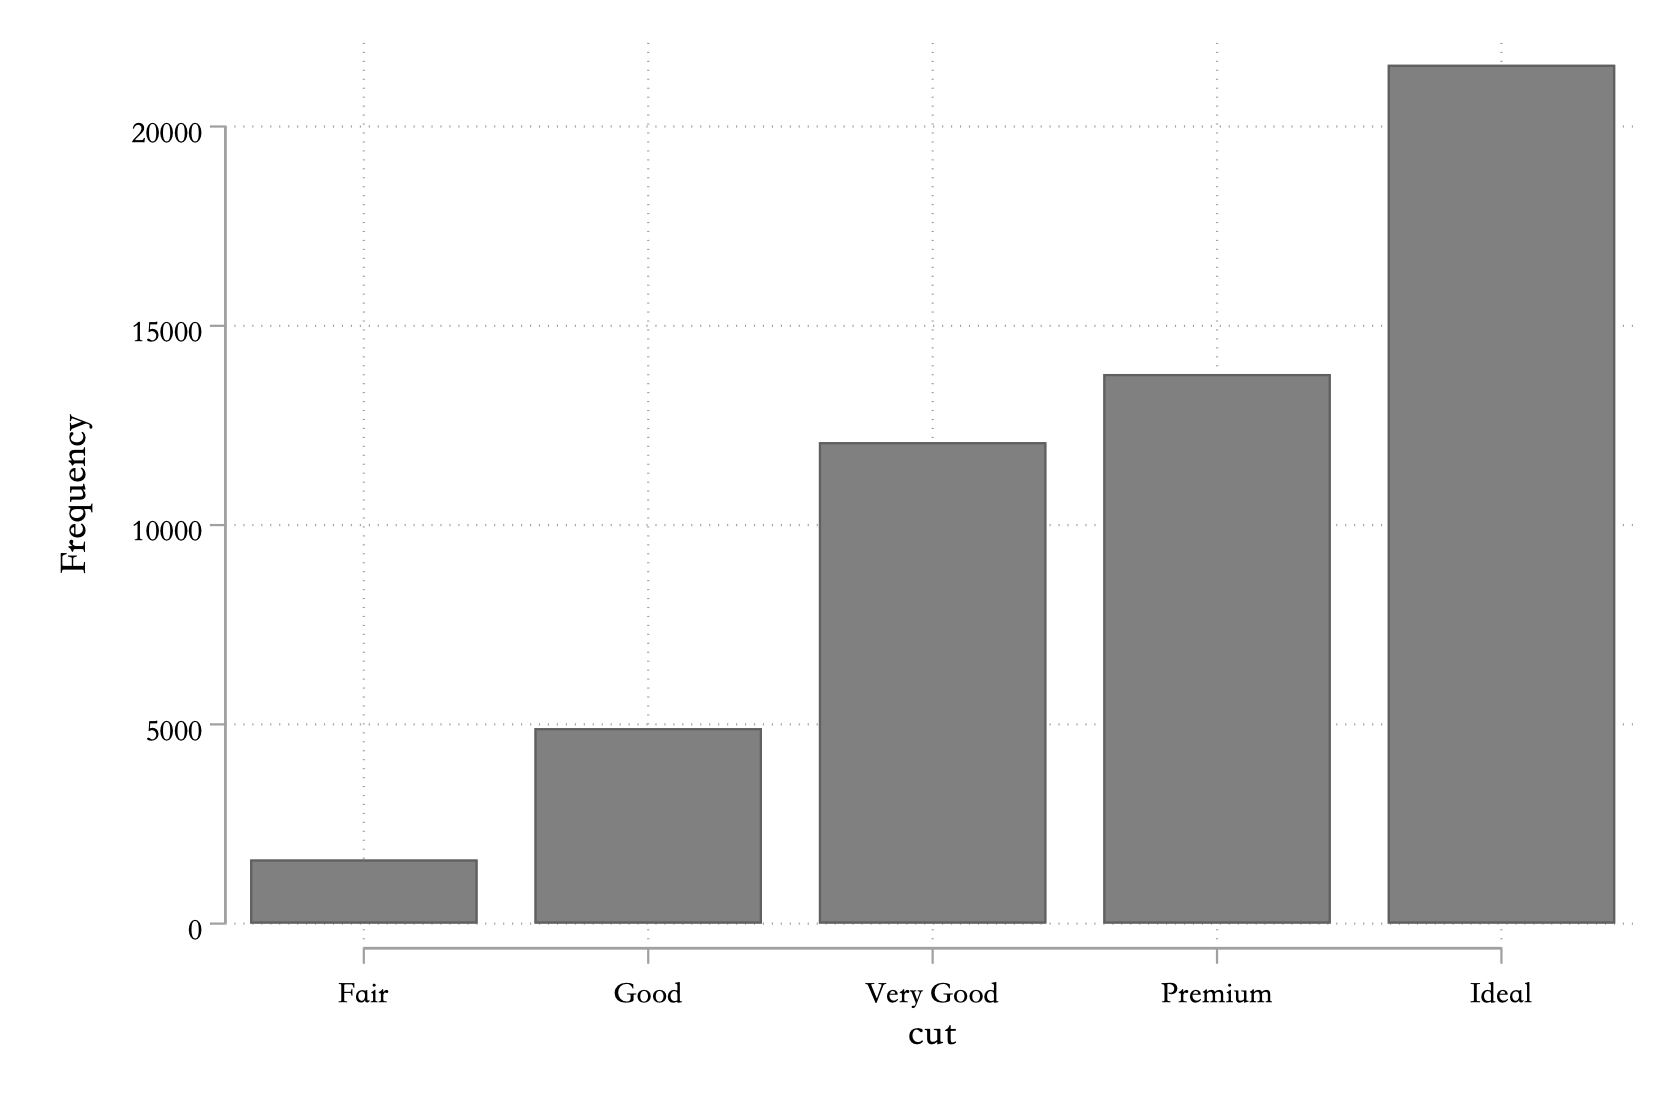
\includegraphics[width=\textwidth]{assets/barcut.png}
  \caption{钻石切工分布直方图}\label{fig:barcut}
\end{figure}

contract 命令能够快速的对变量进行计数,详细用法可以参考其帮助文档(help contract)或者我的博客文章: \href{https://www.czxa.top/posts/1170/\#contract\%E5\%91\%BD\%E4\%BB\%A4}{Stata旧笔记整理(八)\#contract命令}。

contract 命令运行之后会生成一个新的数据集,如表 \ref{tab:cut}:

\begin{table}[htbp]
\caption{\label{tab:cut}contract cut 的结果}
\centering
\begin{tabular}{lr}
\toprule
cut & \_freq\\
\midrule
Fair & 1610\\
Good & 4906\\
Very Good & 12082\\
Premium & 13791\\
Ideal & 21551\\
\bottomrule
\end{tabular}
\end{table}

通过这个过程你就会发现所谓的 \textcolor{third3}{统计变换} 不过就是把一系列的计算过程封装在命令中,并不难懂。

\texttt{hist} 命令的纵轴也可以为频率(Density),去掉 freq 选项即可,如图 \ref{fig:histcut2}:

\begin{lstlisting}
sysuse diamonds, clear
hist cut, barwidth(0.8) xlab(, val)
\end{lstlisting}

\begin{figure}[htbp]
  \centering 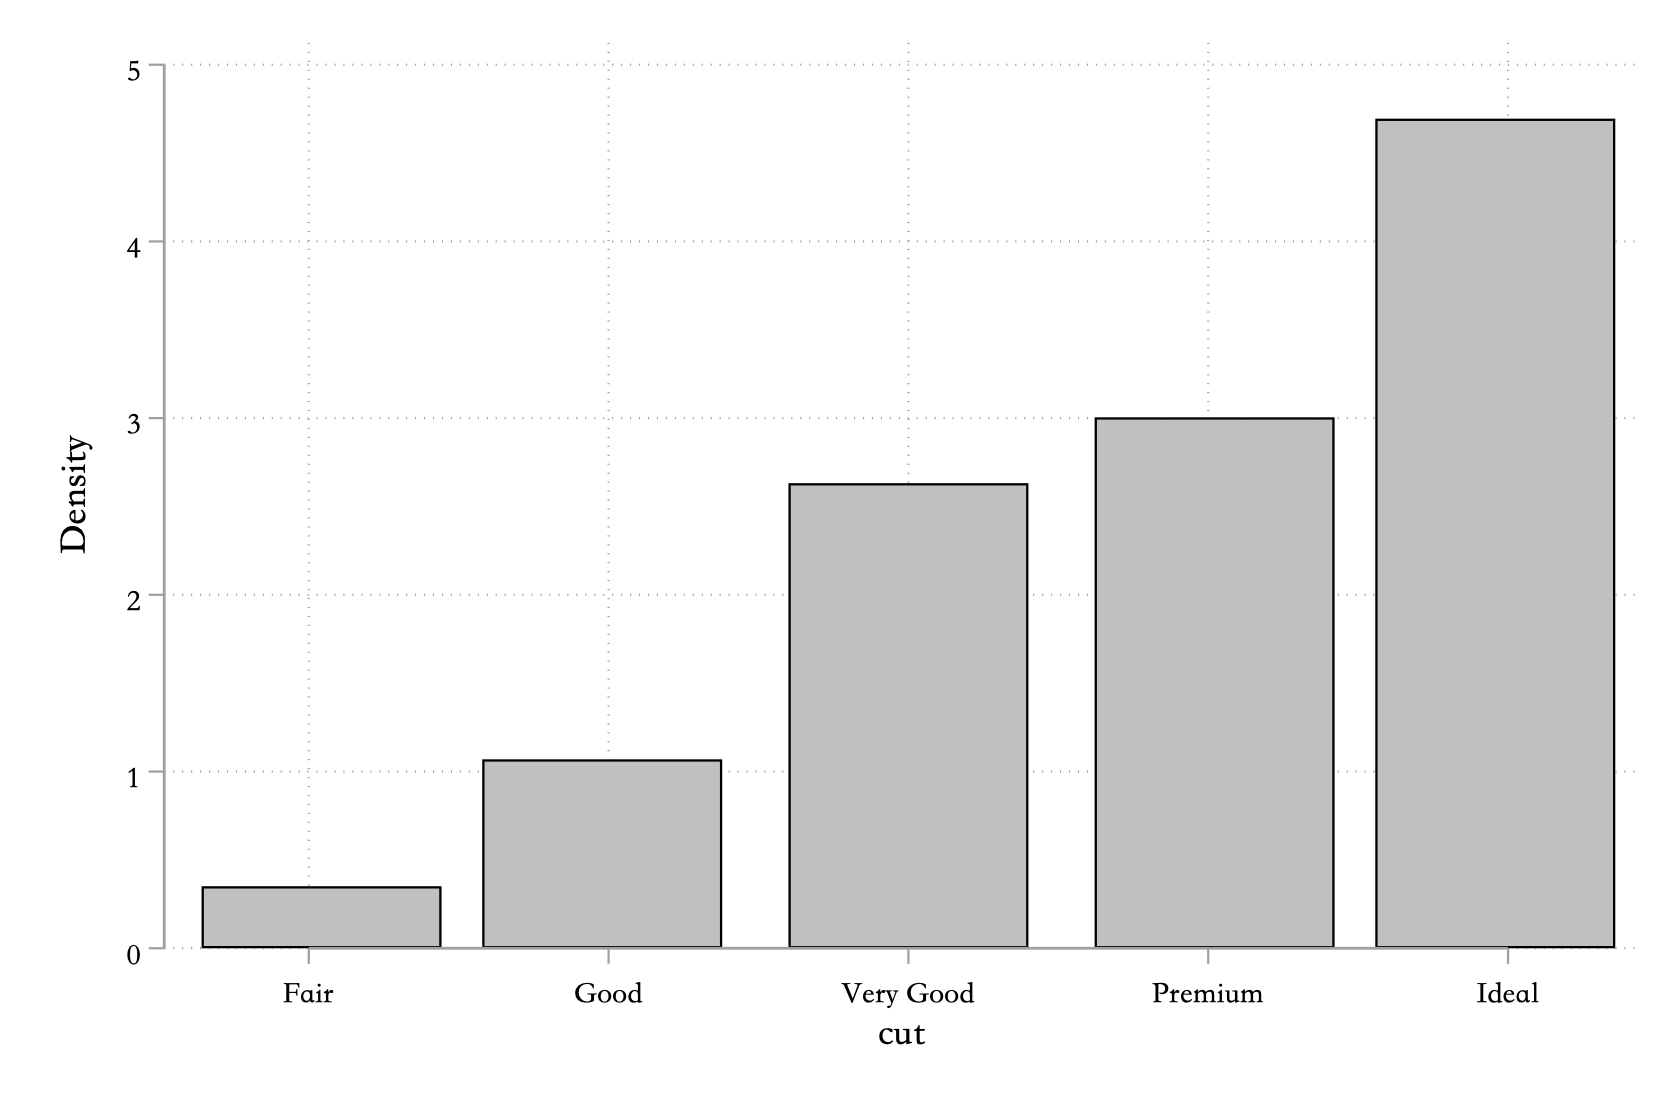
\includegraphics[width=\textwidth]{assets/histcut2.png}
  \caption{钻石切工分布直方图}\label{fig:histcut2}
\end{figure}

统计变换经常是件苦力活,因为很多时候我们需要先计算我们需要进行的统计变换,然后再把变换后的结果整理好读入Stata再绘图,\lstinline{collapse} 是一个非常好用的命令,可以帮我们简化这个过程,例如我想展示不同cut值depth变量的范围和中位数:

\begin{lstlisting}
sysuse diamonds, clear
collapse    (min) depthmin = depth ///
            (median) depthmedian = depth ///
            (max) depthmax = depth, by(cut)
\end{lstlisting}

这个时候得到的结果见表 \ref{tab:depthmmm}:

\begin{table}[htbp]
\caption{\label{tab:depthmmm}collapse depth 的结果}
\centering
\begin{tabular}{lrrr}
\toprule
cut & depthmin & depthmedian & depthmax\\
\midrule
Fair & 43.0 & 65.0 & 79.0\\
Good & 54.3 & 63.4 & 67.0\\
Very Good & 56.8 & 62.1 & 64.9\\
Premium & 58.0 & 61.4 & 63.0\\
Ideal & 43.0 & 61.8 & 66.7\\
\bottomrule
\end{tabular}
\end{table}

然后我们再绘图,绘图结果见图 \ref{fig:depth3m}:

\begin{lstlisting}
tw ///
rspike depthmax depthmin cut || ///
sc depthmedian cut, xlab(, val) ms(O) mc(black) ||, ///
leg(off)
\end{lstlisting}

\begin{figure}[htbp]
  \centering 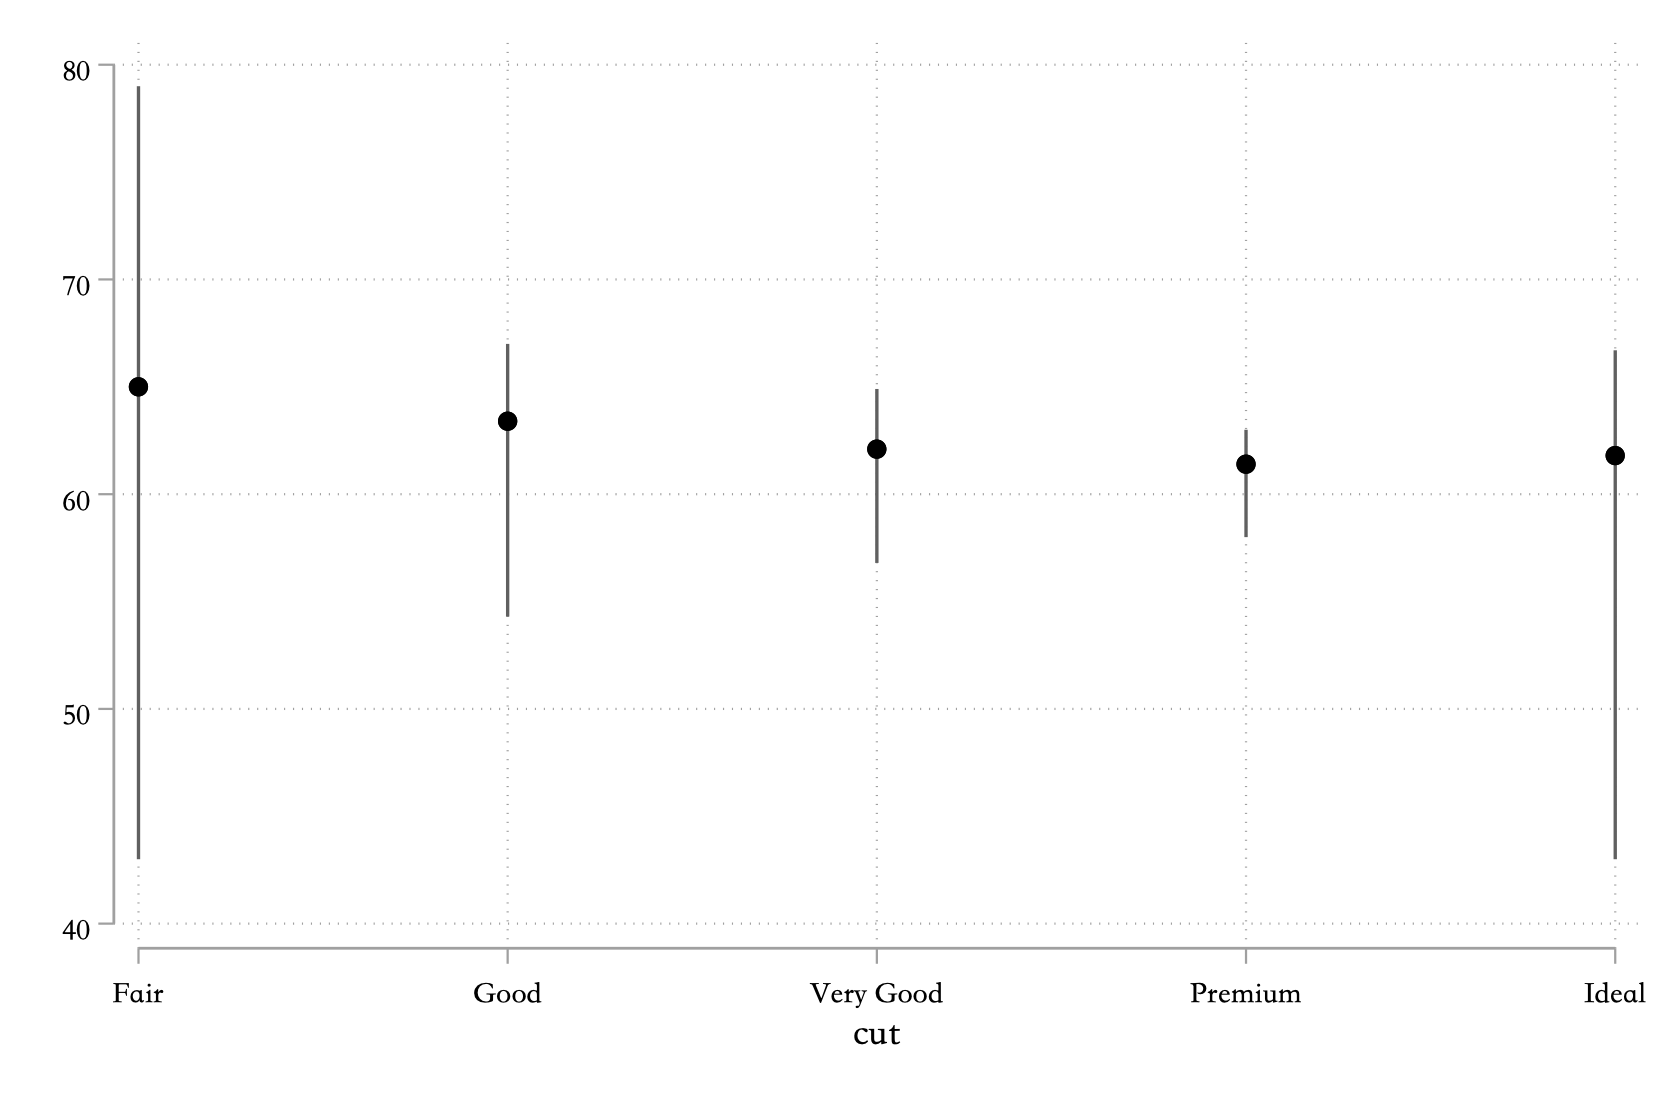
\includegraphics[width=\textwidth]{assets/depth3m.png}
  \caption{钻石深度的分布}
  \label{fig:depth3m}
\end{figure}

\section{位置调整}

通过不同的颜色设置,我们可以得到下面的图 \ref{fig:barcutmulticolor} 和图 \ref{fig:barcutmulticolor2}:

\begin{lstlisting}
sysuse diamonds, clear
contract cut
colorscheme 5, palette(Set2)
tw ///
bar _freq cut if cut == 1, fc("`r(color1)'") barwidth(0.8) || ///
bar _freq cut if cut == 2, fc("`r(color2)'") barwidth(0.8) || ///
bar _freq cut if cut == 3, fc("`r(color3)'") barwidth(0.8) || ///
bar _freq cut if cut == 4, fc("`r(color4)'") barwidth(0.8) || ///
bar _freq cut if cut == 5, fc("`r(color5)'") ///
barwidth(0.8) xlab(, val) leg(off)
\end{lstlisting}

\begin{figure}[htbp]
  \centering
  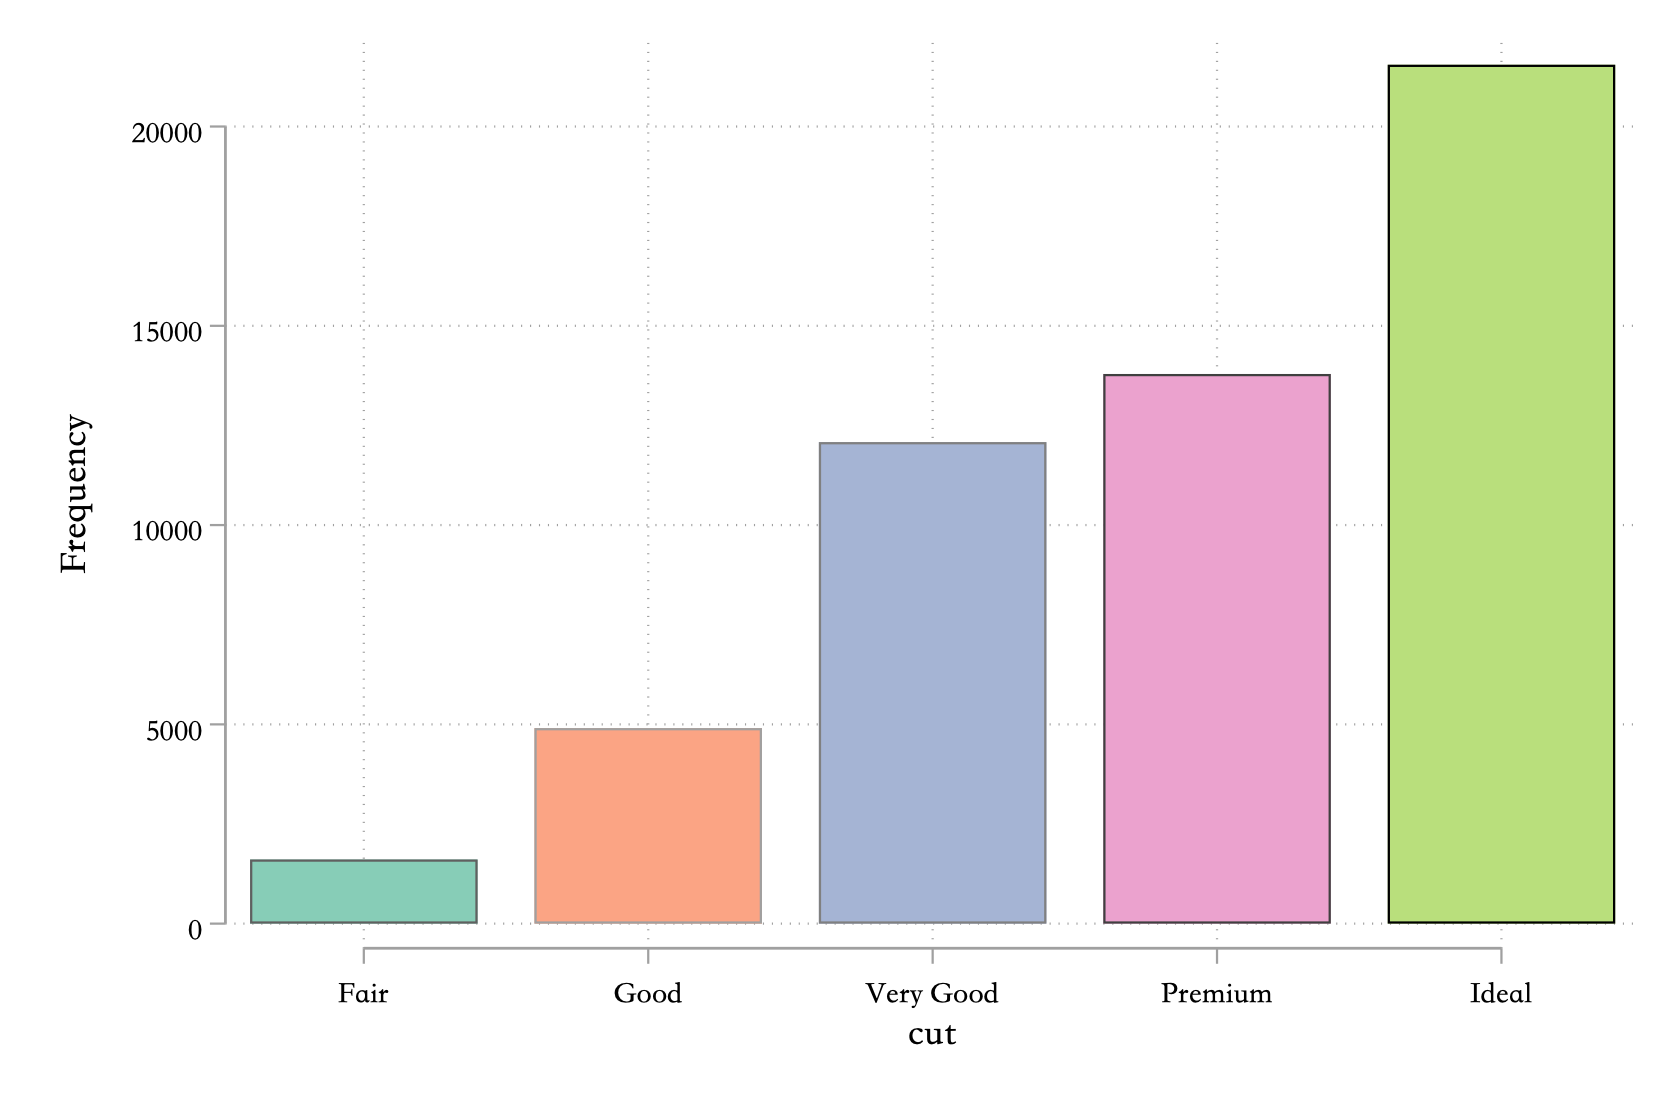
\includegraphics[width=\textwidth]{assets/barcutmulticolor.png}
  \caption{钻石切工的分布}\label{fig:barcutmulticolor}
\end{figure}

\begin{lstlisting}
sysuse diamonds, clear
contract cut
colorscheme 5, palette(Set1)
tw ///
bar _freq cut if cut == 1, lc("`r(color1)'") barwidth(0.8) || ///
bar _freq cut if cut == 2, lc("`r(color2)'") barwidth(0.8) || ///
bar _freq cut if cut == 3, lc("`r(color3)'") barwidth(0.8) || ///
bar _freq cut if cut == 4, lc("`r(color4)'") barwidth(0.8) || ///
bar _freq cut if cut == 5, lc("`r(color5)'") ///
barwidth(0.8) xlab(, val) leg(off)
\end{lstlisting}

\begin{figure}[htbp]
  \centering
  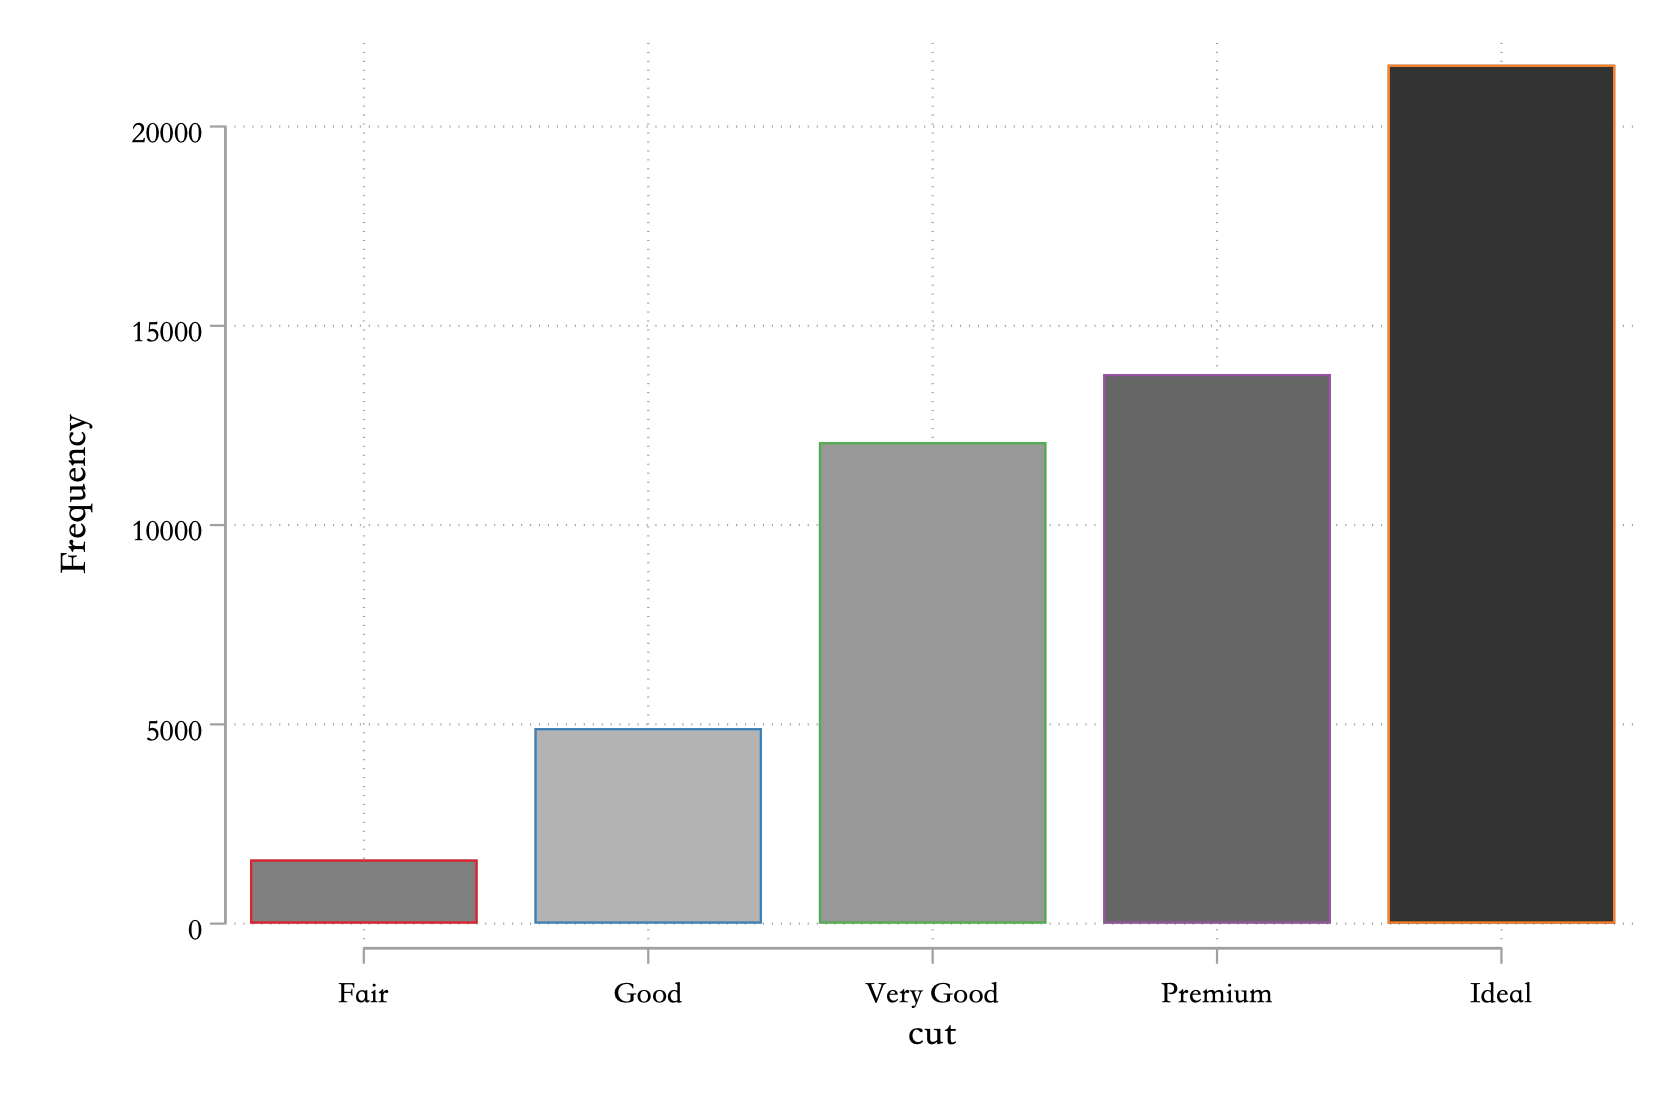
\includegraphics[width=\textwidth]{assets/barcutmulticolor2.png}
  \caption{钻石切工的分布}
  \label{fig:barcutmulticolor2}
\end{figure}

两幅图的区别就在于,第一幅图是使用 \texttt{fc()} 选项,这个选项控制对直方条的填充色,第二幅图使用的是 \texttt{lc()} 选项,这个选项控制直方条边缘的颜色。

实际上,上面两幅图关于颜色的设置都是没有什么实际意义的,只是让图看起来更加炫酷。但是有时候我们想知道例如``我们班的男生和女生生源地分布''这种问题的答案,这个时候使用颜色填充就有意义了,例如图 \ref{fig:stackcutclarity}钻石不同切工的克拉分布:

\begin{lstlisting}
sysuse diamonds, clear
colorscheme 8, palette(Paired)
gr bar, over(clarity) over(cut) ///
    stack asyvars yti(count) ///
    leg(ti(clarity)) ///
    bar(1, color("`r(color1)'")) ///
    bar(2, color("`r(color2)'")) ///
    bar(3, color("`r(color3)'")) ///
    bar(4, color("`r(color4)'")) ///
    bar(5, color("`r(color5)'")) ///
    bar(6, color("`r(color6)'")) ///
    bar(7, color("`r(color7)'")) ///
    bar(8, color("`r(color8)'"))
\end{lstlisting}

\begin{figure}[htbp]
  \centering
  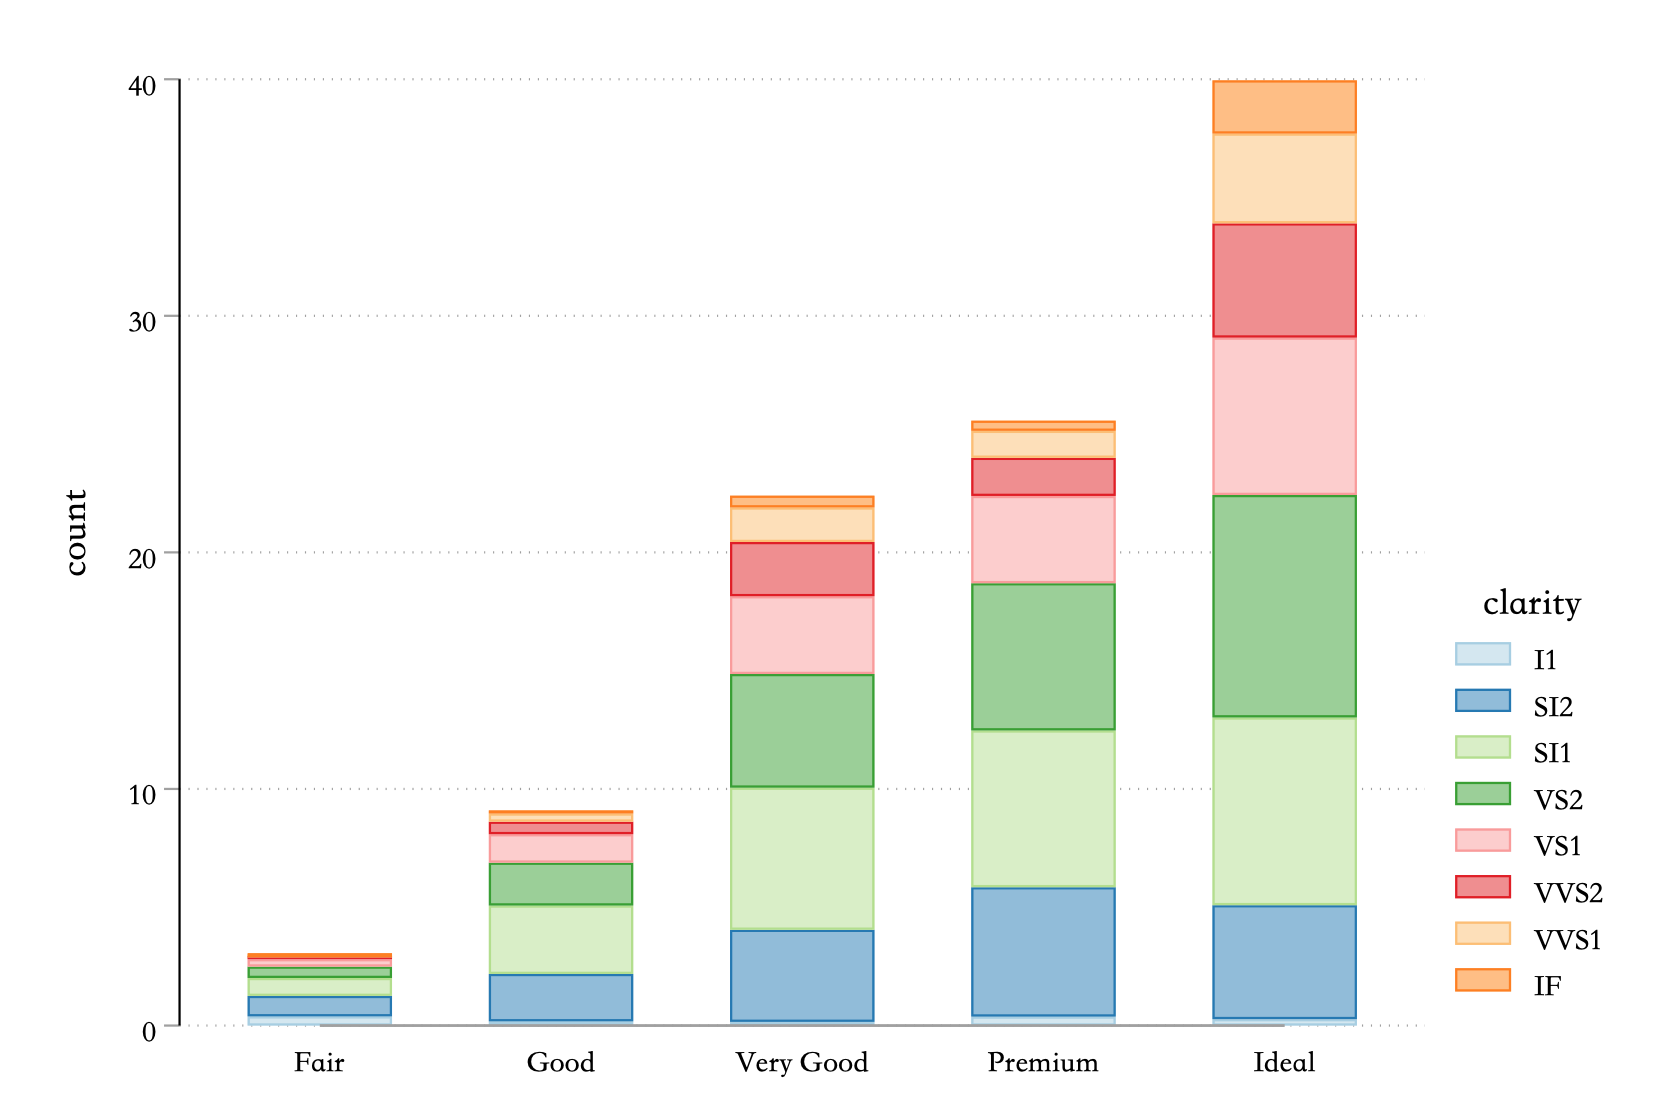
\includegraphics[width=\textwidth]{assets/stackcutclarity.png}
  \caption{钻石不同切工的克拉分布}\label{fig:stackcutclarity}
\end{figure}

有时候我们会绘制图 \ref{fig:histautoprice}:

\begin{lstlisting}
sysuse auto, clear
tw ///
hist price if for || ///
hist price if !for
\end{lstlisting}

\begin{figure}[htbp]
  \centering 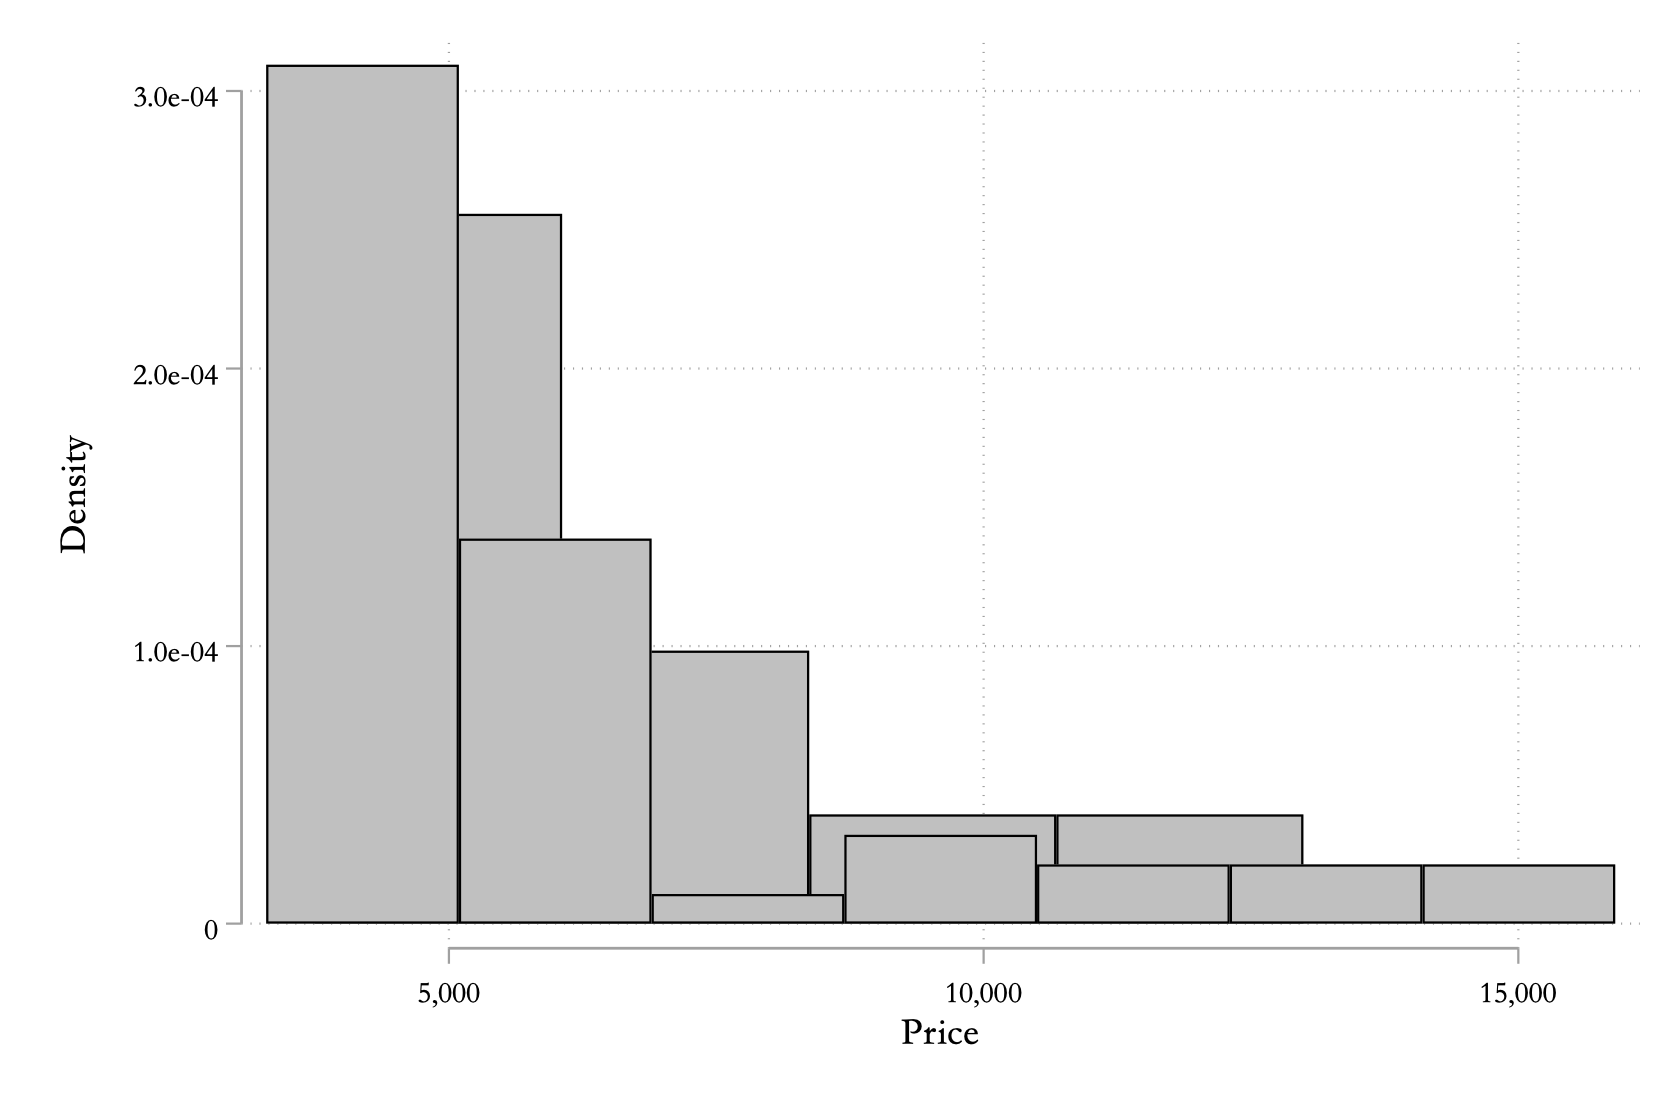
\includegraphics[width=0.8\textwidth]{assets/histautoprice.png}
  \caption{国产车和进口车的价格分布}\label{fig:histautoprice}
\end{figure}

这个图的问题就是相互重叠问题很严重,为此我们可以采取下面两种方法解决这个问题,第一种是将位于上层的图层设置为透明的,如图 \ref{fig:histautoprice2}:

\begin{lstlisting}
tw ///
hist price if for, fc(red) || ///
hist price if !for, fc(green%50) ///
    leg(order(1 "进口车" 2 "国产车"))
\end{lstlisting}

\begin{figure}[htbp]
  \centering
  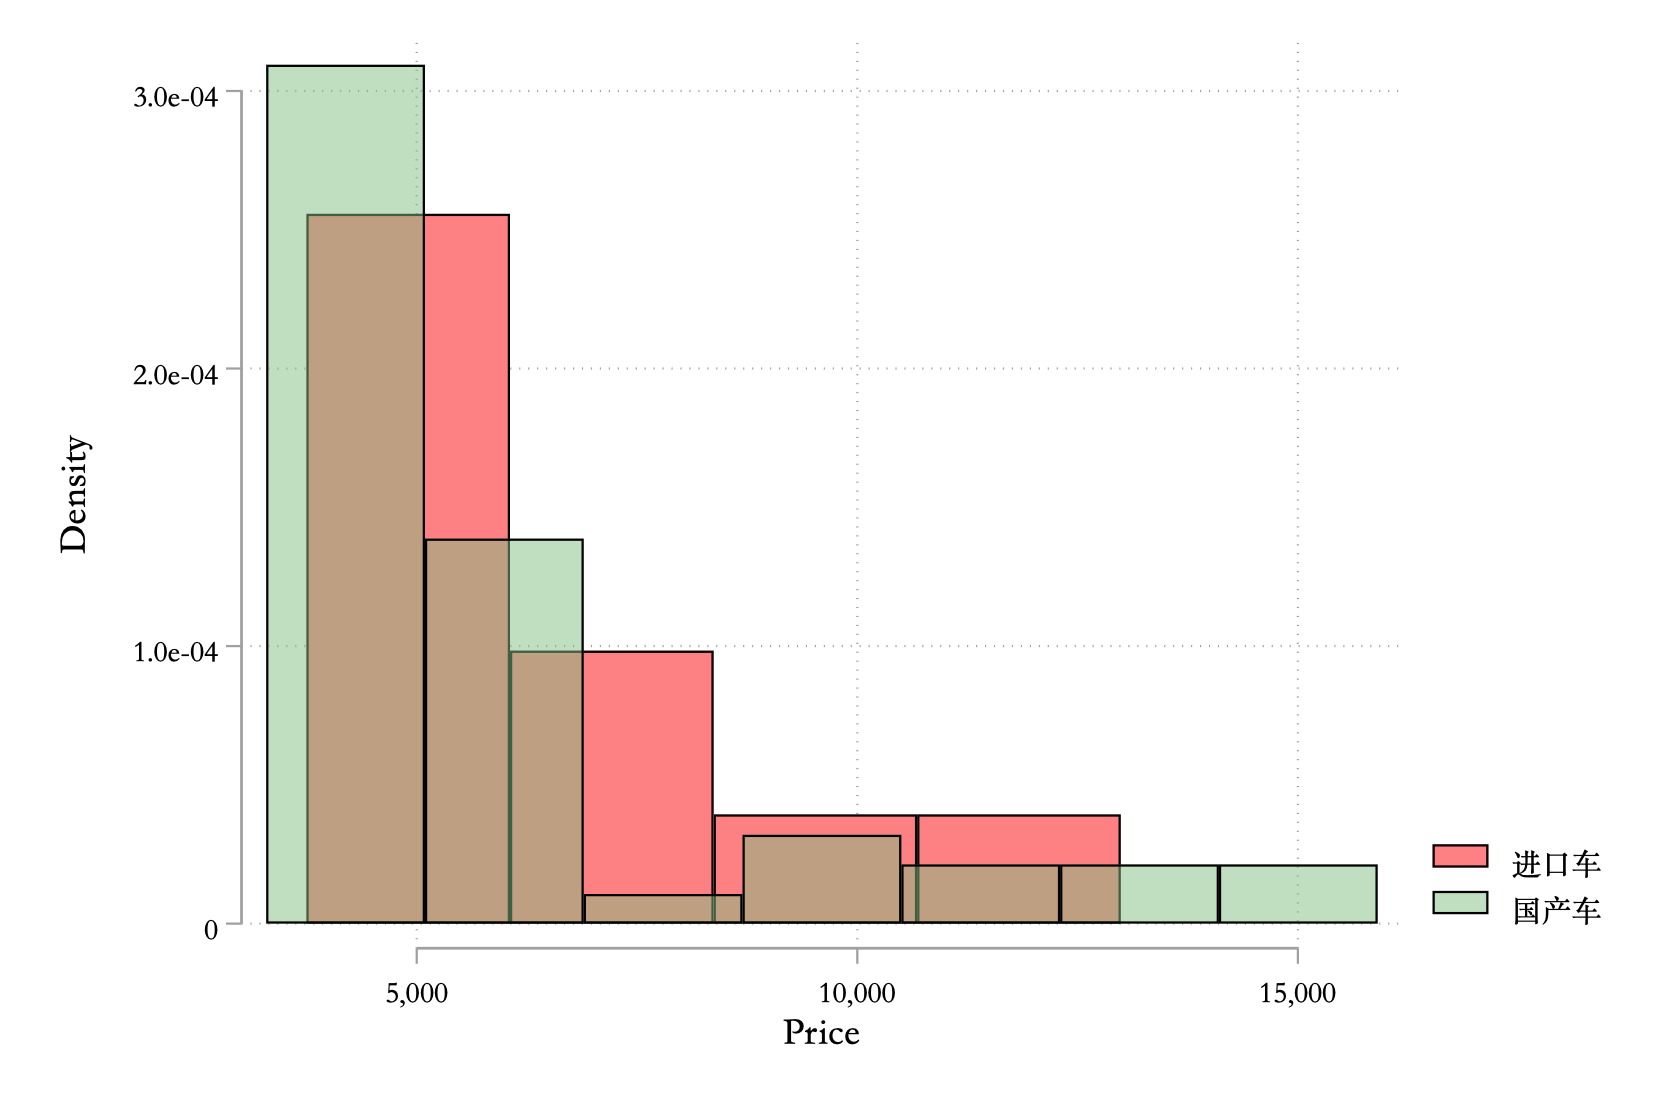
\includegraphics[width=\textwidth]{assets/histautoprice2.png}
  \caption{国产车和进口车的价格分布}\label{fig:histautoprice2}
\end{figure}

第二种方法是不再给柱形图填充颜色,如图 \ref{fig:histautoprice3}:

\begin{lstlisting}
tw ///
hist price if for, fc(red) lc(red) || ///
hist price if !for, color(none) lc(green) ///
    leg(order(1 "进口车" 2 "国产车"))
\end{lstlisting}

\begin{figure}[htbp]
  \centering 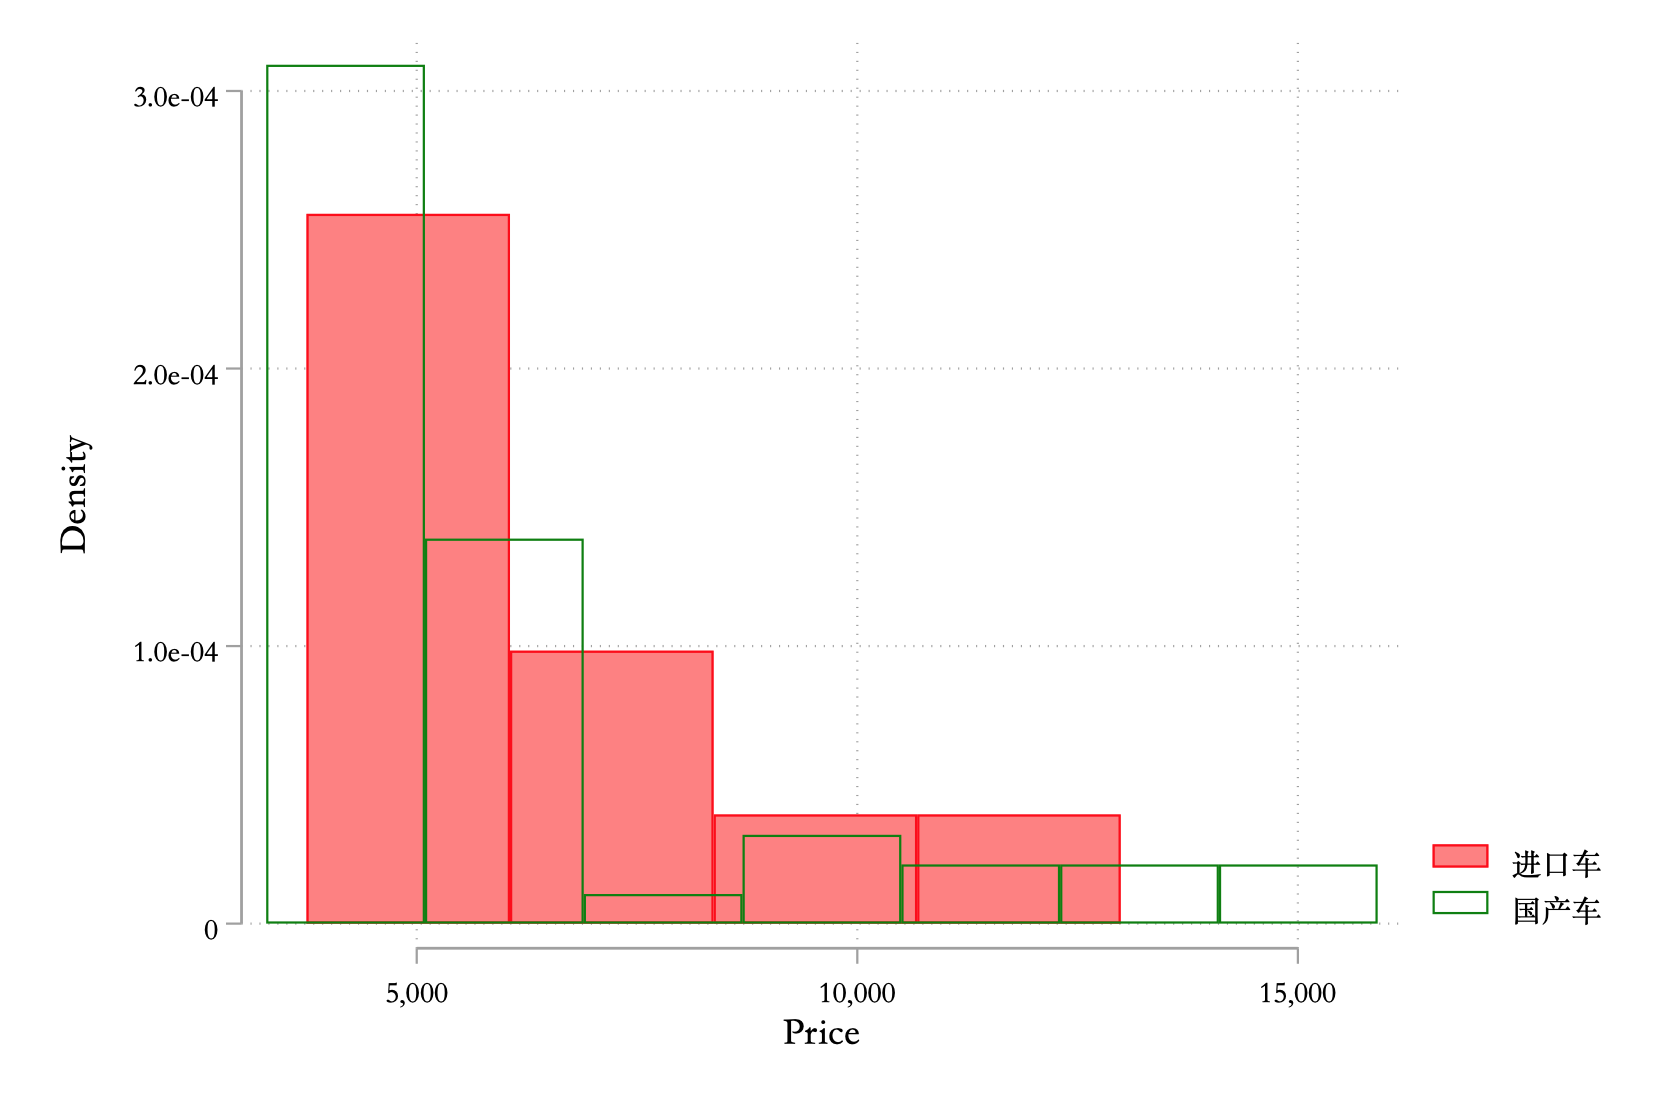
\includegraphics[width=\textwidth]{assets/histautoprice3.png}
  \caption{国产车和进口车的价格分布}\label{fig:histautoprice3}
\end{figure}

位置调整有三种,用 ggplot2 的话来说,分别是 \textcolor{third2}{identity}、\textcolor{third2}{fill} 和 \textcolor{third2}{dodge}。刚刚绘制的图 \ref{fig:stackcutclarity}就是 \textcolor{third2}{identity} 模式。除此之外,\textcolor{third2}{fill} 模式为,如图 \ref{fig:percentcutclarity}:

\begin{lstlisting}
sysuse diamonds, clear
gen id = _n
colorscheme 8, palette(Paired)
gr bar (count) id, over(clarity) over(cut) ///
    stack asyvars yti(count) ///
    leg(ti(clarity)) ///
    bar(1, color("`r(color1)'")) ///
    bar(2, color("`r(color2)'")) ///
    bar(3, color("`r(color3)'")) ///
    bar(4, color("`r(color4)'")) ///
    bar(5, color("`r(color5)'")) ///
    bar(6, color("`r(color6)'")) ///
    bar(7, color("`r(color7)'")) ///
    bar(8, color("`r(color8)'")) ///
    percent
\end{lstlisting}

\begin{figure}[htbp]
  \centering 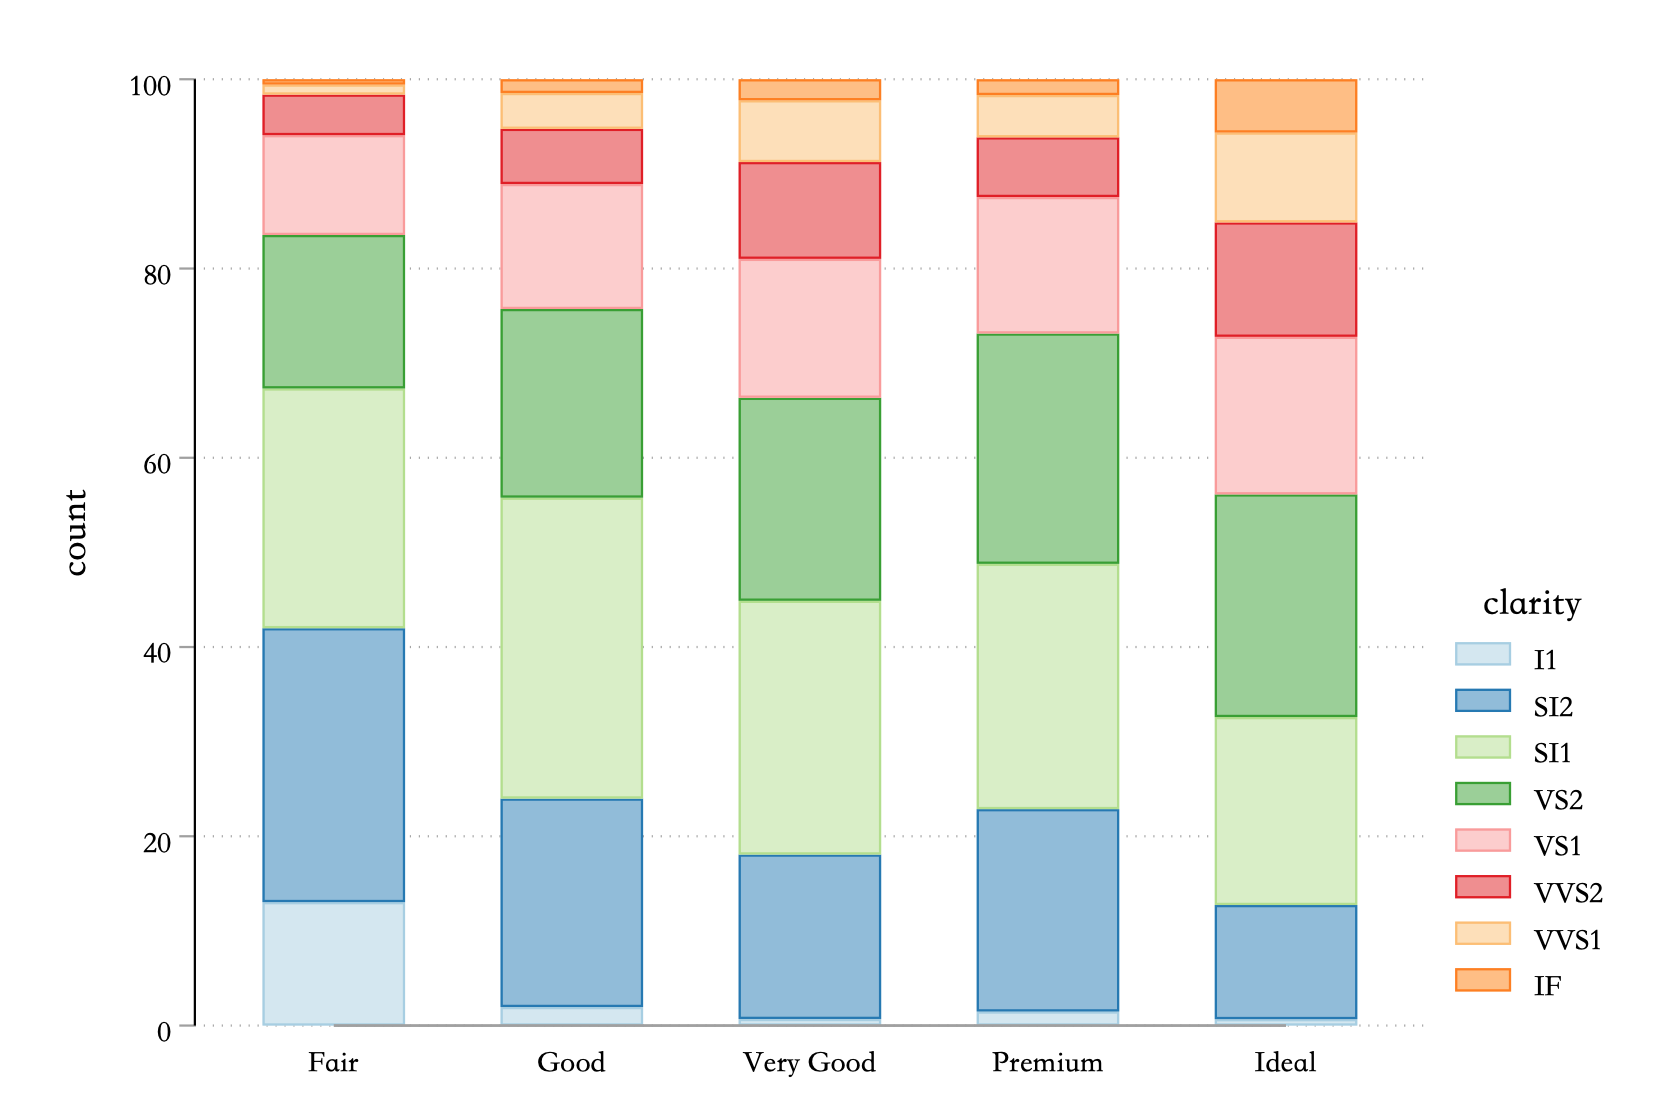
\includegraphics[width=\textwidth]{assets/percentcutclarity.png}
  \caption{钻石不同切工的克拉分布}\label{fig:percentcutclarity}
\end{figure}

最后,\textcolor{third2}{dodge} 模式为,如图 \ref{fig:dodgecutclarity}:

\begin{lstlisting}
sysuse diamonds, clear
gen id = _n
colorscheme 8, palette(Paired)
gr bar (count) id, over(clarity) over(cut) ///
    asyvars yti(count) ///
    leg(ti(clarity)) ///
    bar(1, color("`r(color1)'")) ///
    bar(2, color("`r(color2)'")) ///
    bar(3, color("`r(color3)'")) ///
    bar(4, color("`r(color4)'")) ///
    bar(5, color("`r(color5)'")) ///
    bar(6, color("`r(color6)'")) ///
    bar(7, color("`r(color7)'")) ///
    bar(8, color("`r(color8)'"))
\end{lstlisting}

\begin{figure}[htbp]
  \centering 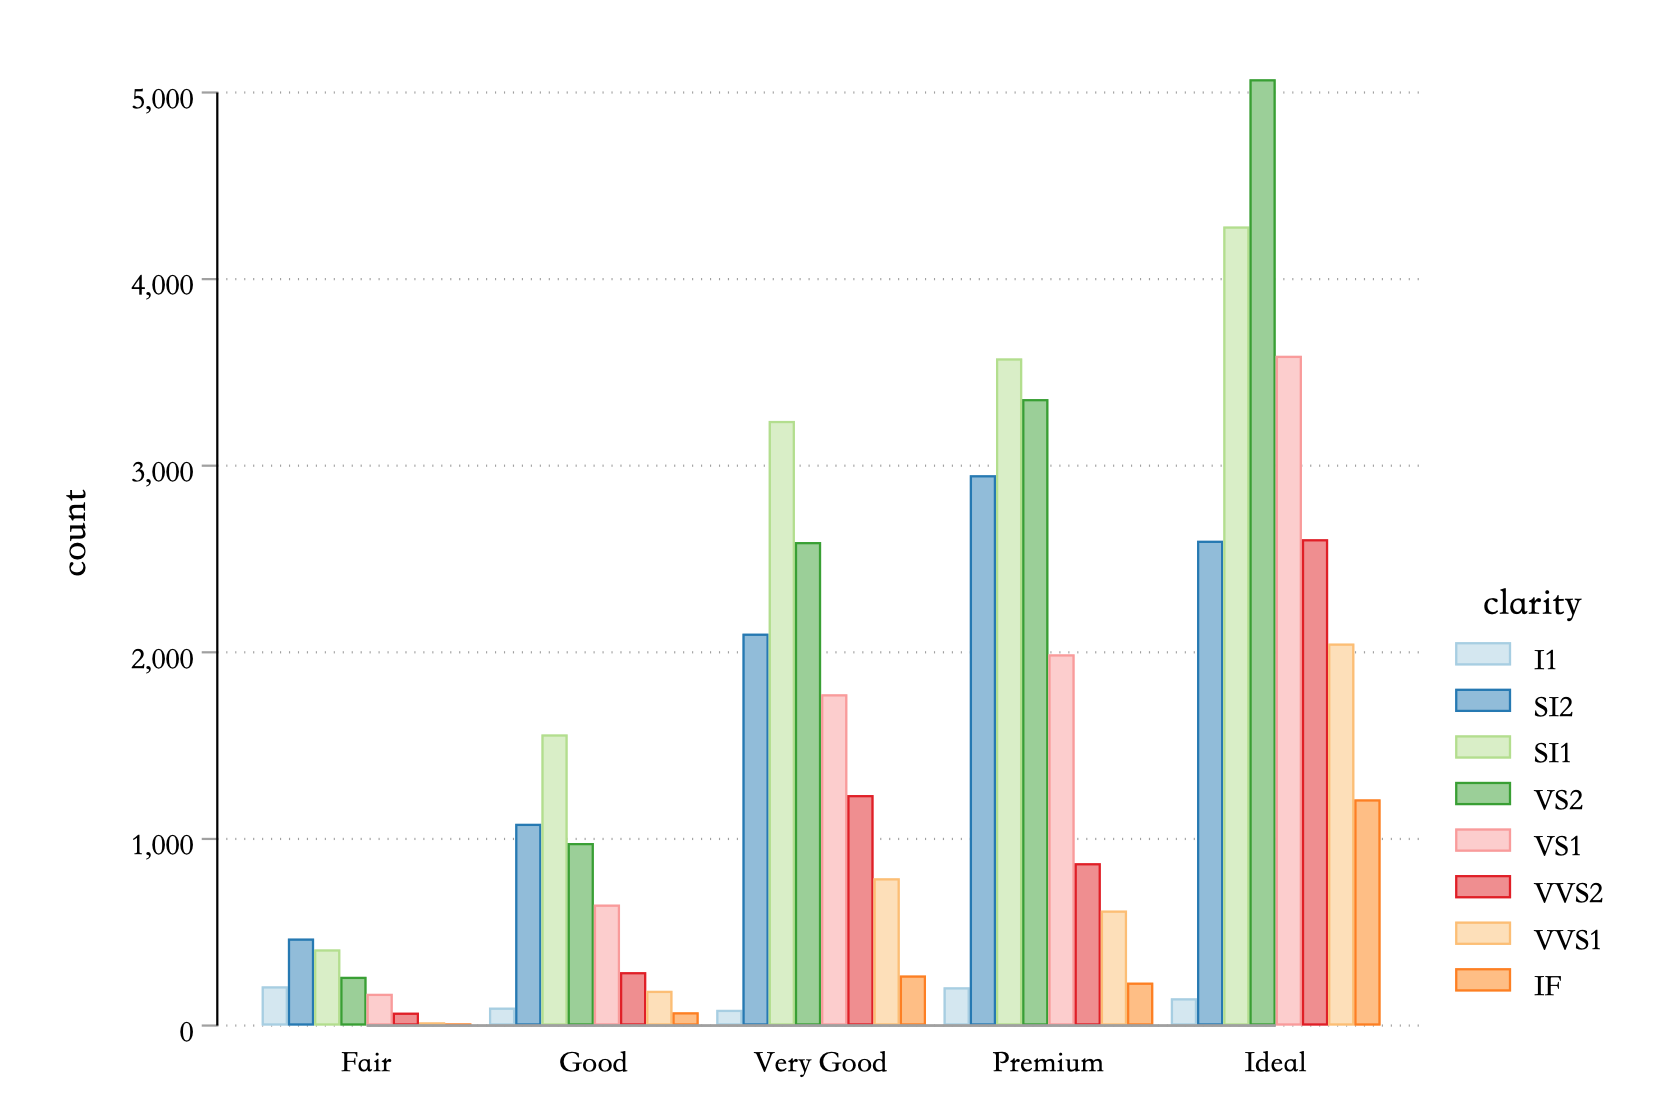
\includegraphics[width=\textwidth]{assets/dodgecutclarity.png}
  \caption{钻石不同切工的克拉分布}\label{fig:dodgecutclarity}
\end{figure}

其它类型的图其实也有位置的调整,不过不如直方图有用,例如散点图增加扰动,如图 \ref{fig:scjitter}:

\begin{lstlisting}
sysuse mpg, clear
sc hwy displ, name(p1, replace) ti(没有添加散点扰动)
sc hwy displ, name(p2, replace) jitter(3)  ti(添加了散点扰动)
gr combine p1 p2
\end{lstlisting}

\begin{figure}[htbp]
  \centering 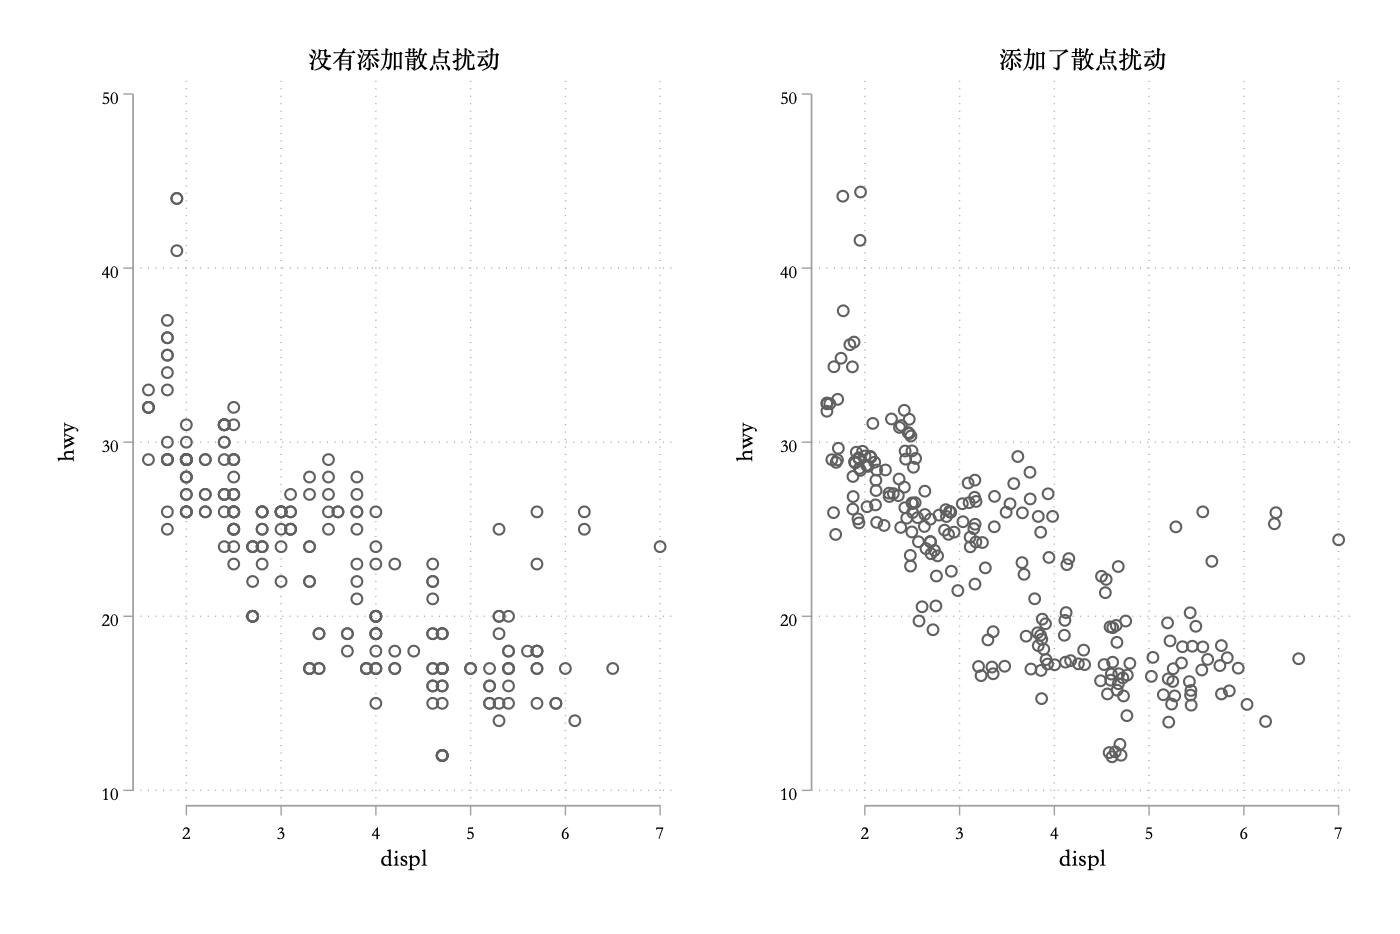
\includegraphics[width=\textwidth]{assets/scjitter.png}
  \caption{增加散点扰动的效果图}\label{fig:scjitter}
\end{figure}

很容易理解,增加散点扰动也是缓解散点重叠问题的一种办法。前面的使用透明度也是一种方法,如图 \ref{fig:scopc}。

\begin{figure}[htbp]
  \centering 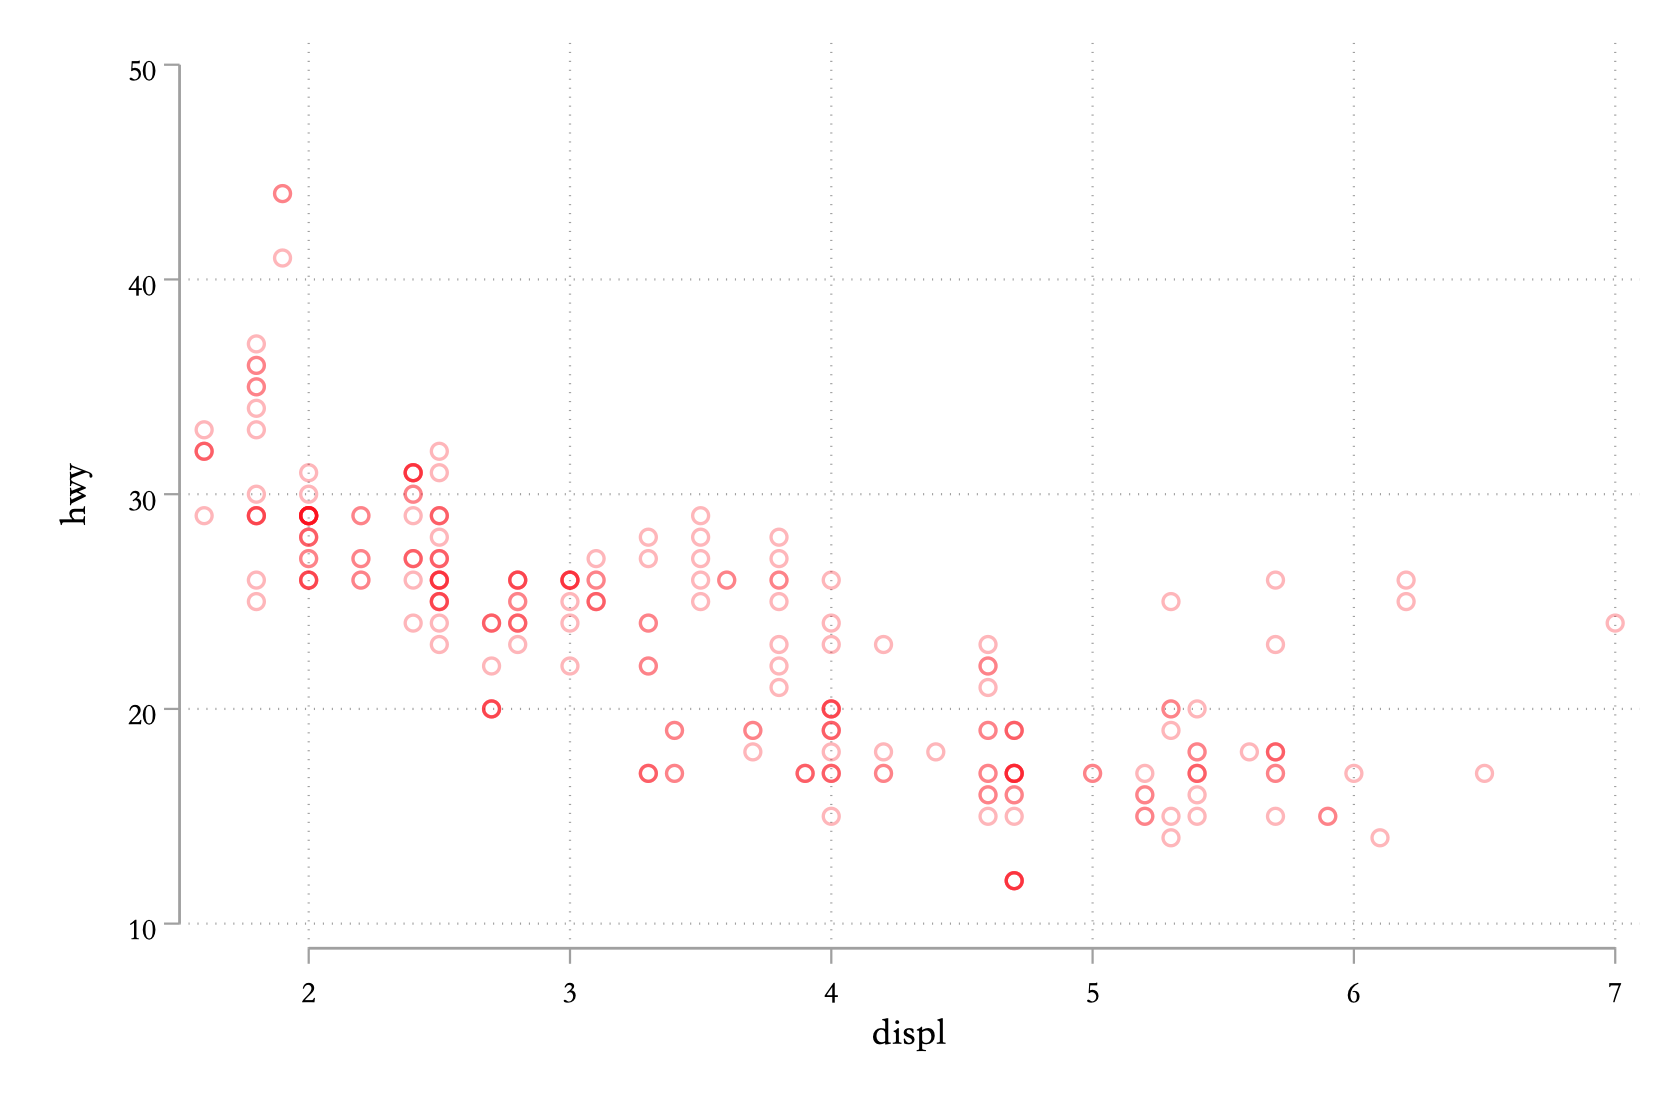
\includegraphics[width=\textwidth]{assets/scopc.png}
  \caption{使用透明度的效果图}\label{fig:scopc}
\end{figure}

这里再介绍两种减缓散点重叠问题的方法:

方法1: 使用 flower命令,如图 \ref{fig:flower}:

\begin{lstlisting}
* 安装:
ssc install flower
flower hwy displ
\end{lstlisting}

\begin{figure}[htbp]
  \centering 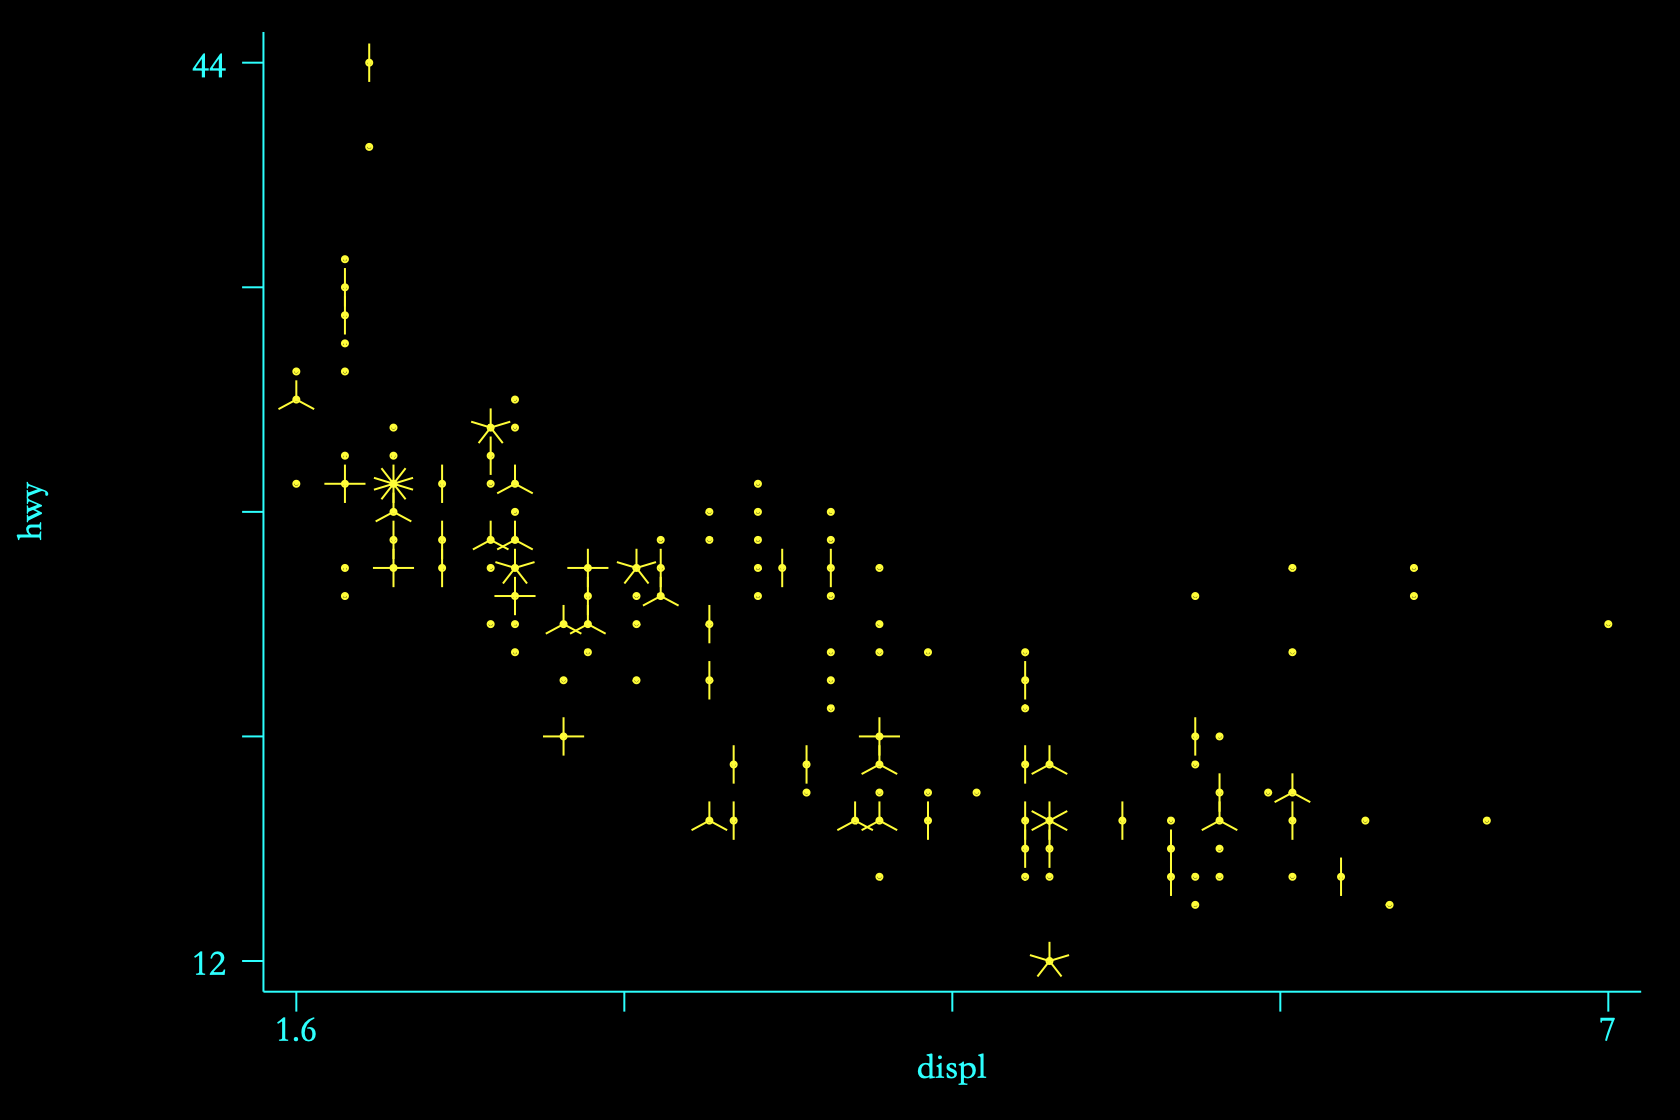
\includegraphics[width=\textwidth]{assets/flower.png}
  \caption{使用太阳花的花瓣数量表示重叠程度}\label{fig:flower}
\end{figure}

实际上,Stata官方也提供了绘制太阳花的命令,如图 \ref{fig:sunflower}:

\begin{lstlisting}
sunflower hwy displ
*> Bin width          =       .36
*> Bin height         =   2.65899
*> Bin aspect ratio   =   6.39655
*> Max obs in a bin   =        12
*> Light              =         3
*> Dark               =        13
*> X-center           =       3.3
*> Y-center           =        24
*> Petal weight       =         1
*> ------------------------------------------------------------------
*>      flower      petal     No. of     No. of  estimated     actual
*>        type     weight     petals    flowers       obs.       obs.
*> ------------------------------------------------------------------
*>        none                                          46         46
*>       light          1          3          6         18         18
*>       light          1          4          7         28         28
*>       light          1          5          8         40         40
*>       light          1          6          2         12         12
*>       light          1          7          3         21         21
*>       light          1          8          2         16         16
*>       light          1          9          1          9          9
*>       light          1         10          1         10         10
*>       light          1         11          2         22         22
*>       light          1         12          1         12         12
*> ------------------------------------------------------------------
*>                                                     234        234
\end{lstlisting}

\begin{figure}[htbp]
  \centering 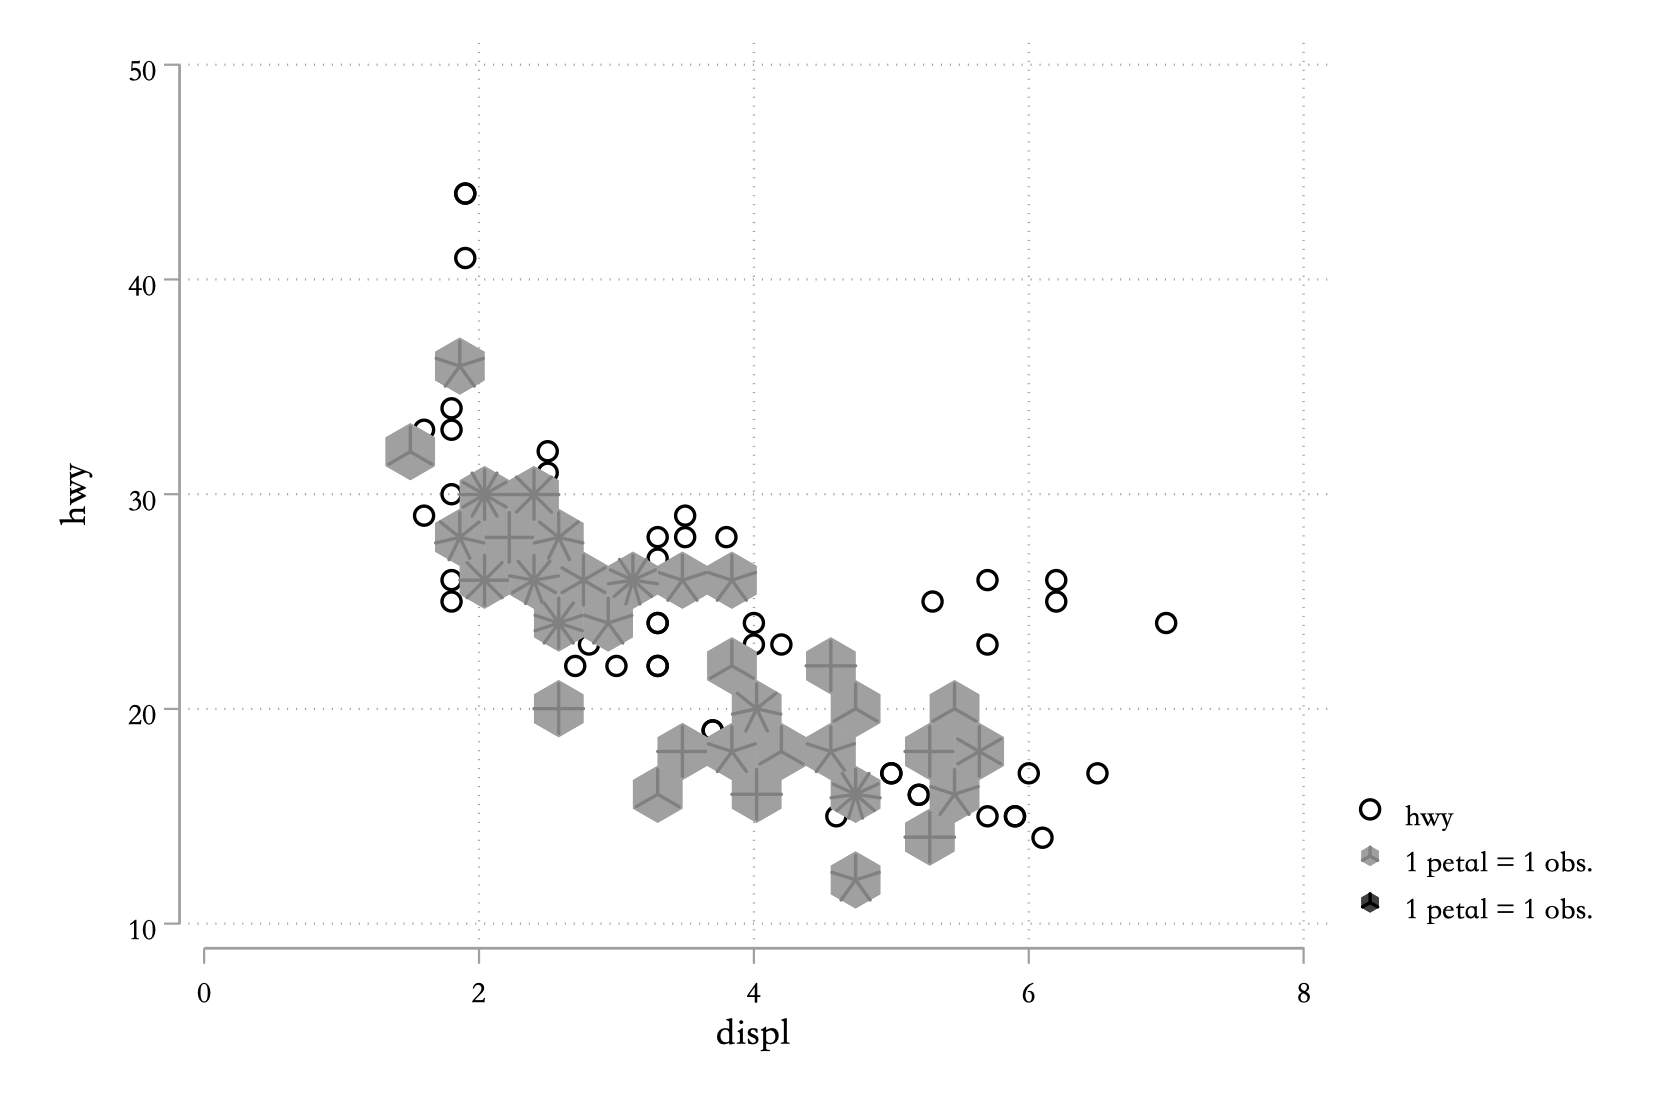
\includegraphics[width=0.8\textwidth]{assets/sunflower.png}
  \caption{使用太阳花的花瓣数量表示重叠程度}\label{fig:sunflower}
\end{figure}

另一种方法是使用 \href{https://github.com/haghish}{E. F. Haghish} 开发的 \href{https://github.com/haghish/neat}{neat} 命令,如图 \ref{fig:neatscatter}:

\begin{lstlisting}
* 安装 neat 命令
github install haghish/neat, replace
sysuse mpg, clear
neat hwy displ
sc hwy displ
\end{lstlisting}

\begin{figure}[htbp]
  \centering
  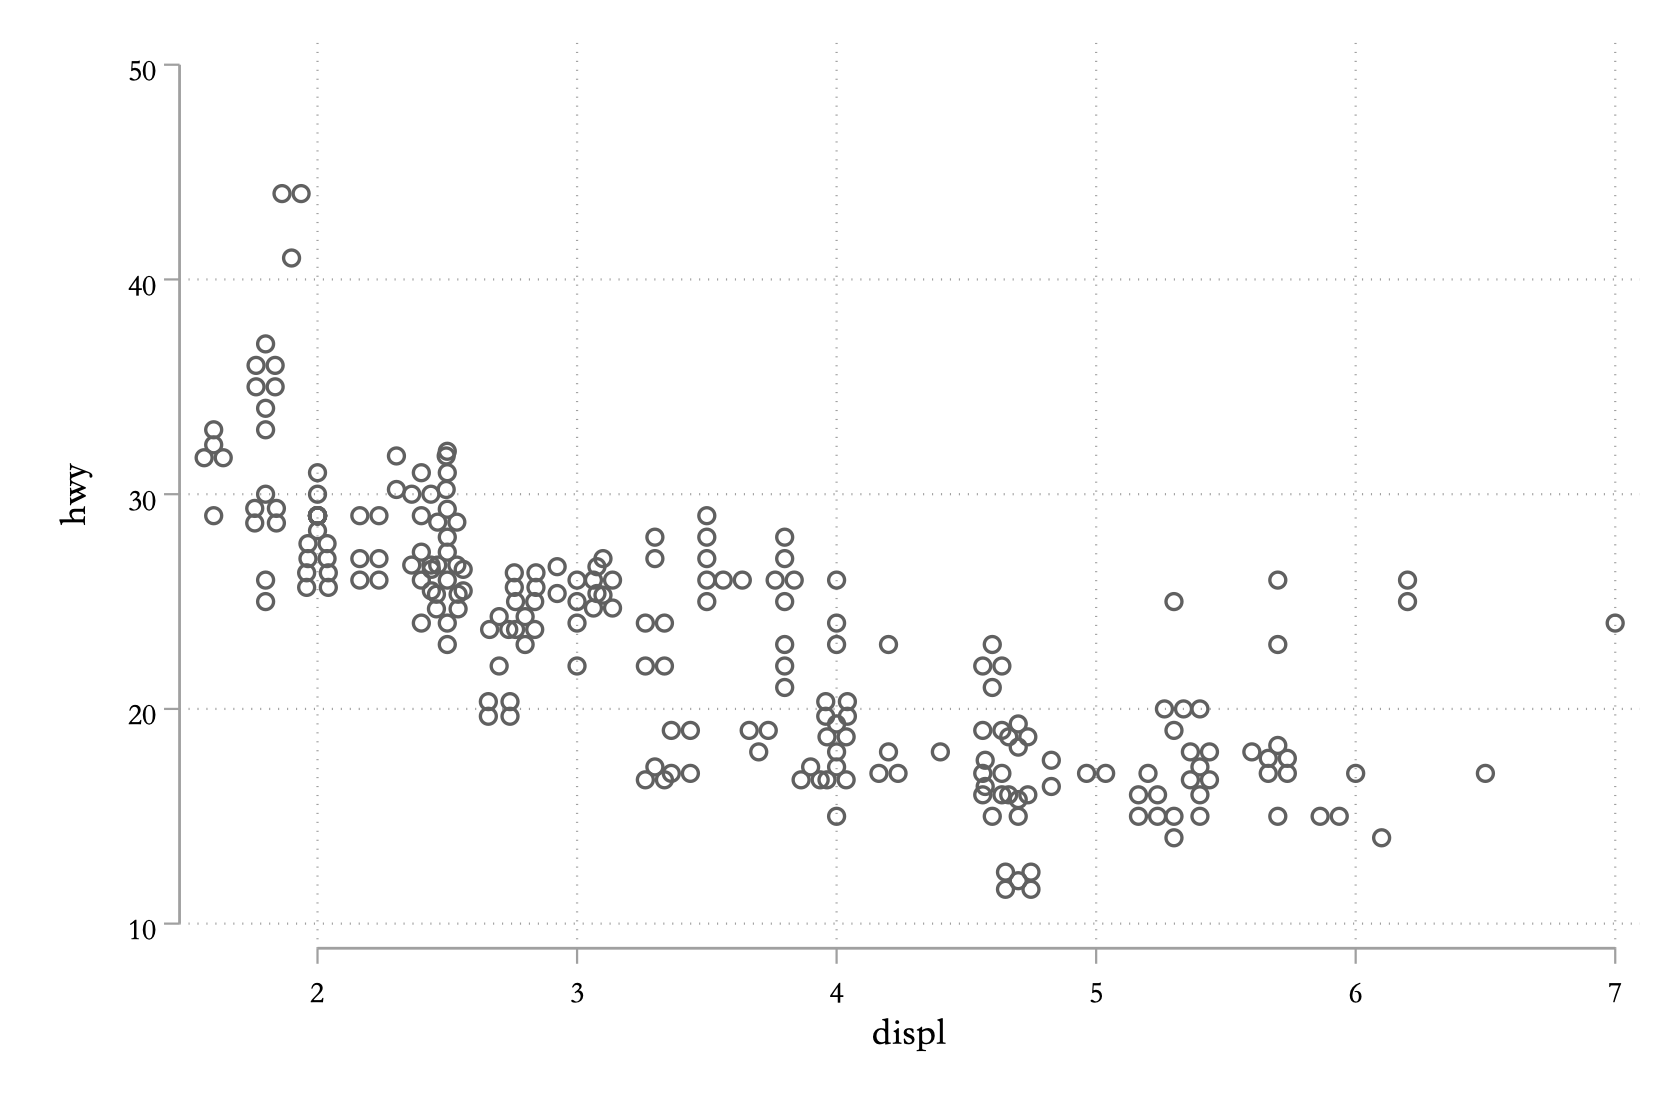
\includegraphics[width=\textwidth]{assets/neatscatter.png}
  \caption{使用太阳花的花瓣数量表示重叠程度}\label{fig:neatscatter}
\end{figure}

需要注意的是,neat并不是绘图的命令,而是一个修改数据的命令。

关于 neat 命令的详细使用介绍可以参考其 GitHub 仓库: \href{https://github.com/haghish/neat}{haghish/neat}

\section{坐标系统}

Stata 绘图中坐标系统的调整主要是横纵坐标的交换,如图 \ref{fig:boxcombine}:

\begin{lstlisting}
sysuse mpg, clear
gr box hwy, over(class) ti("绘图命令:gr box hwy, over(class)") ///
    name(p1, replace)
gr hbox hwy, over(class)  ti("绘图命令:gr hbox hwy, over(class)") ///
    name(p2, replace)
gr combine p1 p2
\end{lstlisting}

\begin{figure}[htbp]
  \centering 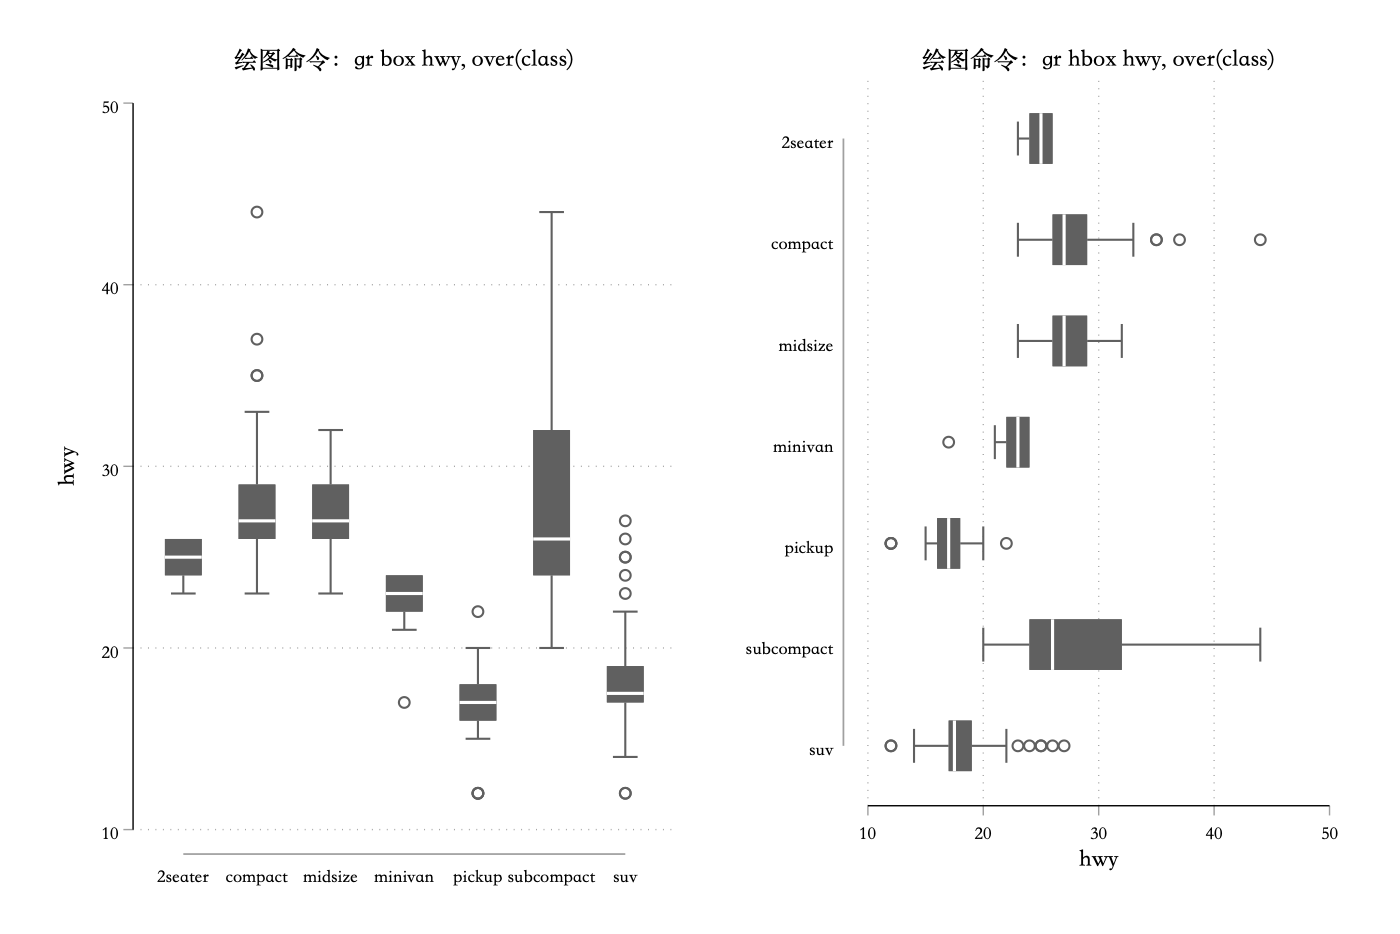
\includegraphics[width=\textwidth]{assets/boxcombine.png}
  \caption{竖直箱线图与水平箱线图}\label{fig:boxcombine}
\end{figure}

另一种常用的坐标系调整是纵轴和横轴尺度的比例,使用 \texttt{aspectratio()} 选项调整,例如我想设置纵轴和横轴的比例是 1:2,如图 \ref{fig:aspscatter}:

\begin{lstlisting}
sysuse mpg, clear
sc hwy displ, aspect(0.5)
\end{lstlisting}

\begin{figure}[htbp]
  \centering 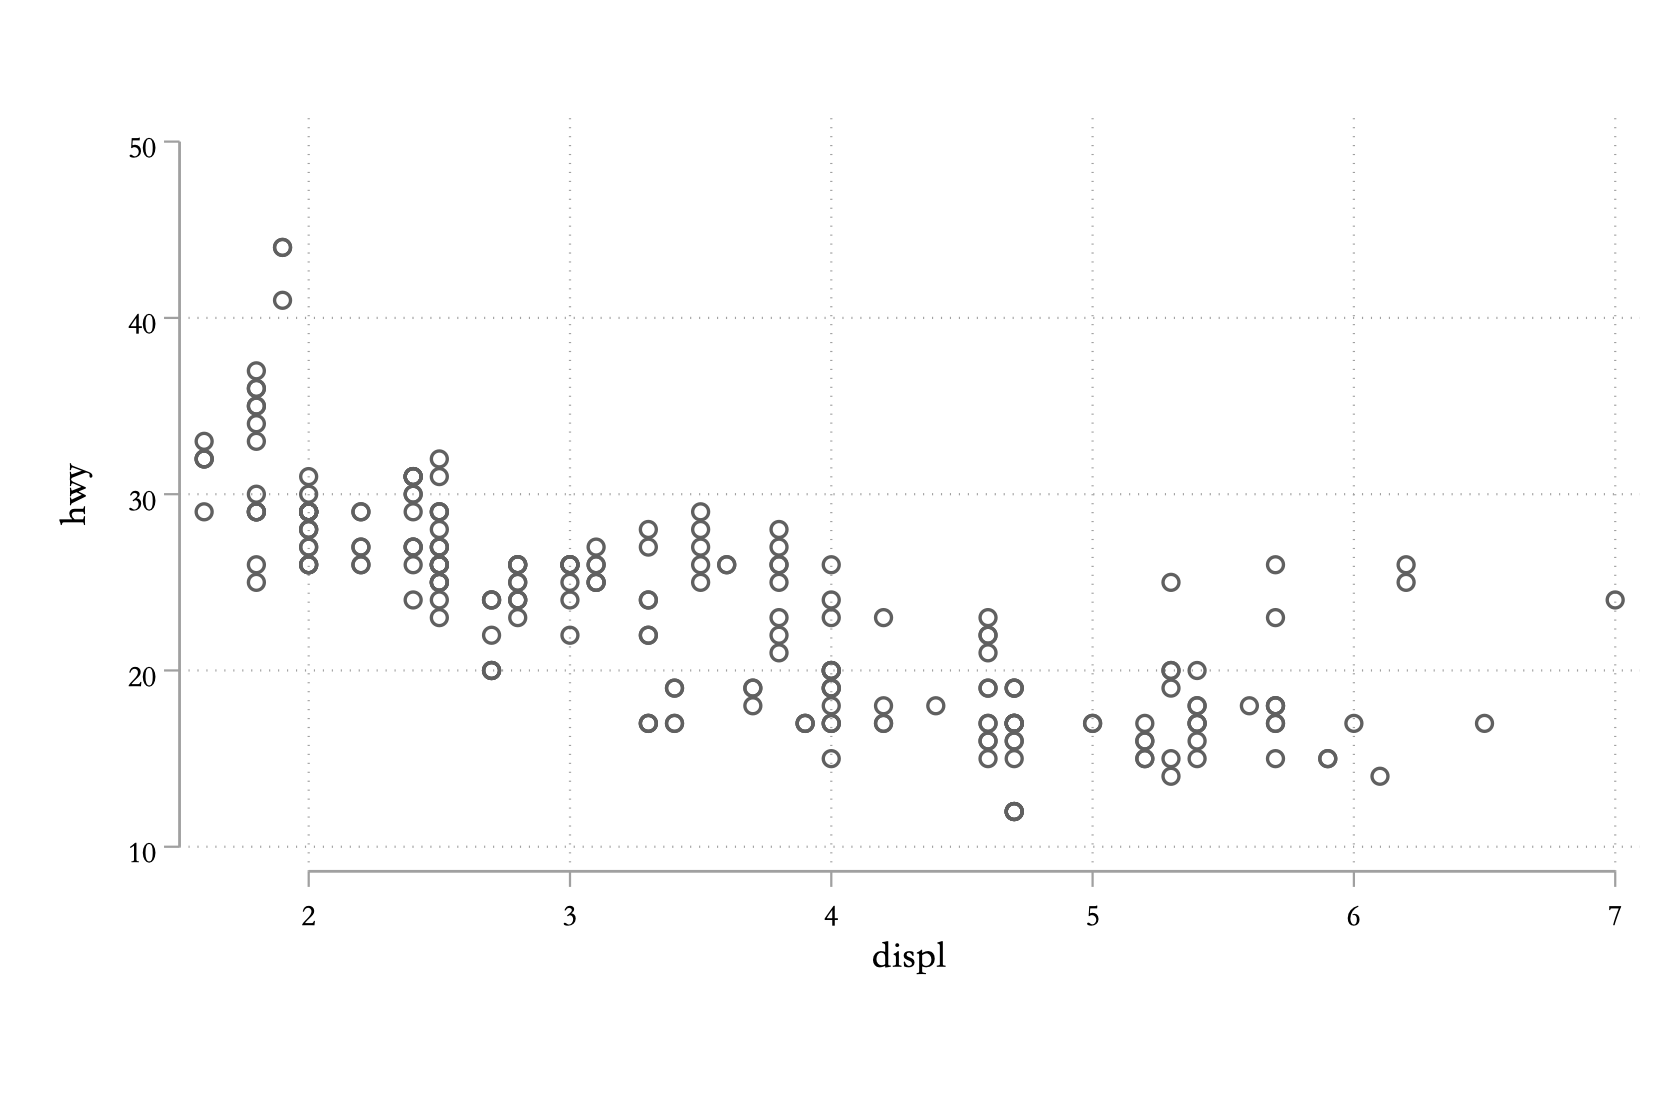
\includegraphics[width=\textwidth]{assets/aspscatter.png}
  \caption{aspectratio() 选项的使用}\label{fig:aspscatter}
\end{figure}

Stata 中并没有直接的坐标系转换机制(这就不像 ggplot2 中那么方便了),但是 Stata 中有绘制各种图的命令,以上展示的图基本都是基于笛卡尔坐标系的,基于极坐标系的饼图在 Stata 中可以直接使用 pie 命令绘制,如图 \ref{fig:barpluspie}:

\begin{lstlisting}
sysuse diamonds, clear
contract cut
colorscheme 5, palette(Paired)
tw ///
bar _freq cut if cut == 1, horizontal fc("`r(color1)'") lc("`r(color1)'") || ///
bar _freq cut if cut == 2, horizontal fc("`r(color2)'") lc("`r(color2)'") || ///
bar _freq cut if cut == 3, horizontal fc("`r(color3)'") lc("`r(color3)'") || ///
bar _freq cut if cut == 4, horizontal fc("`r(color4)'") lc("`r(color4)'") || ///
bar _freq cut if cut == 5, horizontal fc("`r(color5)'") lc("`r(color5)'") ///
    ylab(, val) name(p1, replace) nodraw leg(off)

sysuse diamonds, clear
colorscheme 5, palette(Paired)
gr pie, over(cut) ///
    pie(1, color("`r(color1)'")) ///
    pie(2, color("`r(color2)'")) ///
    pie(3, color("`r(color3)'")) ///
    pie(4, color("`r(color4)'")) ///
    pie(5, color("`r(color5)'")) ///
    name(p2, replace) leg(off) ///
    pl(1 name) ///
    pl(2 name) ///
    pl(3 name) ///
    pl(4 name) ///
    pl(5 name) nodraw
gr combine p1 p2
\end{lstlisting}

\begin{figure}[htbp]
  \centering 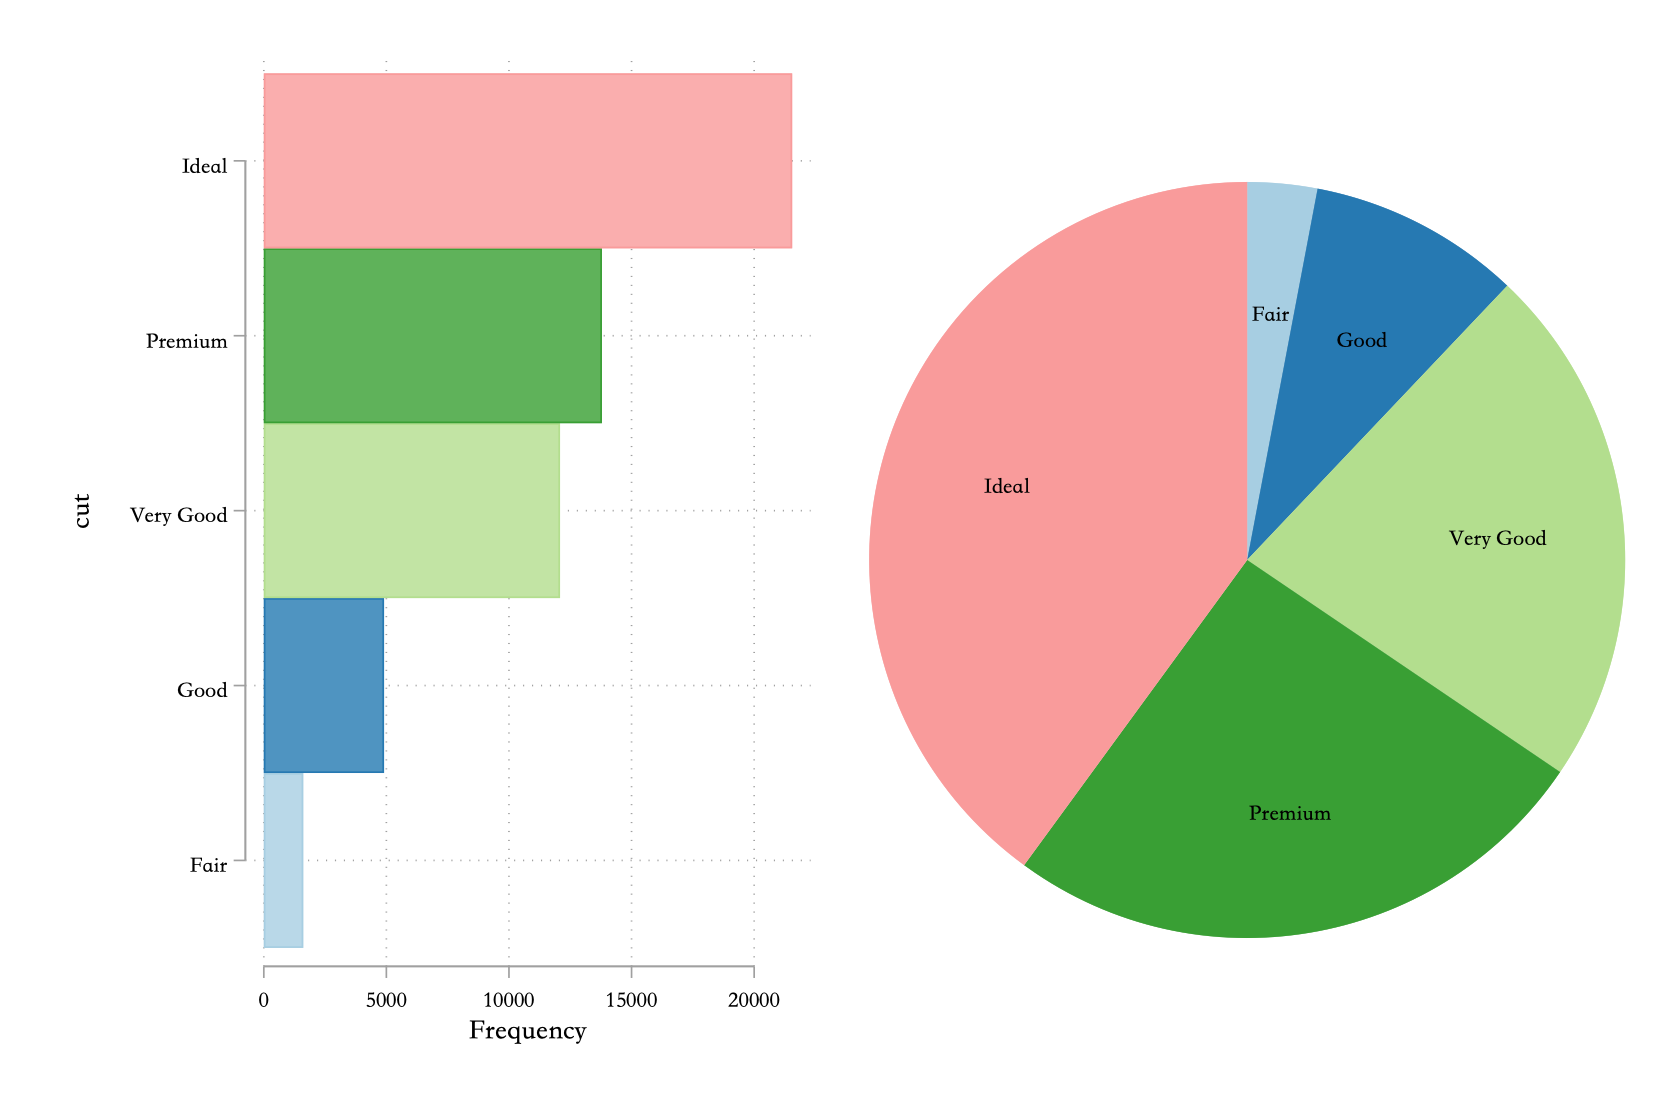
\includegraphics[width=\textwidth]{assets/barpluspie.png}
  \caption{graph bar 和 graph pie 命令的使用}\label{fig:barpluspie}
\end{figure}

这里我们使用了一个新的选项 \texttt{horizontal},这个选项控制图像的水平显示。

最后我们再回到 \texttt{aspectratio()} 选项上,经常我们需要在图像中添加一条45线,例如绘制 QQ 图的时候就需要添加一条45度线,这个时候使用 \texttt{aspect(1)} 可以保证这条45度线是真的45度线,如图 \ref{fig:qnorm}:

\begin{lstlisting}
qnorm depth, aspect(1) xlab(40(10)80) ylab(40(10)80)
\end{lstlisting}

\begin{figure}[htbp]
  \centering 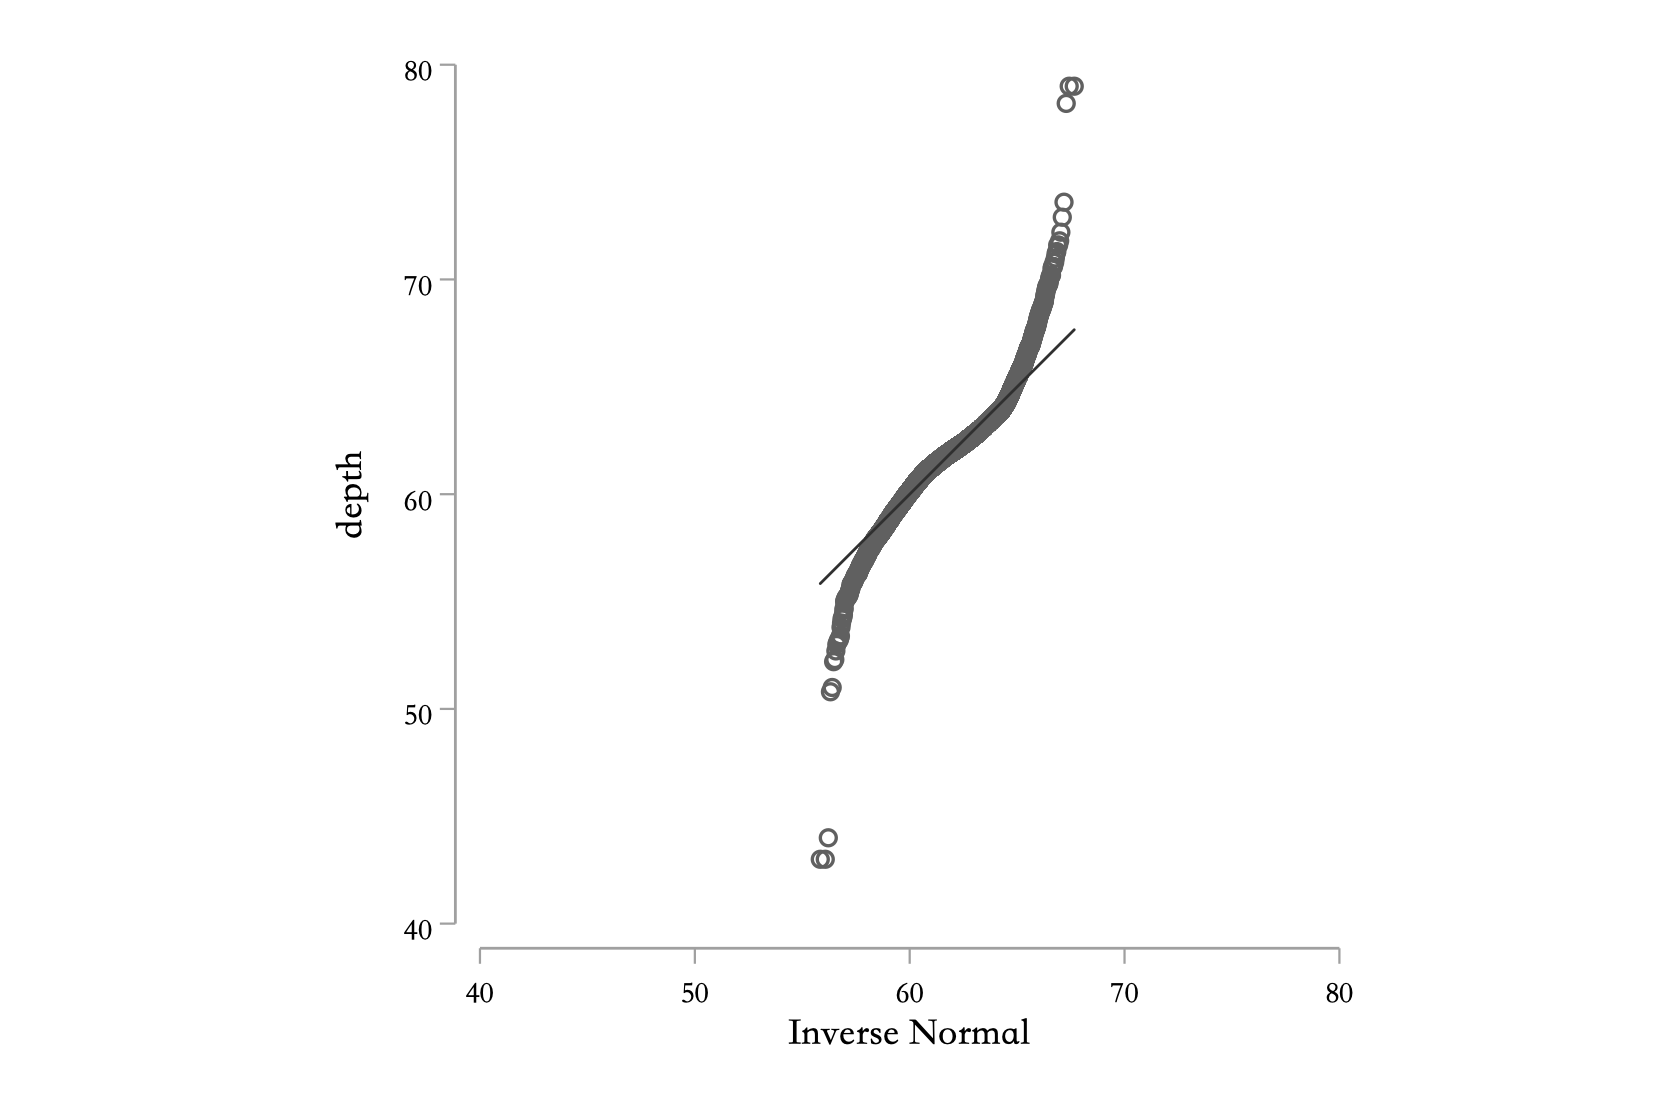
\includegraphics[width=\textwidth]{assets/qnorm.png}
  \caption{depth 变量的 QQ 图}\label{fig:qnorm}
\end{figure}
